\documentclass[a4paper, 12pt]{article} %\documentclass[]{article}
\usepackage[utf8]{inputenc}

\usepackage{setspace}
\onehalfspace

\usepackage{graphicx}
\usepackage{float} % H positioning
\usepackage{lscape}

\usepackage{listings}

\usepackage [english]{babel}
\usepackage [autostyle, english = american]{csquotes}

\usepackage[caption = false]{subfig}

% head and footer
\usepackage{fancyhdr}
\pagestyle{fancy}
\fancyhf{}
\fancyhead[LE,RO]{\thepage}
\fancyhead[RE,LO]{\leftmark}
%\fancyfoot[CE,CO]{\leftmark}
%\fancyfoot[LE,RO]{\thepage}
\fancyfoot[LE,RO]{\thepage}
\fancyfoot[RE,LO]{\rightmark}
\renewcommand{\headrulewidth}{2pt}
\renewcommand{\footrulewidth}{1pt}


%code
\usepackage{lmodern}  % for bold teletype font
\usepackage{amsmath}  % for \hookrightarrow
\usepackage{amssymb} % for math symbols
\usepackage{xcolor}   % for \textcolor
\usepackage{tabularx}

\usepackage{booktabs} % for tables https://people.inf.ethz.ch/markusp/teaching/guides/guide-tables.pdf
\newcommand{\ra}[1]{\renewcommand{\arraystretch}{#1}}

\usepackage{multirow}


\definecolor{eclipseStrings}{RGB}{42,0.0,255}
\definecolor{eclipseKeywords}{RGB}{127,0,85}
\colorlet{numb}{magenta!60!black}
\lstdefinelanguage{json}{
	basicstyle=\normalfont\ttfamily,
	commentstyle=\color{eclipseStrings}, % style of comment
	stringstyle=\color{eclipseKeywords}, % style of strings
	numbers=left,
	numberstyle=\scriptsize,
	stepnumber=1,
	numbersep=8pt,
	showstringspaces=false,
	breaklines=true,
	frame=lines
	string=[s]{"}{"},
	comment=[l]{:\ "},
	morecomment=[l]{:"},
	literate=
	*{0}{{{\color{numb}0}}}{1}
	{1}{{{\color{numb}1}}}{1}
	{2}{{{\color{numb}2}}}{1}
	{3}{{{\color{numb}3}}}{1}
	{4}{{{\color{numb}4}}}{1}
	{5}{{{\color{numb}5}}}{1}
	{6}{{{\color{numb}6}}}{1}
	{7}{{{\color{numb}7}}}{1}
	{8}{{{\color{numb}8}}}{1}
	{9}{{{\color{numb}9}}}{1}
}

\usepackage[hidelinks]{hyperref}


\begin{document}
	
	%opening
	\begin{titlepage}
		\centering
		\vspace*{1cm}
		%\includegraphics[width=0.20\textwidth]{images/logo_unipd.png}\par\vspace{1cm}
		{\par \scshape\LARGE Università degli Studi di Padova \par}
		\vspace{1cm}
		{\scshape\Large Department of Information Engineering\\Master Thesis in Computer Engineering\par}
		\vspace{1.5cm}
		{\huge\bfseries Online Contextual System Tuning with Bayesian Optimization and Workload Forecasting\par}
		\vspace{2cm}
		{ \large \itshape Master Candidate:}
		{ \large Luca \textsc{Moroldo} \par}
		\vspace{0.7cm}
		{ \large \itshape Supervisor:}
		{ \large Prof. Nicola \textsc{Ferro} \par}
		\vfill
		
		% Bottom of the page
		{ \large XX February 2022 \par}
		{ \large \textsc{Academic Year 2021/2022}\par}
	\end{titlepage}
	
	% empty page
	\clearpage%
	\thispagestyle{empty}%
	\addtocounter{page}{-1}%
	\null%
	\clearpage
	
	\newpage
	\pagenumbering{roman}
	\thispagestyle{plain}
	\section*{Summary}
	This thesis presents the work done to extend an existing software systems tuner to be applied on a production environment according to the real workload perceived by the system, i.e. while it is serving its clients.
	To do so, two main modules were developed: a forecasting module, based on state-of-the-art techniques that minimize the necessity of manual work, and a stability finder module, used to decide when to perform tuning experiments. With these two modules, the probability of testing a new software configuration during a workload change is reduced, which would cause the system clients to suffer Quality of Service losses.
	Moreover, by directly tuning the production system the effort of applying the tuner is reduced so that it can be easily and quickly applied to different scenarios.
	The proposed solution was tested on two DBMS models with 20 scenarios, highlighting that the integration of forecasting techniques improves the safety of the tuning process while keeping the effectiveness of the original tuner.
	
	% empty page
	\clearpage%
	\thispagestyle{empty}%
	\addtocounter{page}{-1}%
	\null%
	\clearpage
	
	% Custom TOC title
	\renewcommand{\contentsname}{Index}
	\newpage
	\thispagestyle{plain}
	\tableofcontents

	% empty page
	\clearpage%
	\thispagestyle{empty}%
	\addtocounter{page}{-1}%
	\null%
	\clearpage
	
	
	% =================== INTRODUZIONE ==========================
	
	\newpage
	\pagenumbering{arabic}
	
	\section{Introduction }
	% should i specify that the workload is also specific to each tuning scenario?
	Most software systems allow their users to tailor the configuration according to the context under which the system is running so that it can meet some quality or cost targets. With the number of available options increasing over time, the configuration spaces became too wide and the effects of their options may not be trivial or predictable, especially when many of them are tuned together. Within this context, manually finding the configuration that maximizes the performance of a web application or minimizes the costs of a cloud service requires a lot of work that can only be done by experts that know the software being tuned, consuming time and without any guarantee that such configuration will be found. Furthermore, if such optimal configuration is found, a software change or update, or even a hardware change may require the whole work to be repeated.
	
	To solve this issue, automated approaches have emerged \cite{AkamasCGP, LearningToSample, OtterTune, OtterTune2}, with Bayesian Optimization playing an important role in the field. In many cases, the available approaches explore the configuration space to build a performance model by running experiments on a replica of the real system. Performing such experiments can be expensive: replicating the entire production system may need a significant amount of resources, and most of all require understanding and analyzing the workload requested by the system's clients so that it can be replayed on the replica. The workload not only changes over time both in terms of demand and type of requests, but it can also evolve with the capabilities of the system or the acquisition of new clients (e.g. if the system is released to a new country). Any of these changes would require the analysis of the workload to be repeated so that the tuning experiments can be as likely as possible.
	
	This work builds on \cite{AkamasCGP} to directly tune the production system, avoiding the workload analysis and replication steps. Such an approach opens a new challenge: the exploration of the configuration space on the production system is vulnerable to ``bad'' configurations that can lead to low Quality of Service levels or even system failures.  We tackle this challenge with a proactive and automatic approach that makes use of workload forecasting to run tuning experiments only when the workload is predicted to be stable and suggest a workload-tailored configuration, minimizing the probability of failure and opening the possibility of preemptively applying the best configuration found for the upcoming workload. 
	
	We further present the problem in section \ref{sec:context_and_state_of_the_art}, detailing the components required by the approach and the current state of the art. Section \ref{sec:proposed_solution} describes the proposed solution and \ref{sec:exp_setup} the experimental setup. Finally, section \ref{sec:results} shows the results obtained on two distinct database models.
	
	\section{Context and State of the Art } \label{sec:context_and_state_of_the_art}
	Tuning an IT system without changing its code requires finding good configurations in an enormous search space where the tunable parameters affect different layers of the IT stack, such as Operating System (OS), Database Management System (DBMS), and Java Virtual Machine (JVM). These parameters can have counter-intuitive effects with inter-dependencies, making manual optimization hard or even unfeasible when looking for the optimal configuration. Recent years have seen automatic approaches emerge \cite{AkamasCGP, OtterTune, OtterTune2, LearningToSample}, with \cite{AkamasCGP} using Contextual Bayesian Optimization (BO). However, when automatically tuning IT systems on a staging environment, i.e. a replica of the real system, it is still necessary to replicate the real workload to find the optimal configuration that fits the way the IT system is used at different times of the day or week. Finding such workload(s) takes time, lengthening the time required to complete the tuning process.
	
	A possible solution to this issue is to directly tune the production system under the real workload, removing the workload analysis and replication requirement, with the performance of each configuration measured directly from the production system rather than a staging replica, which could lead to unrealistic outcomes. However, performing experiments on an IT system while being used can be dangerous and pose new challenges: a bad configuration can cause a bad user experience and consequently business issues.
	
	This work extends the Contextual Bayesian Optimization tuner \cite{AkamasCGP} to be applied in an online manner	on IT systems receiving the production workload by providing two key components: a workload characterization and a workload forecasting module. \\
	The following section briefly presents BO and section \ref{ssec:contextual_bayesian_optimization} presents the Contextual BO tuner of \cite{AkamasCGP} explaining why workload characterization and forecasting are required. The state of the art of forecasting is presented (section \ref{sec:forecasting}), followed by a section on workload forecasting in the context of IT systems (section \ref{ssec:workload_forecasting}). A general overview of workload characterization is presented in section \ref{ssec:workload_characterization}. Clustering, which can be used for workload characterization, is described in section \ref{ssec:clustering}.
	
	\subsection{Bayesian Optimization } \label{ssec:bayesian_optimization}
	Bayesian Optimization \cite{BO} is a tool for the joint optimization of design choices of complex systems, such as the parameters of a recommendation system, a neural network, or a medical analysis tool. For example a typical software system made of a database, a back-end, and a front-end is characterized by an enormous amount of parameters that are often dependent on each other.
	Optimizing such parameters is not a simple task, and BO provides an automated approach to make such design choices.\\
	
	Mathematically, the goal is to maximize (or minimize) an unknown objective function $f$:\\
	\begin{equation} \label{eq:bo_optimization}
				\pmb{x}^\star = \underset{\pmb{x} \in \mathcal{X}}{\mathrm{argmax}} f(\pmb{x})
	\end{equation}
	where $\mathcal{X}$ is the design space of interest, e.g. a compact subset of $\mathbb{R}^d$. In general, $f$ can be any black-box function with no simple closed form that can be evaluated at any arbitrary point in the domain $\mathcal{X}$, where the evaluation can produce noise-corrupted outputs $y \in \mathbb{R}$.\\
	BO is a sequential approach to solve equation \ref{eq:bo_optimization}: at every iteration $i$, the algorithm selects a new $\pmb{x}_{i+1}$ at which $f$ is queried, resulting in a measurement $y_i$. When the maximum number of iterations is reached, or when $y^\star$ is a satisfactory outcome, the algorithm stops returning the best configuration $\pmb{x}^\star$ associated with the best outcome $y^\star$. BO is very data efficient, making it useful when the evaluations of $f$ are costly: the model is initialized with a prior belief, and then at each iteration it is refined using observed data via Bayesian posterior updating. The acquisition function $\alpha_n : \mathcal{X} \rightarrow \mathbb{R}$ guides exploration by evaluating candidate points in $\mathcal{X}$, meaning that $\pmb{x}_{i+1}$ is selected by maximizing $\alpha_n$ using data up to iteration $i$. Figure \ref{fig:bo} shows a few iterations of BO.
	\begin{figure} \label{fig:bo}
		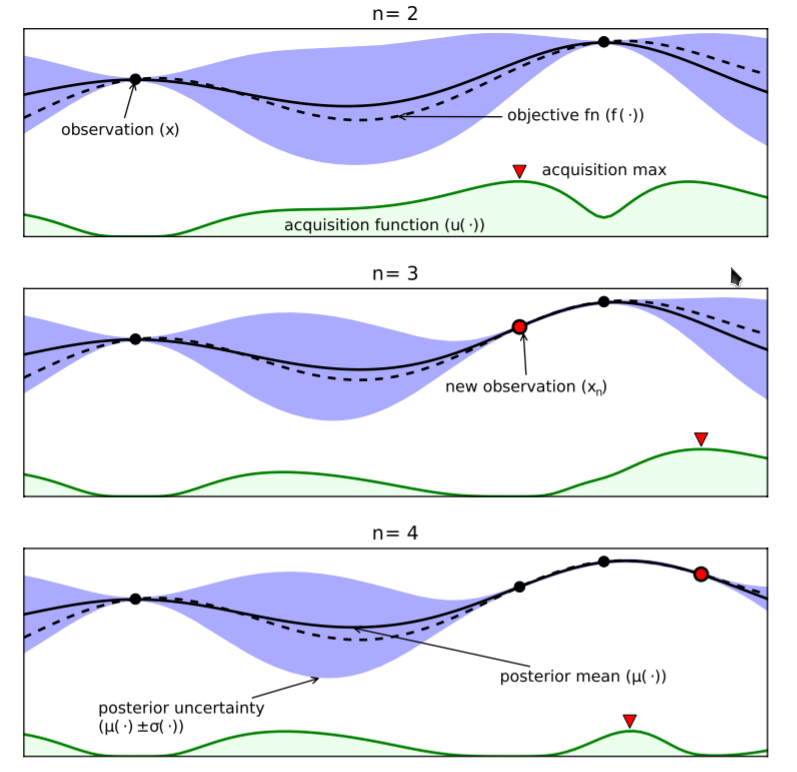
\includegraphics[width=\linewidth]{img/bo.png}
		\caption{A few iterations of BO. The acquisition function in green guides the selection of the next point, obtaining a new observation $(\pmb{x}_i, y_i)$} that updates the underlying model.
	\end{figure}
	The acquisition function $\alpha_n$ provides a trade off between exploration and exploitation: when boosting exploration the value of $\alpha_n$ will be higher in areas of uncertainty, while when boosting exploitation $\alpha_n$ will favor locations where the surrogate model predicts a high objective. It is critical for the acquisition function to be cheap to evaluate or approximate, especially in relation to the objective function $f$.
	
	In summary, BO has two key ingredients \cite{BO}: a probabilistic surrogate model, consisting of a prior distribution that captures our beliefs about $f$ and an observation model that describes the data generation process, and a loss function that describes how optimal a sequence of queries are. The expected loss is minimized to drive the selection of $\pmb{x}_i$. After observing the outcome $y_i$ of $\pmb{x}_i$, the prior is updated to produce a more informative posterior distribution.
	
	Finally, when dealing with a family of correlated objective functions $\mathcal{T}=\{f_1, ..., f_m\}$, such as the performance of an IT system under different workloads or the same IT system running with different software versions, it may be useful to use data obtained optimizing $\{f_1, ..., f_{j-1}, f_{j+1}, ..., f_m\}$ to optimize $f_j$. BO has been extended to deal with such multitask scenario \cite{CGPBanditOptimization} by sharing information between the black-box functions in $\mathcal{T}$: figure \ref{fig:multitask_bo} shows how data from two functions influence the posterior predictive distribution of another function.
	\begin{figure} \label{fig:multitask_bo}
		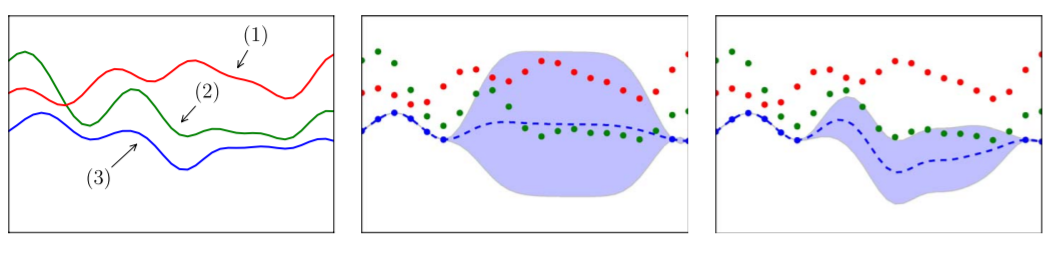
\includegraphics[width=\linewidth]{img/multitask_bo.png}
		\caption{Multitask Bayesian Optimization. The figure in the middle shows the posterior predictive distribution of the blue function (3) without exploiting the information of the other functions.}
	\end{figure}
	
	\subsubsection{Contextual Bayesian Optimization of IT systems} \label{ssec:contextual_bayesian_optimization}
	
	When applying BO to IT systems, the goal is to find a configuration $\pmb{x}$ to optimize a performance indicator $y \in \mathbb{R}$ such as throughput, response time, and memory consumption \cite{AkamasCGP}. If BO is applied while the system is running, it is very likely that the workload will change over time: the number of users connected to the system can increase and decrease, as their behavior can change from read-intensive to write-intensive operations. Such changes will inevitably affect how the system behaves under a specific configuration, but regardless the workload, the underlying system maintains some of its properties. This scenario perfectly fits the multitask extension of BO \cite{CGPBanditOptimization}.
	
	More formally, we are trying to maximize a function $f_{\pmb{w}}$ subject to a workload $\pmb{w}_t$ that changes over time. The tuning process, shown in figure \ref{fig:cgp_it_sys}, starts with a configuration $\pmb{x}_0$ (usually the default configuration, called baseline or vendor configuration) applied under a workload $\pmb{w}_0$ whose performance indicator $y_0$ is measured. The tuner uses a knowledge base, initially containing only the triplet $\{(\pmb{x}_0, \pmb{w}_0, y_0)\}$, along with the current workload $w_1$ to suggest a new configuration $x_1$ that is applied, evaluated, and added to the knowledge base. After $N$ iterations the tuner can exploit all information $(\{(\pmb{x}_0, \pmb{w}_0, y_0)\}, ..., \{(\pmb{x}_N, \pmb{w}_N, y_N)\})$ gathered so far to make refined suggestions.
	\begin{figure} \label{fig:cgp_it_sys}
		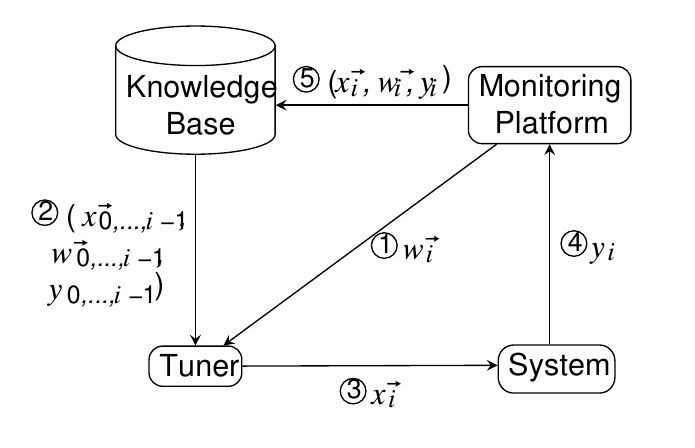
\includegraphics[width=\linewidth]{img/cgp_it_sys.png}
		\caption{BO-based tuning process. Given the workload $\pmb{w}_i$, the tuner uses the knowledge base to apply a new configuration $\pmb{x}_i$ that is evaluated (obtaining $y_i$), growing the knowledge base.}
	\end{figure}
	
	Furthermore, when optimizing a system, it may be useful to define some constraints the system should not violate: a tuning process may be executed with the requirement of satisfying some Quality of Service (QoS) levels. For example, while trying to minimize the average memory usage to reduce the infrastructure costs, the system could be expected to keep the users' requests latency below some target.  \\
	The work proposed by \cite{AkamasCGP} has been extended so that it is possible to define such constraints: when a configuration violates any constraint, the violation is added to the knowledge base along along with its configuration and associated system performance. Interestingly, by penalizing violations, the tuner can be used on a system that doesn't initially satisfy some QoS levels, so that at the end of the tuning process violations are not likely to occur anymore.
	
	The BO regression model of \cite{AkamasCGP} is a Gaussian Process (GP) which derives its posterior model (i.e. the predictions) by combining observed values with its prior distribution. To make GP able to explore uncertain regions, i.e. configurations that are different from the ones in the knowledge base, it should not resort to its prior distribution \cite{AkamasCGP} so that unknown configurations are not predicted to downgrade the performance of the IT system. To do so, the observed data is standardized and GP will predict that by picking a random configuration the system will exhibit a performance value that is equal to the average performance of the observed values. Nonetheless, when dealing with different workloads, it is crucial to standardize each point by taking into account the relevant workload \cite{AkamasCGP}. This can be achieved by using a modified version of the Normalized Performance Improvement:\\\\
	\centerline{
	$
	NPI(\pmb{x}, \pmb{w}) = \frac{f(\pmb{x}_0, \pmb{w}) - f(\pmb{x}, \pmb{w})}{f(\pmb{x}_0, \pmb{w}) - f(\pmb{x}^+_{\pmb{w}}, \pmb{w})}
	$
	}\\\\
	where $\pmb{x}$ is the configuration being evaluated, $\pmb{x}_0$ is the baseline configuration, $\pmb{w}$ is the workload, and $f(\pmb{x}^+_{\pmb{w}}, \pmb{w})$ is the best configuration found so far while tuning the system with the workload $\pmb{w}$. Hence, \cite{AkamasCGP} requires a workload characterization module (discussed in section \ref{ssec:workload_characterization}) to cluster the workloads and effectively apply BO.
	
	To evaluate the performance of an IT system under a new configuration, many technologies require some warm-up time. For example, the Java Virtual Machine is characterized by a lazy class loading and Just In Time (JIT) compilation that make the performance evolve over time after the Java application is launched. Usually, a window of duration that ranges from ten to thirty minutes is required for the performance to stabilize. Furthermore, after the warm-up is completed, the system performance $y_i$ resulting from configuration $\pmb{x}_i$ under workload $\pmb{w}_i$ should be obtained by taking multiple measurements in order to balance the noisy environment. This evaluation process requires the workload to remain stable in order to avoid corrupting the measurements or nullifying the warm-up (e.g. a new workload may use different Java classes and functions). Therefore, a single tuning step (or experiment) requires a time window $\omega_{t_1:t_2}$, starting at time $t_1$ and ending at time $t_2$, of duration $t_2 - t_1$ during which the workload $w_t$ must be stable.\\
	Furthermore, as mentioned before, Contextual Bayesian Optimization suggests a configuration tailored for the given workload.  This means that a workload change may cause the system being optimized to under perform, potentially leading to bad QoS or even failures. Such consequences should be avoided as much as possible.
	
	In order to predict if the upcoming tuning window will be stable the tuner requires a component capable of predicting the upcoming workload, as long as some sort of classifier that given the predicted workload indicates whether the future workload will be stable or not.
	Finally, once the performance of the best configuration for the given workload is satisfactory, that configuration can be applied in advance.\\
	Forecasting and workload forecasting will be discusses in section \ref{sec:forecasting} and \ref{ssec:workload_forecasting} respectively.
	
	\subsection{Workload characterization} \label{ssec:workload_characterization}
	% wkld charact è stata usata anche per decidere come fare i processori(MICROARCHITECTURE-INDEPENDENT WORKLOAD CHARACTERIZATION)
	The term workload refers to all the inputs received by a given technological infrastructure \cite{WorkloadCharacterization}. Within the IT domain, understanding the properties and behavior of such workload is essential for evaluating the Quality of Service (QoS) perceived by the users in order to meet the Service Level Agreement (SLA) obligations. In such context, workload characterization provides the basis for devising efficient resource provisioning, power management, and performance engineering strategies.\\
	By characterizing the workload and deriving workload models it is possible to summarize and explain the main properties of the workloads, generate synthetic workloads for performance evaluation studies, and define benchmark experiments. Workload characterization can be applied to different domains such as online social networks, video services, mobile devices, and cloud computing.
	
	Characterizing the workloads requires to collect representative measurements while the system under study is operating (i.e. under the true workloads). These measurements refer to specific components of the system and capture their static and dynamic properties, along with the behavior of the users. When choosing which metrics to consider, it is important to take into account the hierarchical nature of typical infrastructures: a network sniffer provides measurements about the network traffic, logging facilities provide application-specific measurements such as the number of requests to an URL of a web application, and tracelogs contain measurements related to the resources used by jobs and tasks (e.g. CPU and memory usage). The choice of the attributes to consider for the characterization depends on its objectives and on the nature of the workload to be analyzed.
	
	Once measurements are collected, they have to be analyzed in order to build workload models. The first step is to perform a statistical analysis to describe the properties (e.g. mean, variance, percentiles) of each attribute of interest and find any relation between them (e.g. using Pearson's correlation coefficient \cite{PearsonCoefficient}). \\
	A common challenge faced during this step is how to deal with outliers, that are atypical behaviors of one or more attributes: outliers could indicate previously unknown phenomena that are worth exploring, or they could correspond to anomalous operating conditions that should be discarded.
	
	Further steps of the workload characterization methodology are multivariate analysis to analyze the components in the multidimensional space of their attributes, numerical fitting to study the dynamics of the workloads and model their temporal patterns, stochastic processes to study time-varying properties of the workloads, and graph analysis to model the behavior of interactive users \cite{WorkloadCharacterization}.
	
	Multivariate analysis allows to derive models that capture and summarize the overall properties of the workloads. A technique that has been widely used for that purpose is clustering \cite{ClusteringSurvey}, which enables unsupervised classification when labeled data is not available. A popular clustering algorithm is $k$-means \cite{ClusteringSurvey}, that partitions the data into $k$ clusters identified by $k$ centroids where each centroid would represent one type of workload. Clustering is further presented in section \ref{ssec:clustering}.\\
	When the number of variables being analyzed is too large, it is common to apply dimensionality reduction techniques such as PCA \cite{PCA} to obtain a smaller set of uncorrelated variables.
	
	With numerical fitting techniques is possible to estimate the parameters of the function that best fits the empirical data, for example to understand whether it is generated by a well-known probabilistic distribution. \cite{WorkloadsPowerLaw} has shown that the distribution of many workloads properties are well described by power laws (e.g. Pareto or Zipf distributions), meaning that extreme values should be investigated rather than being considered outliers.
	
	Finally, stochastic processes such as wavelets and nonparametric filtering are used to extract trend and seasonal components from the time series representing the workload properties (see section \ref{sec:forecasting}), identify the structure of predictive models and estimate their parameters. A common goal when applying such techniques is to cope with capacity planning and resource management.
	
	\subsection{Clustering } \label{ssec:clustering}
	In the era of data, clustering provides a way to classify and group information into a set of categories, called clusters, when labels are not provided. The goal is to learn a new object or understand a phenomenon, and try to seek the features that can describe it in order to make comparisons with other known objects or phenomena \cite{ClusteringSurvey}. Such learning process is called unsupervised learning.
	\begin{figure} \label{fig:clustering_approach}
		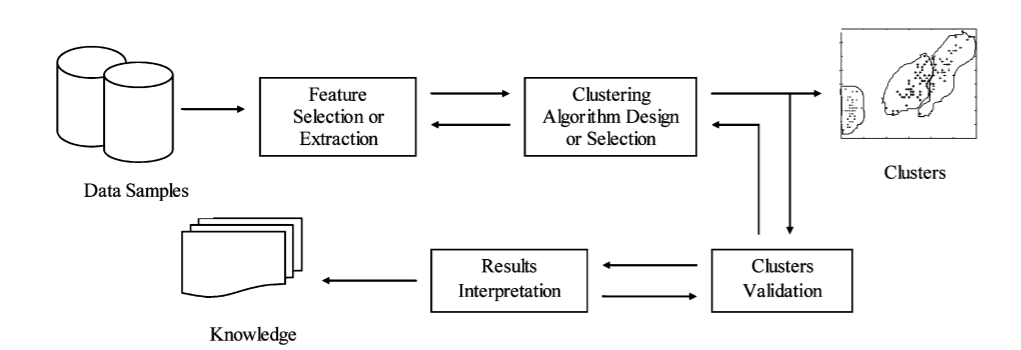
\includegraphics[width=\linewidth]{img/clustering_approach.png}
		\caption{Common clustering procedure.}
	\end{figure}
	In general, a cluster is described by considering its internal homogeneity and the external separation \cite{ClusterHomogeinitySeparation}, meaning that the same cluster should present similar patterns, while patterns in different clusters should not.
	
	Formally, given an input set $X = \{ \pmb{x}_1, ..., \pmb{x_N} \}$ with $\pmb{x}_i \in \mathbb{R}^d$, \textit{hard clustering} attempts to seek a $K$-partition of $X$, $C = \{ C_1, ..., C_K \}$ with $K \leq N$ such that:
	\begin{enumerate}
		 \item $C_i \neq \emptyset$ for $i = 1, ..., K$
		 \item $\cup_{i=1}^{K} C_i = X$
		 \item $C_i \cap C_j = \emptyset$ for each $i, j = 1, ..., K$ with $i \neq j$
	\end{enumerate}
	Therefore, at the end of the procedure, each point in $X$ belongs to a single cluster. In \textit{fuzzy clustering} this constraint is relaxed, and a point $\pmb{x}_i \in X$ can belong to multiple clusters with a certain degree of membership \cite{FuzzyClustering}. Another alternative to hard clustering is \textit{hierarchical clustering}, that repeatedly agglomerates points (or, symmetrically, divides clusters) creating a dendrogram \cite{HierarchicalClustering}.  
	
	The general clustering procedure is depicted in figure \ref{fig:clustering_approach}. The feature selection or extraction step chooses a subset of features from the set of available features. From that subset new features can be generated, for example by using Principal Component Analysis. This step can heavily affect the clustering result. Then, one or more clustering algorithms must be selected often along with a proximity measure (e.g. the Euclidean distance). Note that there isn't any clustering algorithm that is capable of solving all types of problems \cite{ImpossibleTheoremForClustering}. Finally, each clustering algorithm must be objectively validated, and the results interpreted.
	
	In the context of workload characterization (see section \ref{ssec:workload_characterization}) we are interested in hard clustering methods to automatically group workloads. \\
	A well-known clustering method is $k$-means, that partitions $X$ into $k \leq |X|$ clusters $C_1, ..., C_k$ by finding:\\\\
	\centerline{
	$
	\underset{C_1, ..., C_k}{\mathrm{argmax}} \, \sum_{i=1}^{k} \underset{{\pmb{x} \in S}}{\sum} || \pmb{x} - \pmb{\mu}_i ||^2
	$
	} \\\\
	where $\pmb{\mu}_i$ is the \textit{centroid} of cluster $C_i$, and a point $\pmb{x}$ belongs to the cluster having the closest centroid. In order to effectively initialize the value of $\mu_i$, $k$-means++ can be used \cite{kmeans++}. $k$-means requires the number of clusters to be given as input.
	
	Mean shift \cite{MeanShift} is another centroid-based clustering procedure that at each iteration moves the points towards the direction of maximum density by using a kernel function $K(x_i, x)$ (e.g. a Gaussian kernel) that controls the direction of the movement $m(x)$:\\\\
	\centerline{
		$
		m(x) = \frac{\sum_{x_i \in N(x)} K(x_i - x)x_i}{\sum_{x_i \in N(x)} K(x_i - x)}
		$
	} \\\\
	where $N(x)$ is the neighborhood of $x$. The algorithm stops on convergence, i.e. when points cannot further be moved or the movement is below some threshold $\epsilon$. Unlike $k$-means, mean shift doesn't require to know the number of clusters, but it must be provided with a bandwidth parameter that determines the size of the neighborhood $N(x)$. Such bandwidth can be estimated using nearest neighbors.
	
	OPTICS \cite{OPTICS} is a density-based approach that requires two parameters: the minimum number of points required to form a cluster, and the radius $\epsilon$ to consider when forming clusters. OPTICS is very data-efficient for small values of $\epsilon$, and can be used for outlier detection as it doesn't necessarily need to assign a cluster to each point.
	
	Finally, Gaussian Mixture Models (GMM) \cite{MixtureModels} provide a probabilistic approach to clustering by estimating $k$ Gaussian distributions via Expectation-Maximization . The expectation step calculates the probability that a point $\pmb{x}_i$ belongs to the cluster $C_j$, and the maximization step updates the parameters (mean and covariance matrix) of the distributions representing the clusters in order to maximize the log-likelihood function. This process is repeated until convergence. To do so, GMM require to be given the number of components (i.e. clusters) and the covariance type. When compared to $k$-means, the advantage of GMM is that it is not limited to spherical-shaped clusters.
	
	When evaluating the quality of a clustering $C=\{C_1, ..., C_k\}$, the Silhouette coefficient \cite{SilhouetteCoefficient} computes a score representing how well-separated the clusters are. Similarly, the Bayesian Information Criterion \cite{BayesianInformationCriterion} is an alternative applicable to GMM. These scores can be used to choose the number of clusters to be found or method-specific parameter.
	
	\subsection{Forecasting } \label{sec:forecasting}
	Forecasting is a common data science task that makes use of temporal data \cite{ForecastingSurvey} to help organizations with capacity planning, goal setting, and anomaly detection. It is required in many situations: for example, deciding whether to build another warehouse in the next five years requires forecasts of future demand, and scheduling staff in a call center next week requires forecasts of call volumes.
	
	The first successful forecasting methods have been proposed around \textit{1950}, some of them being Exponential Smoothing \cite{ExponentialSmoothingHoltCharles} and ARIMA \cite{ForecastingBoxJenkins}, which originated a wide variety of derived techniques \cite{25YearsForecasting}. In the big-data era, where companies have huge numbers of time series each with their own characteristics, traditional techniques have shown some limitations due to specific model requirements (section \ref{sssec:exponential_smoothing} and \ref{sssec:arma}), model inflexibility, necessity of manual feature engineering, lack of automation, difficulties of dealing with missing data, and lack of well-performing multivariate models \cite{25YearsForecasting}.\\
	Recent developments have seen pure deep learning models joining the fields with inconsistent performance \cite{DeepLearningForecastingSurvey}, but highlighting the possibility of exploiting huge datasets in order to learn a single global model capable of recognizing complex and sometimes shared time series patterns. Other recent deep learning research achievements, especially in the natural language processing domain \cite{RNNLSTM, seq2seq, EncoderDecoder}, have inspired promising models \cite{DeepAR, DeepState, DeepLearningForecastingSurvey}, some of them having an hybrid architecture that utilizes both statistical and machine learning (ML) features \cite{MAKRIDAKIS2018802, GluonTS}. 
	Interestingly, the winner of the 2018 M4 competition \cite{MAKRIDAKIS2018802} was a combination of Exponential Smoothing and deep learning \cite{UberHybridES}, while the top-performing submissions of the 2020 M5 competition \cite{M5Competition}, where most of the time series have some kind of correlation and share frequency and domain, cross-learning ML models have shown their potential with the top-performing submissions using a weighted average of several pure ML models.\\
	Other methods, such as the one proposed by Prophet \cite{FacebookProphet}, provide an analyst-in-the-loop approach suggesting that by injecting domain-specific knowledge into the model it's still possible to outperform fully automated approaches, especially with small amounts of data.\\
	Nevertheless, Artificial Neural Network (ANN) based models have only recently started overtaking simpler classical models \cite{MAKRIDAKIS2018802, M5Competition} opening a set of inspiring possibilities, and the market has seen big companies developing their own solutions \cite{FacebookProphet, GluonTS, MicrosoftSSA, UberHybridES} highlighting the necessity for the businesses of better forecasting techniques.
	
	Despite the forecasting importance, there are still serious challenges associated with producing reliable and high quality forecasts: time series often have long term dependencies with nonlinear relationships.  Moreover, the quality of forecasts are heavily affected by model selection, model tuning, and covariates (e.g. dynamical historical features) selection, where the data scientist has to manually inspect data and inject domain knowledge into the model \cite{DeepLearningForecastingSurvey, FacebookProphet}.\\
	The necessity of tailored forecasting models comes from the fact that time series can be very different from each other, exhibiting complex patterns and relationships with other time series and data in general. 
	
	Nevertheless, time series can often be seen as a composition of a trend, a seasonal pattern, and a cycle \cite{ForecastingHyndmanAthanasopoulos}.
	A trend exists if there is a long-term increase or decrease in the data, which can be linear or not, and can be subject to changes that increase or decrease the trend.
	A seasonal pattern occurs when a time series is affected by seasonal factors like the hour of the day or the day of the week, with fixed and known frequency.
	Finally, a cycle occurs when data rises and falls without a fixed frequency, e.g. due to economic conditions.  Cycles are usually longer than seasonal patterns and have more variable magnitudes.
	
	\begin{figure}
	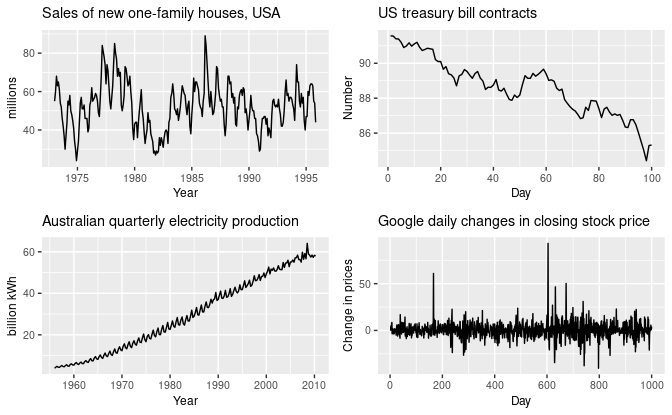
\includegraphics[width=\linewidth]{img/sota_ts_components.png}
	\caption{Four time series examples. Top left: seasonality and cycle; top right: trend only; bottom left: trend and seasonality; bottom right: random fluctuations}
	\end{figure}
	
	Trend and cycles are usually combined into a single trend-cycle component, often referred as trend for simplicity.
	Therefore, we can think of a time series as a combination of a trend-cycle component, a seasonal component, and a remainder component containing anything else in the time series.
	By assuming additive decomposition we can write:\\\\
	\centerline{$y_t = S_t + T_t + R_t$}\\\\
	where $y_t$ is the time series, $S_t$ the seasonal component, $T_t$ the trend component, and $R_t$ the remainder component, all at period $t$. When considering multiplicative decomposition, which occurs when the variation of the trend or of the seasonal component is proportional to the time series level, we can write: \\\\
	\centerline{$y_t = S_t * T_t * R_t$}\\\\
	To obtain such decomposition the Seasonal and Trend decomposition using Loess(STL) \cite{STL} can be applied, leading to the separation of trend, seasonality, and remainder as shown in figure \ref{fig:stl}.
	\begin{figure}
		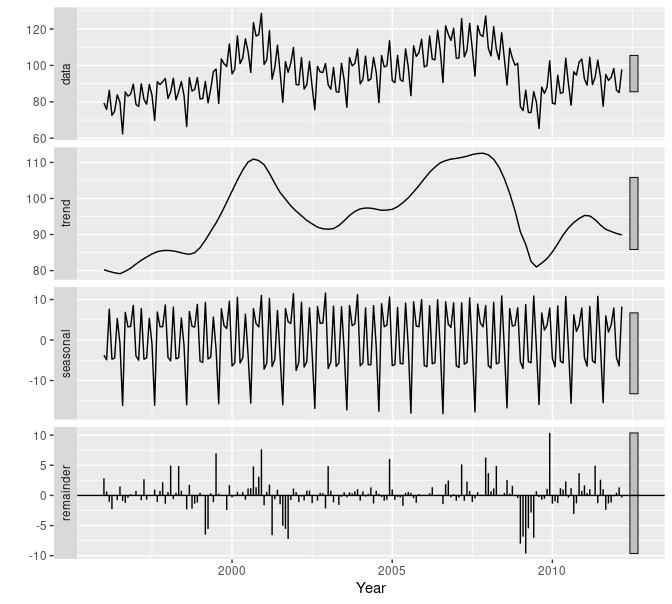
\includegraphics[width=\linewidth]{img/sota_ts_additive_decomposition.png}
		\caption{Additive decomposition of a time series using STL}
		\label{fig:stl}
	\end{figure}
	
	Given this background, let $Z=\{ z_{i, 1:T_i} \}_{i=1}^{N}$ be a  set of $N$ univariate time series where $z_{i, 1:T_i} = (z_{i,1}, z_{i,2}, ..., z_{i,T_i})$ and $z_{i,t} \in \mathbb{R}$ is the value of the $i$-th time series at time $t$. The time series in $Z$ may have different sampling frequencies, can start at different times, and may have missing values. Furthermore, let $X=\{\pmb{x}_{i, 1:T_i+\tau} \}_{i=1}^{N}$ be a set of associated, time-varying covariate vectors with $\pmb{x}_{i,t} \in \mathbb{R}^D$ being any useful information that must be known before computing the forecast up to time $T_i + \tau$ (e.g. a holiday flag).\\
	The goal of forecasting \cite{ForecastingHyndmanAthanasopoulos} is to predict the probability distribution of future values $z_{i,T_{i}+1:T_i+\tau}$ given the past values $z_{i, 1:T_i}$, the covariates $\pmb{x}_{i, 1:T_i + \tau}$, and the model parameters $\Phi$:
	\begin{equation} \label{eq:forecasting}
		p(z_{i,T_{i}+1:T_i+\tau} | z_{i, 1:T_i}, \pmb{x}_{i, 1:T_i + \tau}, \Phi)
	\end{equation}
	which, depending on the model, can be reduced to point forecast by considering the mean (e.g. $\mu$ if the model uses a Gaussian distribution), the median, or by drawing Monte Carlo samples to approximate the mean. The choice between probabilistic and point forecast depends on the application: probabilistic forecast can be used for anomaly detection or when the task has an asymmetric cost for over and under-predicting. \\
	Equation \ref{eq:forecasting} is a supervised learning problem where the model structure is usually fixed upfront and we want to learn the model parameters $\Phi$ using an optimization method such as maximum likelihood estimation.
	
	Univariate models learn the model parameters $\Phi$ for each individual time series, while multivariate models are capable of learning a single global model for multiple time series by sharing the parameters.\\
	As noted by the latest M5 competition \cite{M5Competition}, nowadays time series models are typically sufficient for identifying and capturing their historical data pattern, i.e. level, trend, and seasonality. However, relying solely on historical data fails to effectively account for the effects of holidays and special events. Moreover, such factors can affect historical data, leading to distorted time series and consequently models. In such settings, the information from exogenous/explanatory variables, i.e.  the covariates $\pmb{x}_{i, 1:T_{i+\tau}}$, becomes of critical importance to improve accuracy; in fact, recent models such as the ones discussed later \cite{FacebookProphet, DeepAR, DeepState} allow the inclusion of these kind of variables.
	
	Time series models can be categorized as generative and discriminative \cite{DiscriminativeGenerativeModels} (table \ref{table:generativediscriminative}):
	\begin{table*}\centering 
		\ra{1.3}
		\begin{tabular}{@{}rcr@{}}\toprule
			Category & Modeling\\
			 \midrule
			 Generative & $p(z_{i,1:T_i+\tau} | \pmb{x}_{i, 1:T_i + \tau}, \Phi)$\\
			 Discriminative &  $p(z_{i,T_{i}+1:T_i+\tau} | z_{i, 1:T_i}, \pmb{x}_{i, 1:T_i + \tau}, \Phi)$\\
			\bottomrule
		\end{tabular}
		\caption{Forecasting models} \label{table:generativediscriminative}
	\end{table*}
	generative models assume that time series data is generated by an unknown stochastic process with some parametric structure of parameters $\Phi$ given the covariates $X$, while discriminative models model the conditional distribution for a fixed horizon $\tau$. Discriminative models are typically more flexible since they make less structural assumptions \cite{GluonTS}.
	
	
	\subsubsection{Exponential Smoothing} \label{sssec:exponential_smoothing}
	Exponential smoothing \cite{ExponentialSmoothingHoltCharles} is one of the oldest forecasting techniques that belongs to the generative models class. It is a simple and lightweight state-space model that smooths random fluctuations by using declining weights on older data, it's easy to compute and requires minimum data.
	The simplest form of exponential smoothing assumes that all past observations have equal importance:\\\\
	\centerline{$\hat{y}_{T+1} = \frac{1}{T} \sum_{t=1}^{T}y_t$}\\\\
	where $\hat{y}_{T+1}$ is the forecasted value at time $T+1$ knowing past values up to time $T$. By introducing decaying weights, the formula becomes:\\\\
		\centerline{$\hat{y}_{T+1} = A(y_T + B y_{T-1} + B^2 y_{T-2} + B^3 y_{T-3} + ...)$ }\\\\
	where $A \in [0,1]$ and $B=1-A$, $A$ can attenuate the effect of old observations. The formula can be recursively applied to obtain observation at $T+k$, $k>1$. \\
	Exponential smoothing has been extended to take into consideration linear trend and seasonality \cite{ExponentialSmoothingHoltCharles}. The trend can be approximated applying the same equation above on the time series $z_t = y_t - y_{t-1}$ while to model seasonality its period must be known beforehand.\\
	Note that due to its nature the forecasts produced by Exponential Smoothing will lag behind the actual trend.
	
	A more complex state-space approach, called Innovation State Space Model (ISSM) \cite{ExponentialSmoothingStateSpace}, has been proposed to add a statistical model that describes the data generation process, therefore providing prediction intervals. ISSM maintains a latent state vector $\pmb{l}_t$ with recent information about level, trend and seasonality which evolves over time adding a small innovation at each time step (i.e. the Gaussian noise):\\\\
	\centerline{
	$
	\pmb{l}_t = F_t \pmb{l}_{t-1} + \pmb{g}_t \epsilon_t,\; \epsilon_t \sim \mathcal{N}(0,1)
	$
	}\\\\
	where $\pmb{g}_t$ controls innovation strength and $F_t$ is the transition matrix. 
	The observations become a linear combination of the current state $\pmb{l}_t$:\\\\
	\centerline{$
	y_{t+1} = \pmb{a}_{t}^T \pmb{l}_t + b_{t} + \nu_t,\; \nu_t \sim \mathcal{N}(0,1)
	$}\\\\
	The ISSM parameters $(F_t, \pmb{g}_t, \pmb{a}_t, b_t, \nu_t)$ are typically learned using the maximum likelihood principle.
	
	\subsubsection{ARMA models} \label{sssec:arma}
	
	ARMA models are Auto-Regressive models with a Moving-Average component, they provide a complementary approach to Exponential Smoothing and they belong to the generative models class. \\
	The Auto Regressive component of order $p$, $\text{AR}(p)$, predicts the next value using a linear combination of $p$ previous known values, while the Moving Average component of order $q$, $\text{MA}(q)$, takes into consideration the average and the last $q$ differences between the predicted and the actual value.  When combined, they form an ARMA$(p, q)$ model:\\\\
	\centerline{$\hat{y}_{t} = \text{ARMA}(p, q) = \text{AR}(p) + \text{MA}(q)  = \sum_{i=1}^{p}\phi_i y_{t-i} + \mu + \epsilon_t + \sum_{i=1}^{q}\theta_i \epsilon_{t-i} $}\\\\
	Unfortunately, ARMA requires the time series to be stationary, i.e. without trends and seasonality. To make a time series stationary and apply ARMA models, Box and Jenkins \cite{BoxJenkins} proposed an approach by: (1) providing guidelines for making the time series stationary, (2)  suggesting the use of autocorrelations and partial autocorrelation for determining appropriate values for $p$ and $q$, (3) providing a set of computer programs to identify appropriate values for $p$ and $q$, and (4) estimating the parameters involved. The approach is known as the Box-Jenkins methodology to ARIMA models, where the letter \lq I \rq means ``Integrated'', reflecting the need for differencing the time series to make it stationary. Furthermore, ARIMA can deal with seasonality by applying seasonal differencing, but requires the seasonality period to be known beforehand. This extension is called SARIMA.
	
	The more general SARIMA$(p, d, q, P, D, Q, m)$ model is defined by 7 parameters:
	\begin{itemize}
		\item $p$: trend auto-regression order
		\item $d$: trend difference order
		\item $q$: trend moving average order
		\item $P$: seasonal auto-regressive order
		\item $D$: seasonal difference order
		\item $Q$: seasonal moving average order
		\item $m$: seasonal period steps
	\end{itemize}

	Besides the availability of the well defined 3-steps Box-Jenkins framework, a decent amount of human work was still required to find the right values for these parameters. To tackle this issue many approaches have been developed, some of them being made available only by commercial software.  A well known automated solution has been implemented by \cite{AutoForecasting}, where they make use of unit root tests to find the differencing orders and the Akaike's information criterion (AIC) to select the best combination of $p$, $q$, $P$, and $Q$. AIC introduces a model complexity penalty to avoid overfitting data.\\
	Nevertheless, the number of steps of the seasonal period must still be given by the analyst, although it's often a well known seasonality (e.g. daily, weekly, yearly).
		
	The vector ARIMA (VARIMA) model has been proposed as a multivariate generalization of the univariate ARIMA model, but in general Vector Auto-Regressive (VAR) models tend to suffer from overfitting, providing poor out-of-sample forecasts \cite{25YearsForecasting}.
	
	\subsubsection{Prophet } \label{sssec:prohet}
	Prophet \cite{FacebookProphet} is a solution developed by Facebook that provides an ``analyst-in-the-loop'' approach (figure \ref{fig:analyst_in_the_loop}) and a flexible model that fit a wide range of business time series. The model simplifies the process of adding domain knowledge about the data generation process and reduces the time required to obtain high quality forecasts. Finally, Prophet is able to automatically handle time series with trend changes, multiple seasonality, and holidays effects.
	\begin{figure}
		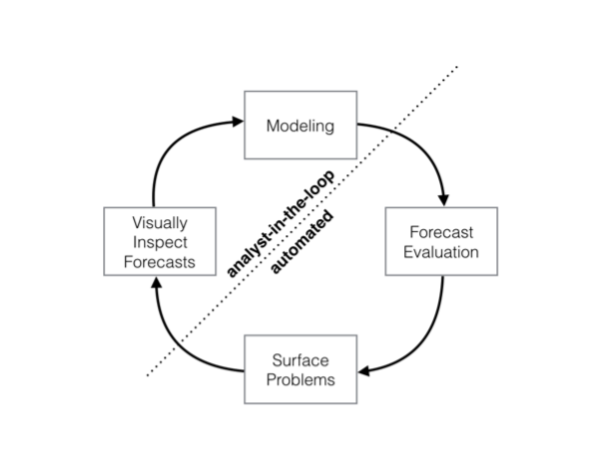
\includegraphics[width=\linewidth]{img/sota_ts_fb_prophet.png}
		\caption{Prophet analyst-in-the-loop approach}
		\label{fig:analyst_in_the_loop}
	\end{figure}
	Prophet model is a Generalized Additive Model (GAM) \cite{GAM} that decomposes trend, seasonalities, and holidays combining them in the following equation:\\\\
	\centerline{$y(t) = g(t) + s(t) + h(t) + \epsilon_t$}\\\\
	where $g(t)$ is the trend function which models non-periodic changes, $s(t)$ is the seasonality function that models periodic changes like daily and weekly seasonality, and $h(t)$ represents the effect of holidays which occur on potentially irregular schedules. Finally, the error term $\epsilon_t$ represents anything not accommodated by the model, which is assumed to be normally distributed. \\
	The GAM formulation can be easily extended to add new components as necessary and it can fit very quickly using optimization methods like L-BFGS \cite{L-BFGS}, making the forecasting problem a curve-fitting problem which allows non-regularly spaced measurements (e.g. due to missing values).\\
	The trend model $g(t)$ can be a saturating growth model capable of dealing with a limited population growth (e.g. the number of subscriptions limited by the population of a country) or a piece-wise linear model.
	The latter has the following form:\\\\
	\centerline{
		$g(t) = (k+\pmb{a}(t)^T\pmb{\delta})t + (m + \pmb{a}(t)^T\gamma)$
	}\\\\
	where $k$ is the growth rate, $\pmb{\delta}$ is the rate adjustments vector, $m$ is the offset parameter, and $\gamma_j$ is set to $-s_j\delta_j$ to make the function continuous.\\
	Therefore, $\pmb{\delta} \in \!R^S$ defines $S$ trend change points occurring at time $s_j$, with $\delta_j$ being the rate adjustment. The rate at time $t$ is $k+\sum_{j:t>s_j}\delta_j$, which is more cleanly defined by a vector $\pmb{a}(t) \in \{0,1\}^S$ such that:\\\\
	\centerline{
		$
		a_j(t) =
		\begin{cases}
			1 & \text{if $t \geq s_j$}\\
			0 & \text{otherwise}
		\end{cases}       
		$
	}\\\\
	that makes the rate at time $t$ be $k + \pmb{a}(t)^T\pmb{\delta}$\\
	The change points $s_j$  can be specified by the analyst or they can be automatically selected by putting a sparse prior on $\pmb{\delta}$, e.g. a Laplace prior.\\
	The seasonality function $s(t)$ is modeled using Fourier series, meaning that a seasonality with period $P$ can be approximated by:\\\\
	\centerline{$s(t) = \sum_{n=1}^{N} (a_n \cos{(\frac{2\pi nt}{P})} + b_n \sin{(\frac{2\pi nt}{P})}) $}\\\\
	which can be automatically estimated finding $2N$ parameters, i.e.\\ $ \pmb{\beta} =  (a_1, b_1, ..., a_N, b_N)$. By choosing $N$, the series can be truncated at different depths allowing to fit seasonal patterns that change more or less quickly, possibly leading to overfitting. Finally, the initialization $\pmb{\beta} \sim \mathcal{N}(0, \sigma^2)$ allows to impose a prior on the seasonality by choosing $\sigma$. \\
	The holiday model $h(t)$ can deal with predictable shocks that cannot be modeled by a smoothed Fourier series.  An example could be the increase of units sold during Easter, which doesn't falls a specific day. An analyst can provide a list of dates of interest $D_j$ for each holiday $j$, so the holiday model becomes:\\\\
	\centerline{$h(t) = Z(t) \pmb{\kappa}$}\\\\
	with $Z(t) = [ \mathbf{1} (t \in D_1), ..., \mathbf{1} (t \in D_L)] $ and $\pmb{\kappa}$ initialized as $\pmb{\kappa} \sim \mathcal{N}(0, v^2)$, like it was done with seasonality.\\
	The Prophet solution is capable of achieving lower prediction errors when compared to traditional methods like Exponential Smoothing and ARIMA, with very quick fitting time.
	
	\subsubsection{ML models}
	The forecasting field has seen past practitioners proposing novel Neural Networks (NN) architectures that could not be considered competitive against simpler univariate statistical models. However, we are now living in the Big Data era: companies have gathered huge amounts of data over the years containing important information about their business patterns, unlocking the possibility of learning effective multivariate models. Big data in the context of time series doesn't necessarily mean having single time series with with a lot of historical data, but it rather means that there are many related time series from the same domain \cite{RNNForecasting}. In such context, models capable of learning from multiple time series have emerged \cite{M5Competition} outperforming traditional ones while alleviating the time and labor intensive manual feature engineering by making no explicit assumptions on data and therefore being more flexible when compared to traditional techniques such as ARIMA and Exponential Smoothing.
	
	All recent successful models are based on Recurrent Neural Networks (RNN) \cite{RNN, RNNForecasting}, which demonstrated state-of-the-art performance in various applications handling sequential data like text, audio, and video where some kind of state must be kept while processing. RNNs can be combination of recurrent units like Long Short-Term Memory (LSTM) and Gated Recurrent Unit (GRU) (see figure \ref{fig:lstmgru}). 
	\begin{figure}
		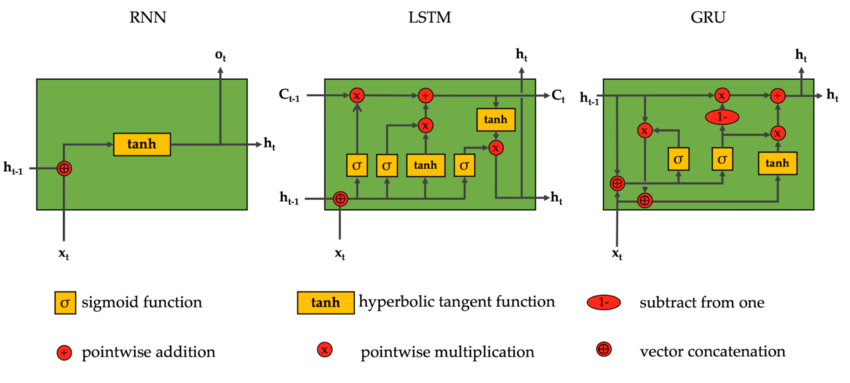
\includegraphics[width=\linewidth]{img/rnns.png}
		\caption{Architecture of an Elman recurrent unit, LSTM, and GRU. The output at step $t-1$ influences the output at step $t$.}
		\label{fig:lstmgru}
	\end{figure}
	By using recurrent edges connecting adjacent time steps (i.e. feedback loops), RNNs introduce the notion of time to the model: at time step $t$ the network receives the current input $\pmb{x}^{(t)}$ plus the previous network state $\pmb{h}^{(t-1)}$ producing a new context $\pmb{h}^{(t)}$ (often called hidden state) and eventually an output $\pmb{o}^{(t)}$.
	The context acts as a memory of what the network has seen so far and influences the output, unlocking a stateful decision making.\\
	However, the first recurrent unit (i.e. the Elman recurrent unit) suffered from the vanishing/exploding gradient problem \cite{VanishingGradient} which causes the inability of carrying long-term dependencies. To address this shortcoming, the Elman recurrent unit has been extended leading to improved variants such as LSTM and GRU.
	
	LSTM uses two components for its state: the hidden state and the internal state, containing short-term and long-term memory respectively. Furthermore, LSTM introduces a gating mechanism made of an input, forget, and output gate used to filter what should or should not be kept of the state in the next step (for example, to disable the output contribution to the LSTM state just set the output gate to zero). GRU is a simpler version of LSTM with fewer gates (update and reset) which allows faster computations and is less prone to overfitting due to the lower number of parameters.
	
	Recurrent units (e.g. LSTM, GRU) can constitute RNNs in various types of architectures, depending on the application: a many-to-one (or sequence-to-vector) architecture can be used for sentiment classification, one-to-many (or vector-to-sequence) for for music generation, and many-to-many (or sequence-to-sequence) for machine translation (see figure \ref{fig:rnn_architectures}).
	\begin{figure}
		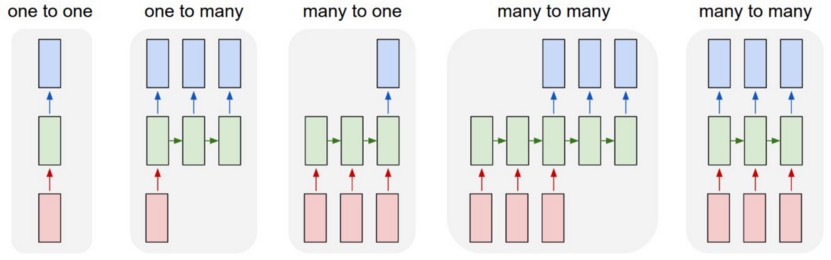
\includegraphics[width=\linewidth]{img/rnn_architectures.png}
		\caption{RNN architectures. Red rectangles are input vectors, blue rectangles are output vectors, and green rectangles are recurrent units such as LSTM or GRU which share the same weights while their state evolves from left to right.}
		\label{fig:rnn_architectures}
	\end{figure}

	To obtain such architectures a single LSTM can be used, in that case the green LSTM in figure \ref{fig:rnn_architectures} is unfolded such that in the whole processing of the input the same weights are used, while the internal state of the LSTM evolves.	Nevertheless, multiple LSTMs can be stacked together such as in figure \ref{fig:stacked_lstm} composing multiple layers and increasing the expressiveness of the network.
	\begin{figure}
		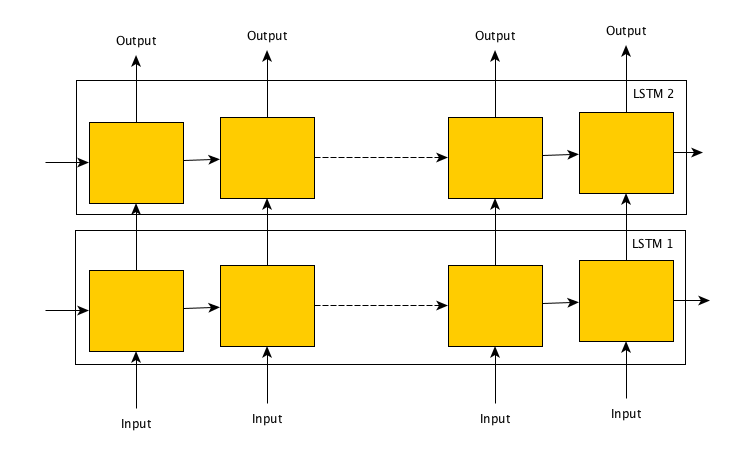
\includegraphics[width=\linewidth]{img/stacked_lstm.png}
		\caption{2-layers stacked LSTMs. }
		\label{fig:stacked_lstm}
	\end{figure}
	Usually when forecasting the size $d$ of the output (or the internal state of an LSTM) doesn't match the dimension of the forecasting horizon $H$. In such cases, another neural layer is added to map $\pmb{o}^{(t)} \in \mathbb{R}^d$ to the forecast $\hat{\pmb{y}}^{(t)} \in \mathbb{R}^H$. This neural layer is trained together with the LSTM, with the loss (e.g. the forecasting error $|\hat{y} - y|$) being calculated per each time step and accumulated until the end of the time series after which backpropagation through time is executed.
	
	Forecasting requires a many-to-many architecture: the input is a sequence, i.e. a time series, and the output is another sequence that is a continuation of the input sequence, i.e. a forecast of horizon $H$. In such context, the Sequence to Sequence (S2S) \cite{seq2seq} models have proven to be successful. S2S models are made of two RNNs: an encoder followed by a decoder, as shown in figure \ref{fig:seq2seq}.
	\begin{figure}
		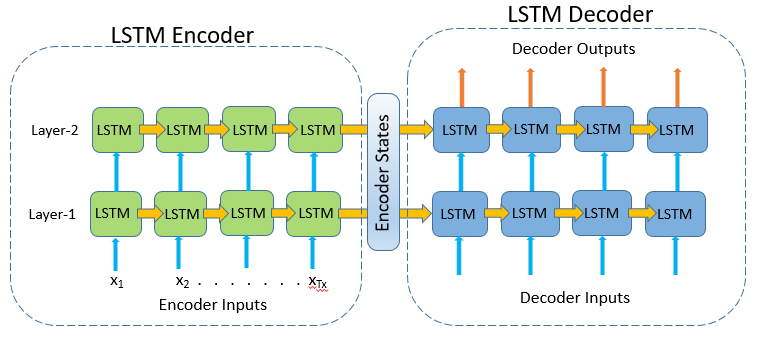
\includegraphics[width=\linewidth]{img/seq2seq.png}
		\caption{Sequence to sequence model}
		\label{fig:seq2seq}
	\end{figure}
	 The encoder is used to extract features from known time series data in order to produce a context vector (e.g. the LSTM hidden state) that is given as input to the decoder to produce forecasts. Examples of models based on S2S are DeepAR \cite{DeepAR} and Multi-Horizon Quantile Recurrent Forecaster \cite{MQCNN}, explained later. By defining an encoder and a decoder, a model is allowed to see a limited amount of past values and can predict a fixed horizon, which means that any context and prediction length change requires re-training. 
	 
	 The decoder at time step $t+1$ can receive as input the prediction made at step $t$, but many forecasting problems have long periodicity (e.g. 365 days) and may suffer memory loss during forward propagation. To overcome the long-term dependency issue \cite{NARX} proposed a recurrent unit which computes a hidden state $\pmb{h}^{(t)}$ not only based on previous state $\pmb{h}^{(t-1)}$ but also a specific set of other past states (e.g. $(\pmb{h}^{(t-2)}), ..., \pmb{h}^{(t-D)})$) facilitating the ability of keeping long dependencies. This technique is called skip-connection. However, the naive alternative adopted by \cite{DeepAR, MQCNN} obtains the same effect by directly feeding past time series values $(y_{t-1}, ..., y_{t-D})$ as feature inputs to the decoder.
	
	More generally, the idea of feeding both time-dependent and time-independent features as input (often called exogenous variables), along with the time series data points, has proven to be successful: when dealing with huge datasets, assigning time-independent (or static) features such as the category of the time series (e.g. ``clothing'' in the context of shopping) allow the model to learn both global and category-specific patterns, while time-dependent (or dynamic) features like day of week, holidays, and relevant events allow the model to learn and distinguish seasonality patterns from one-shot events like anomalies, reducing the risk of overfitting. However, such dynamic features must be known beforehand when computing forecasts, and in some contexts they can be used to make conditional forecasts, e.g. "\textit{How many units of product X will I sell if I set the price to Z?}".
	
	The usage of such combination of features facilitates the learning of a global model exploiting information from many time series simultaneously. For NNs this means that weights are learned globally, but the state is maintained for each time series. Furthermore, the global model can be used to forecast time series that have never been seen during training and lack of data, as the model can still use patterns learned from the training set.
	
	
	
	
	% TODO introduction about RNNs - characteristics e.g. of LSTM - see https://arxiv.org/pdf/1705.04378.pdf , background of https://arxiv.org/pdf/1703.04691.pdf
	\subsubsection{DeepAR } \label{sssec:deepar}
	DeepAR \cite{DeepAR} is a discriminative model capable of probabilistic forecasts in the form of Monte Carlo samples, it is based on Sequence to Sequence (S2S) \cite{seq2seq} and can learn a global model from multiple time series.\\
	Alongside with a model, DeepAR proposes a solution to the issue of dealing with time series having very different magnitudes, which are known to ruin the learning of an effective global model reducing the effectiveness of normalization techniques on some datasets \cite{DeepAR}.
	
	DeepAR goal is to model the conditional distribution\\\\
	\centerline{
	$
	P(\pmb{z}_{i, t_0:T} | \pmb{z}_{i, 1:t_0-1}, \pmb{x}_{i, 1:T})
	$
	}\\\\
	where $\pmb{z}_{i, t_0:T} = [z_{i,t_0}, z_{i, t_0+1}, ..., z_{i, T}]$ is the future (or prediction range), $\pmb{z}_{i, 1:t_0-1}$ is the past (or conditioning range), and $\pmb{x}_{i, 1:T}$ are covariates that must be known for all time points.
	
	DeepAR assumes that its distribution $Q_{\Theta}(\pmb{z}_{i, t_0:T} | \pmb{z}_{i, 1:t_0-1}, \pmb{x}_{i, 1:T})$ consists of a product of likelihood factors:\\\\
	\centerline{
	$
	Q_{\Theta}(\pmb{z}_{i, t_0:T} | \pmb{z}_{i, 1:t_0-1}, \pmb{x}_{i, 1:T}) 
	= \prod_{t=t_0}^{T} Q_{\Theta}(z_{i, t} | \pmb{z}_{i, 1:t-1}, \pmb{x}_{i, 1:T})
	= \prod_{t=t_0}^{T} \textit{l}(z_{i,t} | \theta(\pmb{h}_{i,t}, \Theta))
	$
	}\\\\
	which is parametrized by the output $\pmb{h}_{i,t}$ of an autoregressive RNN
	\begin{equation} \label{eq:autoregressive_rnn}
		\pmb{h}_{i,t} = \textit{h}(\pmb{h}_{i,t}, \pmb{z}_{i, t-1}, \pmb{x}_{i, t}, \Theta )
	\end{equation}
	where \textit{h} is implemented by multi-layer RNN with LSTM cells, meaning that $\pmb{h}_{i,t}$ is given by the internal state of the LSTMs as shown in figure \ref{fig:deepar}. \\
	$\textit{l}(z_{i,t} | \theta(\pmb{h}_{i,t})$ is the likelihood of a fixed distribution (e.g. Student's t-distribution) whose parameters are given by a function $\theta(\pmb{h}_{i,t}, \Theta)$ of the network output $\pmb{h}_{i,t}$.
	\begin{figure}
		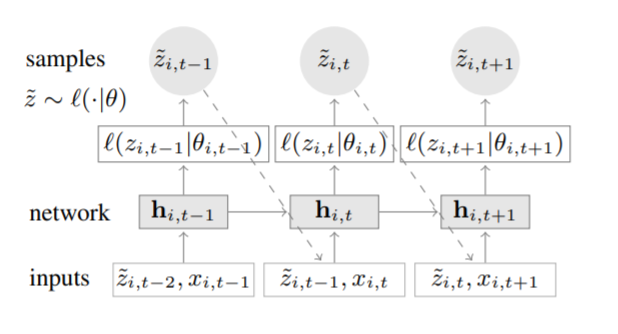
\includegraphics[width=\linewidth]{img/deepar.png}
		\caption{DeepAR decoder network}
		\label{fig:deepar}
	\end{figure}
	The model is autoregressive and recurrent as it uses the previous output $\tilde{z}_{i,t}$ and state $\pmb{h}_{i,t}$ as input, which potentially means that prediction errors at time $t$ will negatively affect predictions at time $t>1$. \\
	The initial state $\pmb{h}_{i,t_0-1}$ of the decoder shown in figure \ref{fig:deepar} is obtained using an encoder with the same architecture and weights that computes equation \ref{eq:autoregressive_rnn} for $t = 1, ..., t_0-1$. The forecasts $\tilde{\pmb{z}}_{i, t_0:T}$ are obtained by sampling $\tilde{z}_{i,t} \sim l(\cdot | \theta(\pmb{h}_{i,t}, \Theta))$, where $\theta(\pmb{h}_{i,t}, \Theta))$ are the parameters (e.g. mean and variance) of the distribution fixed during training and are directly predicted by the decoder network.
	
	The likelihood $l(z | \theta)$ determines the noise model and should match the statistical properties of the data: a Gaussian likelihood can be used for real-valued data, a beta likelihood for data in the unit interval, and a negative-binomial likelihood for positive count data. For example, the Gaussian likelihood is parametrized using its mean and standard deviation, i.e. $\theta = (\mu, \sigma)$ where $\mu$ is obtained with an affine function of the network output $\pmb{h}_{i,t}$ and the standard deviation is obtained by applying an affine transformation followed by a softplus activation to ensure $\sigma > 0$,
	Therefore, each likelihood with parameters $\theta$ requires a mapping from the decoder state $\pmb{h}_{i,t}$ to $\theta$ whose parameters are learned by the network.
	
		Without any modification, in order to handle different scales the network should learn to scale the input to an appropriate range and then invert the scaling. As the network has a limited operating range and some datasets exhibit a power-law of scales (such as the Amazon dataset of \cite{DeepAR}), this issue was addressed by scaling the input values (e.g. $\tilde{z}_{i, t}$ and $z_{i,t}$) using an item-dependent factor $\nu_i$. Then, before drawing samples from the distribution, the output of the network (e.g. the mean $\mu$ of the Gaussian) is multiplied by the scale. The scaling factor $\nu$ is set to be the average value of the time series: $\nu_i = 1 + \frac{1}{t_0} \sum_{t=1}^{t_0} z_{i,t}$. Finally, rather than training the network choosing random time series from the dataset, the probability of choosing a time series is proportional to its scale factor $\nu_i$: by non-uniformly sampling during training, imbalanced datasets with fewer large scale time series are used more effectively.
		
	
	\subsubsection{DeepState } \label{sssec:deepstate}
	DeepState \cite{DeepState} is a generative model that combines state space models \cite{ExponentialSmoothingStateSpace} with deep learning. The idea is to use a latent state $\pmb{l}_t \in \mathbb{R}^D$ to encode time series components such as level, trend, and seasonality patterns, and parametrize the linear state space model (SSM) by using a recurrent neural network (RNN) whose weights are learned jointly from multiple time series and covariates. \\
	The main advantage of SSM is that the model is easily interpretable, but when used with traditional models such as ARIMA and Exponential Smoothing it results in an univariate model that still requires a lot of human work that cannot be easily recycled for other time series.
	DeepState solves this issue by using neural networks to learn a global model from multiple time series without making strong assumptions and reducing the human effort, and solving the common interpretability issue of neural networks by fusing them with SSMs.
	
	The goal of DeepState is to produce probabilistic forecasts for each time series $i=1,...,N$ given the past:\\\\
	\centerline{
	$
	p(\pmb{z}_{i, T_i+1:T_i+\tau}| \pmb{z}_{i, 1:T_i}, \pmb{x}_{i, 1:T_i+\tau}; \Phi)
	$
	}\\\\
	where $\pmb{z}_{i, T_i+1:T_i+\tau}$ are the $\tau$ future values, $ \pmb{z}_{i, 1:T_i}$ are the known past values, $\pmb{x}_{i, 1:T_i+\tau}$ are the covariates that must be known beforehand for $t=1,...,T$, and $\Phi$ is the set of learnable parameters of the model (i.e. the RNN).\\
	DeepState makes the assumption that time series are independent of each other when conditioned on the associated covariates $\pmb{x}_{i, 1:T}$. Nevertheless, the model is still able to learn and share patterns across time series as $\Phi$ is shared (and learned) between all of them.
	
	SSMs use a latent state $\pmb{l}_t \in \mathbb{R}^L$ encoding time series components (level, trend, seasonality) that evolves over time with linear transitions at each time step $t$:\\\\
	\centerline{
	$
	\pmb{l}_t = F_t \pmb{l}_{t-1} + \pmb{g }_t \epsilon_t, \;\; \epsilon_t \sim \mathcal{N}(0,1)
	$
	}\\\\
	where $F_t$ is the transition matrix and $\pmb{g }_t \epsilon_t$ is a random innovation component. The latent state can be inspected to check and potentially change the encoded trend and seasonality, and is also used to obtain predictions. For example, considering a linear Gaussian observation model:
	\begin{equation} \label{eq:deepstate}
			z_t = y_t + \sigma_t \epsilon_t, \;\; y_t = \pmb{a}_t^T \pmb{l}_{t-1} + b_t, \;\; \epsilon_t \sim \mathcal{N}(0,1)
	\end{equation}
	with the initial state $\pmb{l}_0 \sim \mathcal{N}(\pmb{\mu}_0, \text{diag}(\pmb{\sigma}_0^2))$, $\pmb{a}_t \in \mathbb{R}^L$, $\sigma_t \in \mathbb{R}_{>0}$, and $b_t \in \mathbb{R}$ varying over time. \\
	Therefore, the state space model of \textit{one} time series is fully described by $\Theta_t = (\pmb{\mu}_0, \pmb{\sigma}_0, \pmb{F}_t, \pmb{g}_ t, \pmb{a}_t, b_t, \sigma_t), \; \forall t > 0$, differing from the classical settings where $\Theta$ doesn't change with time.\\
	To obtain $\Theta_{i,t}$ for the time series $i$, the DeepState model learns a mapping $\Psi$ from the covariates $\pmb{x}_{i, 1:T_i}$ to the parameters $\Theta_{i, t}$:\\\\
	\centerline{
	$
	\Theta_{i,t} = \Psi(\pmb{x}_{i, 1:T}, \theta)
	$
	}\\\\
	that is parametrized from a set of parameters $\theta$ learned jointly from the entire dataset of time series. \\
	More precisely, the mapping $\Psi$ is implemented by the RNN shown in figure \ref{fig:deepstate} having a stacked architecture of LSTM cells. Its parameters $\theta$ are learned by maximizing the likelihood during training.
	\begin{figure}
		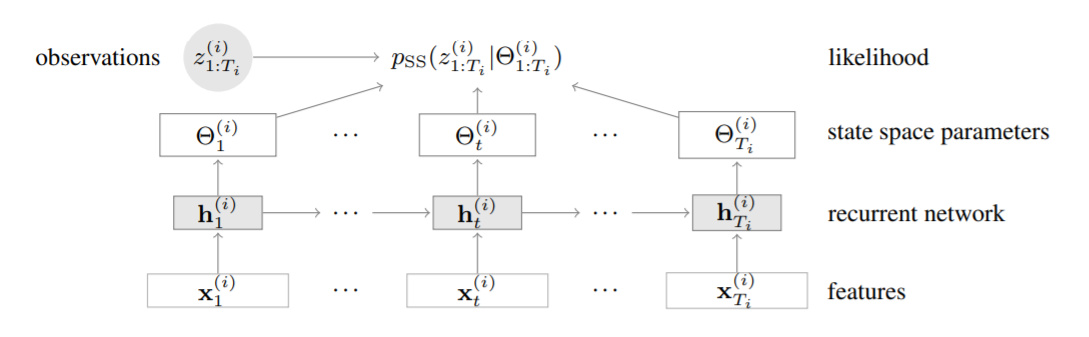
\includegraphics[width=\linewidth]{img/deepstate.png}
		\caption{DeepState network}
		\label{fig:deepstate}
	\end{figure}

	Finally, once the mapping is learned and given $\pmb{x}_{i, 1:T_i}$, the data $\pmb{z}_{i,1:T_i}$ is distributed according to the marginal likelihood:\\\\
	\centerline{
	$
	p(\pmb{z}_{i, 1:T_i} | \pmb{x}_{i, 1:T_i}, \theta)
	= p_{SS}(\pmb{z}_{i, 1:T_i} | \Theta_{i,1:T_i})
	$
	}\\\\
	\centerline{
		$
		= p(z_{i,1} | \Theta_{i,1}) \prod_{t=2}^{T}p(z_{i,t} | z_{i, 1:t-1}, \Theta_{i, 1:t})
		$
	}\\\\
	\centerline{
		$
		= \int p(\pmb{l}_0) [\prod_{t=1}^{T_i} p(z_{i,t} | \pmb{l}_t)p(\pmb{l}_t | \pmb{l}_{t-1})] d\pmb{l}_{0:T_i}
		$
	}\\\\
	that is analytically tractable in the linear-Gaussian case.\\
	To produce a forecast, the posterior of the last latent state $p(\pmb{l}_T | z_{i, 1:T_i})$ is computed using the observations $z_{i, 1:T_i}$, then the RNN is fed with the covariates $x_{i, 1:T_i+\tau}$ (see figure \ref{fig:deepstate2}) while the transition equation is recursively applied, drawing Monte Carlo samples using equation \ref{eq:deepstate}.
	\begin{figure}
		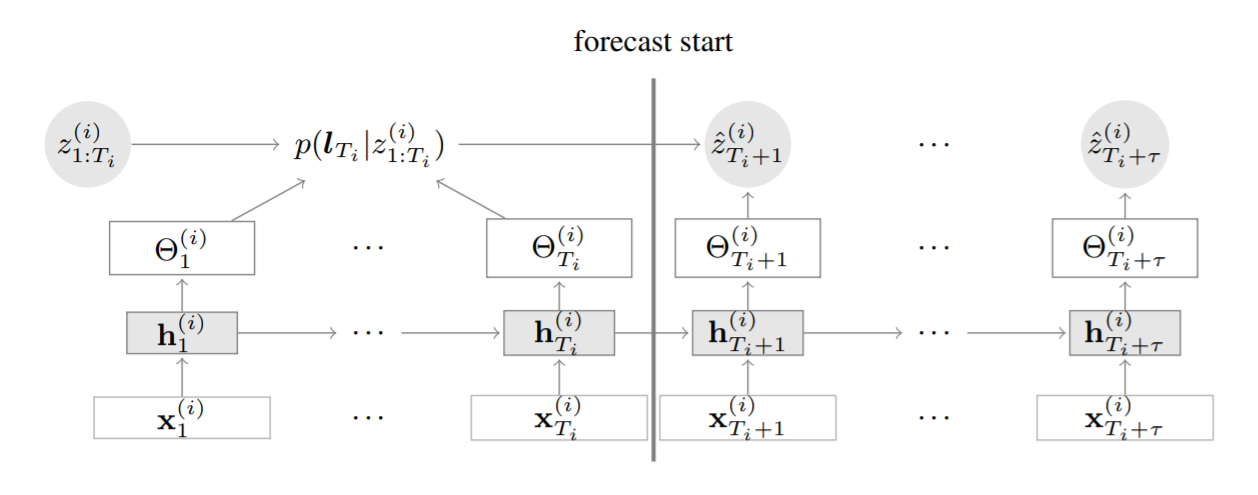
\includegraphics[width=\linewidth]{img/deepstate2.png}
		\caption{DeepState forecast illustration}
		\label{fig:deepstate2}
	\end{figure}

	\subsubsection{Multi Quantile Recurrent Forecaster } \label{sssec:mqcnn}
	Multi Quantile Recurrent Forecaster (MQCNN) \cite{MQCNN} is a Sequence-to-Sequence RNN-based model capable of producing multi-horizon quantile forecasts.\\
	\cite{MQCNN} proposes a forking-sequences approach that improves the training stability and performance of encoder-decoder architectures by efficiently training on all time points where a forecast could be created. Furthermore, the model can be used with different encoders, but the best results were achieved using a CNN-based encoder.
	
	To train a quantile regression model for a quantile $q \in [0, 1]$ the loss of a single forecasted value is given by:\\\\
	\centerline{
	$
	L_q(y, \hat{y}) = q \max(0, y-\hat{y}) + (1-q) \max(0, \hat{y} - y)
	$
	}\\\\
	where by setting $q=0.5$ the model will be trained to simply predict the median. Note that by predicting quantiles the model is robust since it doesn't make distributional assumptions (e.g. like DeepAr \cite{DeepAR}). \\
	Eventually, more quantiles can be considered such that the total loss is given by:\\\\
	\centerline{
	$
	\sum_{t\in T} \sum_{q\in Q} \sum_{k=1}^K L_q(y_{t+k}, \hat{y}_{t+k}^{(q)})
	$
	}\\\\
	where $T$ contains the forecast creation times, $Q$ the quantiles, and $K$ is the size of the horizon to forecast. Furthermore, different quantiles can be associated with different weights, which could be useful for tasks with an asymmetric cost for over and under-predicting.
	
	The general architecture of a multi-quantile recurrent forecaster is shown in figure \ref{fig:mqforecaster}. 
	\begin{figure}
		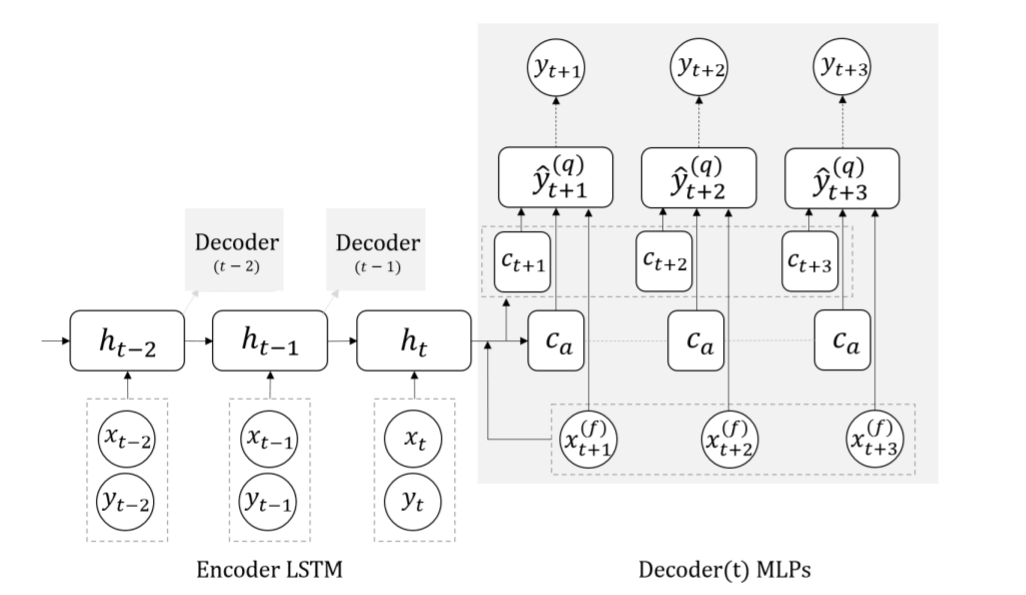
\includegraphics[width=\linewidth]{img/mqcnn.png}
		\caption{Multi-quantile recurrent forecaster architecture}
		\label{fig:mqforecaster}
	\end{figure}
	The encoder is fed with the time series history producing hidden states $h_t$,  then a global neural network summarizes the encoder output into an horizon-agnostic context $c_a$ plus a horizon-specific context $c_{t+k}$ for $k=1,...,K$ using the hidden state $h_t$ and the future covariates $x_{t+1:t+K}$:\\\\
	\centerline{
	$
	(c_{t+1, ..., c_{t+K}, c_a}) = m_G(h_t, x_{t+1:t+K})
	$
	}\\\\
	where each context $c_i$ can have arbitrary dimension. The idea behind this choice is that $c_a$ should capture relevant information that is not time-sensitive, while $c_{t+k}$ carries awareness of the temporal distance between the forecast creation time $t$ and the specific horizon.\\ 
	Then, these contexts are used by a local neural network to compute the quantiles of a specific horizon $t+k$ for each $k=1,...,K$ using the horizon-agnostic context and the horizon-specific context, plus the associated covariates:\\\\
	\centerline{
	$
	(\hat{y}_{t+k}^{(q_1)}), ..., \hat{y}_{t+k}^{(q_Q)}) = m_L(c_{t+k}, c_a, x_{t+k})
	$
	}\\\\
	The local neural network implementing $m_L$ has its parameters shared across all the horizons.
	
	The motivation for replacing the standard RNN-based decoder is that the horizon-specific context should have already captured the flow of temporal information. Furthermore, by not feeding predictions recursively there is no error accumulation and following the forking-sequences training scheme proposed by \cite{MQCNN} the training time is dramatically reduced while the process of updating the gradients is stabilized, leading to better forecasts with a reduced effort.
	
	The encoder is not limited to be a simple LSTM-based RNN: \cite{MQCNN} achieved the best results using a CNN-based encoder made of a stack of dilated causal convolutional layers, similarly to the work done by WaveNet \cite{Wavenet}.\\
	Dilated causal convolutional layers, shown in figure \ref{fig:dilated_cnn}, form long-term connections creating large receptive fields with just a few layers, thus preserving computational efficiency. The result is the so-called MQ-CNN model.
	\begin{figure}
		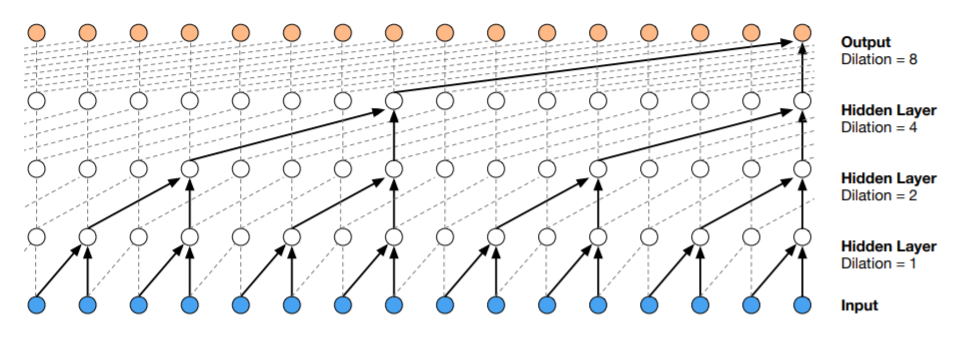
\includegraphics[width=\linewidth]{img/wavenet.png}
		\caption{A stack of dilated causal convolutional layers}
		\label{fig:dilated_cnn}
	\end{figure}
	
	
	\subsection{Workload forecasting } \label{ssec:workload_forecasting}
	% ADD stuff about short term load forecasting (STLF) see https://arxiv.org/pdf/1705.04378.pdf
	The ability of forecasting the workload of an IT system opens the possibility of proactively adapting the system according to the future demand and making smarter decisions, keeping the Quality of Service (QoS) high while reducing the infrastructure costs. This section lists some applications of workload forecasting and how it has been approached.\\
	Recent years have seen companies moving from self-hosted to cloud-hosted  IT services, where a public provider is paid to lend on-demand computing power likewise utilities such as electricity, gas, and water. This paradigm, called cloud computing \cite{CloudComputing}, enabled the possibility of flexibly adapting the capacity of a system according to the demand, potentially heavily reducing the infrastructure costs.  Figure \ref{fig:cloud_vs_traditional_computing} highlights the difference of cloud computing with the traditional paradigm, where to avoid loosing customers the capacity of the system must be able to serve the highest peak of demand, causing an over-provisioning of resources when the demand is low.\\
	\begin{figure}
		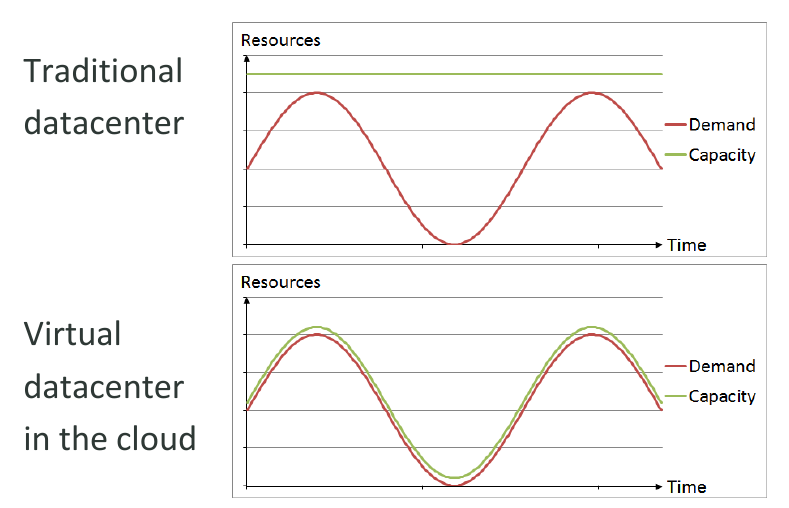
\includegraphics[width=\linewidth]{img/cloud_vs_traditional_computing.png}
		\caption{Cloud vs traditional computing.}
		\label{fig:cloud_vs_traditional_computing}
	\end{figure}
	A scalable system can acquire new resources in a matter of minutes, thus quickly reacting to changes in the demand. However, the demand a system is subject to can as quickly increase, making a reactive approach often inappropriate due to spikes in the demand that can cause disservices or even system crashes \cite{ArimaWorkloadPrediction}, leading to a loss of customers. In this context, a workload forecasting module that can make reliable forecasts about the upcoming workload allows to proactively adapt the system, reducing costs while providing high QoS. Such module must predict the workload by modeling time series with sub-hourly frequencies, representing metrics such as CPU usage and number of incoming requests.\\
	To do so, \cite{ArimaWorkloadPrediction} used ARIMA to predict the number of end-users' future requests to meet the QoS targets while reducing the resources utilization, focusing on specific request patterns that exhibit seasonal behavior. \cite{ArmaAutoscaling} used ARMA models to predict the upcoming workload and proactively autoscale the IT system under study, focusing on a small number of machines and leaving the exploration of the feasibility of their solution with modern workloads and large number of resources for future work.
	In order to deal with huge numbers of machines, with the goal of efficiently provision computing resources in the cloud, \cite{WorkloadCharacterizationAndPrediction} adopted the approach of first grouping machines with high correlation and then making predictions about individual machine's workload based on the groups found on the previous step using Hidden Markov Model. 
	\cite{LSTMLargeScaleWorkloadForecasting} proposes the usage of LSTM-based neural networks to forecast the workload in large-scale computing centers, highlighting that training models on one-dimensional time series doesn't capture useful similarities across multiple time series. 
	
	Another task that makes use of workload forecasting is job scheduling. In the context of cloud service providers, running database backups while there are peaks of customer activity results in inevitable competition for resources and poor QoS. \cite{Seagull} proposed an automated solution to schedule backups during intervals of minimum activity comparing the forecasting models proposed by \cite{MicrosoftSSA, GluonTS, FacebookProphet} in terms of accuracy and scalability. Interestingly, they discarded the ARIMA model due to its long execution time. Furthermore, by analyzing the typical customer activity patterns on PostgreSQL and MySQL servers, \cite{Seagull} discovered that the majority of the activity can be classified either as stable or as a daily or weekly pattern: less than 1\% of the servers didn't follow either a daily or weekly pattern.
	
	The application of novel forecasting techniques such as the ones based on neural network has still to be explored. Nevertheless, the flexibility of such models, especially when compared to ARIMA and Exponential Smoothing, is promising: potentially dealing with huge numbers of time series with minimum effort, while keeping the forecasting accuracy high, would make workload forecasting much more accessible to many companies, leading to better services and lower costs.
	
	\section{Proposed solution and approach } \label{sec:proposed_solution}
	At the time of writing, \cite{AkamasCGP} optimizes IT systems on a staging environment (a replica of the real system) using artificial workloads that have no impact on the user experience. The goal of this work is to extend the underlying tuner so it can be applied to the actual IT system running under the real workload, with the advantages of reducing the effort explained in section \ref{ssec:workload_characterization} and obtaining performance measurements directly from the ``real'' system. To do so, as detailed in section \ref{ssec:contextual_bayesian_optimization}, we need a workload characterization and a workload forecasting module.
	
	The main challenge when tuning a system while it is serving its clients is to keep QoS levels high, and at the same time quickly finding good configurations for the system. Furthermore, we want Akamas to be easy to configure and apply in order to require the minimum amount of human work. Therefore, the requirements for the solution are to be autonomous and reliable.
	
	The autonomous requirement translates to the need of a workload forecasting module that can train good models without having to inspect the time series composing the workload, and possibly without having inject domain knowledge about the system being optimized. The reliability requirement requires the models to be as accurate as possible. Furthermore, as the solution is running in real-time, it must be possible to train the forecasting models in a decent amount of time in order to incorporate new data, and the prediction queries must be satisfied in a matter of seconds.
	
	As stated in section \ref{ssec:contextual_bayesian_optimization}, we are interested in finding short time windows during which the workload will be stable, along with the average values the workload time series will assume. \\
	Formally, given the forecast $\tilde{Y}_{t_1:t_2} = (\tilde{\pmb{y}}_{t_1:t_2}^1, ..., \tilde{\pmb{y}}_{t_1:t_2}^n)$ at time $t$, where $\tilde{\pmb{y}}_{t_1:t_2}^i, \; i\in [1, n]$ is the forecast of the $i$-th time series composing the workload, we want to know if the window $\omega_{t_1:t_2}$ assuming values $\tilde{Y}_{t_1:t_2}$, starting at time $t_1 \geq t$ and ending at time $t_2 > t_1$ is stable: 
	\begin{equation}
		s_\Theta(\tilde{Y}_{t_1:t_2}, Y_{t_0:t_1}) = \begin{cases}
			1 & \text{if $\tilde{Y}_{t_1:t_2}$ is stable}\\
			0 & \text{otherwise}
		\end{cases}    
	\end{equation}
	where $s_\Theta$ is a function with hyper-parameters $\Theta$ that marks whether a forecasted window is stable or not, given the historical values $Y_{t_0:t_1}$. The forecast $\tilde{Y}_{t_1:t_2}$ is also used by the tuner to suggest a workload-tailored configuration.
	To obtain such forecast, the forecasting module explained in section \ref{ssec:forecasting_module} was developed, while the component developed to implement the function $s_\Theta$ is detailed in section \ref{ssec:stable_window_finder}. Finally, the workload characterization module is presented in section \ref{ssec:workload_characterization_module}. 
	
	\subsection{Online Contextual Gaussian Process Tuner}
	Before starting the tuning process, made of iterations (or experiments) where a new configuration is repeatedly applied and evaluated, we must collect enough workload data in order to train the forecasting models and gather knowledge about the workload (see section \ref{ssec:workload_characterization_module} for details).
	As stated by \cite{Seagull}, a significant number of workloads follow a daily or a weekly seasonality. Therefore, the data collection time lasts at least one week.
	 
	 After the collection period has ended, the online tuning process of the IT system can start. The tuning process is made of experiments of duration up to $t_2 - t_1$, that is the length of the window $\omega_{t_1:t_2}$ on which a configuration is applied and its outcome is measured.  However, it can happen that an experiment gets invalidated due to an early stop condition such as the violation of constraint (see section \ref{ssec:contextual_bayesian_optimization}).  
	 
	 After a forecast is made, the experiment develops and the true workload reveals itself. When comparing the predicted with the actual workload, two (bad) cases can occur: the predicted average workload is different from the true average workload, or the stability prediction is not correct (e.g. predicted stable but was unstable). The latter case is further detailed by the four sub-cases shown in table \ref{table:stability_cases}. 	 
	 f\begin{table*}\centering 
	 	\ra{1.3}
	 	\begin{tabular*}{\textwidth}{@{}rcr@{}}
	 		\toprule
	 		Case & Outcome\\
	 		\midrule
	 		Predicted stable, revealed stable (TP) & Experiment opportunity taken\\
	 		Predicted stable, revealed unstable (FP)& Experiment failed\\
	 		Predicted unstable, revealed unstable (TN)& Experiment not available\\
	 		Predicted unstable, revealed stable (FN)& Experiment opportunity lost\\
	 		\bottomrule
	 	\end{tabular*}
	 	\caption{Window stability outcomes. TP, FP, TN, FN stands for True Positive, False Positive, True Negative, and False negative respectively.} \label{table:stability_cases}
	 \end{table*}
	 The most dangerous case occurs when we predict that the workload will be stable but actually it won't (i.e. false positive case): in such case, the tuner may suggest a configuration that leads to low QoS, ruining user experience. However, if we miss a stable window (i.e. false negative case) we just lengthened the tuning process, which may be acceptable depending on the context.
	 In case of false positives we chose to discard the experiment as its evaluation requires us to measure the average performance of the configuration and an unstable workload may lead to unrealistic measurements (for example, a good configuration may be associated with a constrain violation caused by a quick spike in the workload).\\
	 Similarly, we could face issues if the predicted and true windows are stable, but the actual average workload differs from the real average: the tuner would suggest a configuration tailored for a workload that is not the real one. In such cases, when adding the experiment to the knowledge of the tuner, we replace the average forecasted workload with the true average. By doing so, we may augment the knowledge base with a point that is not ideal, i.e. that doesn't maximize the acquisition function (see section \ref{ssec:bayesian_optimization}). However, by replacing the associated workload, the point can still provide useful information to the tuner.
	 
	 In summary, each experiment is made of the following steps: 
	\begin{enumerate}
		\item Forecast the upcoming workload $\tilde{Y}_{t_1:t_2}$.
		\item Apply $s_\Theta(\tilde{Y}_{t_1:t_2}, Y_{t_0:t_1})$ to find whether the upcoming workload $\tilde{Y}_{t_1:t_2}$ is stable.
		\item If the upcoming workload is predicted to be unstable stop the experiment and go back to step 1, otherwise continue.
		\item Ask the tuner a new configuration $x$ given the average of the predicted workload $\tilde{Y}_{t_1:t_2}$ and the knowledge base (initially empty).
		\item Apply the configuration $x$ and monitor the state of the system.
		\item While $t \in (t_1, t_2)$, check if any constraint violation occurred. If a violation occurred, check if it happened under an unstable workload by applying $s_\Theta(\tilde{Y}_{t:t_2}, Y_{t_0:t})$. If the workload was stable, add the violation caused by the configuration to the knowledge base, otherwise discard the experiment. Go back to step 1.
		\item When $t=t_2$, check if the workload was actually stable applying\\ $s_\Theta(Y_{t_1:t_2}, Y_{t_0:t_1})$.  If it was stable: add the configuration-outcome pair to the knowledge base, otherwise discard it.\\
				  Then, repeat from step 1.
	\end{enumerate}
	It may happen that that forecasting module is called multiple times consecutively while the workload is unstable. To reduce the computational requirement, especially when deep learning models are used, forecasts are done for a window of length longer than the experiment, so that the same forecast can be used multiple times.
	
	Before the tuner is queried for a new configuration, the workload characterization module groups the knowledge base by workload type (which are automatically detected) so that the performance of the system is normalized according to the related workload type (see section \ref{ssec:contextual_bayesian_optimization} and \ref{ssec:workload_characterization_module} for more details).
	
	The reason for discarding violations that occur when the workload is unstable is that such violations may be caused by a difference between the predicted workload, that is used by the tuner to suggest a configuration, and the real workload, that may not coexist with that suggested configuration (e.g. an abnormal spike in the workload). In these cases we drop the experiment and start a new one. 
	Furthermore, when a violation occurs, we quickly resort to the vendor (or baseline) configuration. An alternative approach could use the best configuration found so far for the current workload type.
	
	Finally, when an experiment completes (i.e. at step 7) we store the evaluated point in the knowledge base using the true average workload rather than the predicted one.
	
	It is important to note that both the forecasting and workload characterization modules are working together with a tuner that repeatedly applies new configurations to the system, and each new configuration will likely have an impact on some properties of the system being optimized, such as CPU and memory usage. If the workload being characterized and forecasted includes these properties, the forecasting models will face issues modeling time series with unpredictable changes caused by configuration changes, and the workload characterization module will not be able to objectively characterize workloads. Therefore, such system properties must not be part of the workload. In general, we characterize the workload using the number of users connected to the system and the read/write ratio, that are not affected by the configuration unless it has a catastrophic consequence on the system (e.g. a service no longer available). The number of requests gives an idea of the amount of work requested to the system, while the requests read/write ratio suggests the type of work.
	
	After $N$ iterations, the tuner will eventually converge to a good configuration for each type of workload. At that point, we can stop the tuner and use only the forecasting module to proactively apply such configurations.
	
	Finally, note that the data collection time is exploited only by the forecasting module to train its models with a decent amount of history: the BO tuner doesn't make use of such time and it is therefore (busy) waiting until the end of the week. As a consequence, the first configuration suggestion will resort to the BO prior, which will likely lead to bad QoS levels. We could boost the suggestion of the first configurations by sampling the performance of the baseline configuration during the data collection period in order to initialize the knowledge base. However, by doing so the size of the knowledge base would quickly grow, slowing the actual tuning process (the complexity on the size of the knowledge base is $O(n^3)$). Therefore, such improvement requires us to summarize the knowledge base to reduce its size and is left as future work.

	\subsection{Forecasting module} \label{ssec:forecasting_module}
	As noted in section \ref{sec:forecasting}, different models may achieve different results for the same time series, depending on its properties (e.g. patterns, trends, cycles) and the available amount of data. Therefore, the forecasting module was developed such that it can wrap a different prediction model for each time series composing the workload.
	The models that have been included in the module are Prophet (section \ref{sssec:prohet}), DeepAR (section \ref{sssec:deepar}), DeepState (section \ref{sssec:deepstate}), and MQCNN (section \ref{sssec:mqcnn}), plus two naive models that repeat the value of the previous day and the previous week. Besides Prophet and the naive models, the remaining can be used as multivariate models. The module uses a well-defined model interface so that it is easy to integrate new models.\\
	Prophet is intended to be used when there is a small amount of data or when time series exhibit clear and strong seasonality pattern, while deep learning models should be used when more data is available.\\
	If a time series exhibit a very strong daily or weekly pattern we can resort to the naive models, which are much lighter. In order to favor such lighter models we could penalize complexity, for example by using the Akaike information criterion. \\
	Note that once the Prophet model is fitted it makes the same predictions independently from new data. On the other side, the deep learning models use the latest data each time a prediction is requested, allowing them to react to time series changes without re-fitting. However, the time required to fit a Prophet model is much less when compared to any neural network-based model in general.
	
	The usage of the module is quite simple: as time advances, it will be called to add new data with a given frequency, eventually re-fitting the models to include new information. Meanwhile, the module can be called at any time to predict the upcoming workload. 
	
	In order to be configured, the \textit{Forecaster} class accepts a JSON-formatted text that associates each time series with a model:\\
\begin{lstlisting}[language=json,firstnumber=1, frame=single]
[
	{
		"name":"n_users",
		"model":"prophet",
		"interval":"5min",
		"memory":"30d",
		"group":"none"
	},
	{
		"name":"n_requests1",
		"model":"deepar",
		"interval":"5min",
		"memory":"30d",
		"group":"backend",
		"params":{
			"train_epochs":30
		}
	},
	{
		"name":"n_requests2",
		"model":"deepar",
		"interval":"5min",
		"memory":"30d",
		"group":"backend",
		"params":{
			"train_epochs":30
		}
	}
]
\end{lstlisting}
	where the \textit{group} property was used to build a DeepAR multivariate model on the time series \textit{n\_requests1} and \textit{n\_requests2}. The \textit{params} property takes any model-specific parameter.\\
	Finally, the \textit{Forecaster} class provides utility methods to evaluate the accuracy of the predictions so that different models can be evaluated and the best one selected (see section \ref{ssec:exp_workload_forecasting}).
	
	The implementation of DeepAR, DeepState, and MQCNN uses GluonTS \cite{GluonTS}, with a few modifications. All these models use static and dynamic features, that are used both during training and forecasting. Static features allow the deep learning models to learn time series-specific behaviors when training on multiple time series. Therefore, the forecasting module adds a category to each time series when training a multivariate model, so that when forecasting the model can use the patterns learned from a particular time series. Dynamic features contain information that changes over time and must be known beforehand when requesting a forecast. An example of dynamic features are time features such as the day of the week or the hour of the day, that the model can use to incorporate time-related behaviors such as working hours.
	
	RNN-based forecasting models unroll a specific amount of past values to make predictions. The amount of past should be limited to avoid making the neural network too expensive to train and compute forecasts, with the consequence that the network may not have the opportunity of incorporating long-term dependencies. This is especially true for time series with an interval of a few minutes: feeding and training a network with the last week of data would require to unroll the RNN up to ten thousand times (see section \ref{sec:forecasting}). Since this is not feasible, in order to overcome such issue DeepAR is fed with lag features, that are the values assumed by the time series at some points in time before computing the forecasts (e.g. one week before and one month before). These lag features have been customized to enforce the modeling of a weekly seasonality. Furthermore, to balance noisy environments, the lag features include a neighborhood of the lagged value.
	
	Similarly, MQCNN uses dilated causal convolutions to learn long-term dependencies. The default structure of the dilated convolutions has been parameterized so  that the dilation can follow a power of two.
	
	Finally, the default Prophet model has been changed to accommodate stronger weekly seasonality by increasing the dedicated number of Fourier terms. To overcome overfitting issues, the choice of the Prophet parameters (e.g. the seasonality prior scale) can be performed with cross-validation using the last week of data. Note by performing such validation on the last week of data the choice of the parameters is biased towards being more correct on recent data.
	
	\subsection{Stable window finder} \label{ssec:stable_window_finder}	
	Given a forecast $\tilde{Y}_{t_1:t_2}$ we want to know if the represented workload is stable in order to effectively and safely apply a workload-tailored configuration suggested by the tuner.
	The stability function $s_\Theta(\tilde{Y}_{t_1:t_2}, Y_{t_0:t_1})$ is applied to each time series composing the workload independently, meaning that:\\\\
	\centerline{
	$
	s_\Theta(\tilde{Y}_{t_1:t_2}, Y_{t_0:t_1}) = \wedge_{i=1} ^n s_\Theta(\tilde{\pmb{y}}_{t_1:t_2}^i, \pmb{y}_{t_0:t_1}^i)
	$
	}\\\\ 
	where $ \wedge_{i=1}$ is a \textit{logical AND} operation, meaning that the workload is assumed to be stable if all the time series in the workload are independently stable. $\Theta$ is a hyper-parameter of the stability function, usually a threshold.
	
	The reason for using the time series history as a parameter is that the evaluation of the stability of the upcoming values should take into consideration the past values, for example to know the range of values  assumed by the time series. The following stability functions have been implemented:
	\begin{itemize}
		\item Coefficient of Variation (CV): a window is considered stable if its coefficient of variation $\Theta$ doesn't exceed a threshold. This method doesn't make use of past values.\\\\
		$
		s_\Theta(\tilde{\pmb{y}}_{t_1:t_2}, \pmb{y}_{t_0:t_1}) = \begin{cases}
			1 & \text{if } \frac{\sigma (\tilde{\pmb{y}}_{t_1:t_2})}{\mu (\tilde{\pmb{y}}_{t_1:t_2})} > \Theta\\
			0 & \text{otherwise}
		\end{cases}    
		$
		\item Min-Max: let $\delta (\pmb{x}) = (\max{\pmb{x}} - \min{\pmb{x}})$ be the width of the range of values assumed by $\pmb{x}$. Then, a window is considered stable if its values are in a range with size that is below a threshold $\Theta$ times the size of the range of values assumed in the whole history of the time series.\\\\
		$
		s_\Theta(\tilde{\pmb{y}}_{t_1:t_2}, \pmb{y}_{t_0:t_1}) = \begin{cases}
			1 & \text{if } \delta (\tilde{\pmb{y}}_{t_1:t_2}) \leq \Theta \cdot \delta (\pmb{y}_{t_0:t_1}) \\
			0 & \text{otherwise}
		\end{cases}    
		$
		\item Normal: normalize the window values using the mean and standard deviation of $\pmb{y}_{t_0:t_1}$. Let $\mu_N (\tilde{\pmb{y}}_{t_1:t_2})$ be the (normalized) mean. Then the window is considered stable if all its (normalized) values $y$ are such that: $y \in [\mu_N (\tilde{\pmb{y}}_{t_1:t_2}) - \Theta, \mu_N (\tilde{\pmb{y}}_{t_1:t_2}) + \Theta]$
	\end{itemize}
	Of these methods, the minimum-maximum based one is the most intuitive, as $\Theta$ sets the allowed percentage of movement from the historical range of values.
	
	Note that once we have the true workload, we can check whether a window was actually stable or not by running $s_\Theta(\pmb{y}_{t_1:t_2}, \pmb{y}_{t_0:t_1})$. This is extremely important because it enables us to invalidate a tuning experiment if the workload revealed to be unstable. Furthermore, it allows us to easily evaluate the stability algorithm or tune its parameters $\Theta$.
	
	Finally, note that we are using a wide variety of forecasting models with different properties. For example, Prophet (section \ref{sssec:prohet}) doesn't model noise and therefore its predictions are flatter when compared to the real time series or other models' predictions. This means that using the same threshold for predicting if a window will be stable and then checking if the window was actually stable eventually leads to misleading outcomes, even if the forecast is accurate. Therefore, we use two different thresholds $\tilde{\Theta}$ and $\Theta$: the former for the prediction, i.e. $s_{\tilde{\Theta}}(\tilde{\pmb{y}}_{t_1:t_2}, \pmb{y}_{t_0:t_1})$, and the latter for the posterior evaluation $s_\Theta(\pmb{y}_{t_1:t_2}, \pmb{y}_{t_0:t_1})$.
	
	In order to set the thresholds effectively, a human operator must first of all vary $\Theta$ to see which windows would be considered stable on the true workload time series (see figure \ref{fig:threshold_selection}). Note that it is not trivial to find an optimal $\Theta^\star$ that fits all scenarios because its effectiveness depends on the properties of the workload received by the system, such as noise. To find $\tilde{\Theta}$, we need to train the forecasting model, produce forecasts, and then find a value that matches the outcome of the previous step (both stable and unstable windows). Note that this step could be automated by finding $\tilde{\Theta}$ that maximizes the number of stable and unstable windows matches resulting from $s_\Theta(\pmb{y}_{t_1:t_2}, \pmb{y}_{t_0:t_1})$ and $s_{\tilde{\Theta}}(\tilde{\pmb{y}}_{t_1:t_2}, \pmb{y}_{t_0:t_1})$: \\\\
	\centerline{
	$
		\tilde{\Theta} = \underset{ \tilde{\Theta}} {\mathrm{argmax}}\, \frac{n_{TP, \tilde{\Theta}} }{n_{TP, \tilde{\Theta}} + w \cdot n_{FP, \tilde{\Theta}}}
	$
	}\\\\
	where $n_{TP, \tilde{\Theta}}$ is the number of true positives, i.e. the number of predicted stable windows that were actually stable, $n_{FP, \tilde{\Theta}}$ is the number of false positives (see table \ref{table:stability_cases} for more details), and $w$ is a weight that allows to prioritize the absence of false positives over true positive.
	
	\begin{figure} \centering
		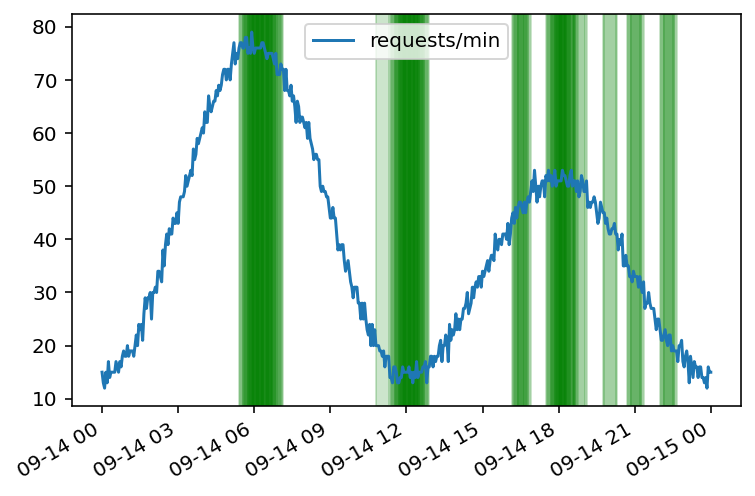
\includegraphics[width=4in]{img/stable_workload_threshold_example.png}
		\caption{Example of stable windows detected by Min-Max algorithm using a threshold of 6\%.}
		\label{fig:threshold_selection}
	\end{figure}


	
	\subsection{Workload characterization module}  \label{ssec:workload_characterization_module}
	Workload characterization is used to normalize the outcome of each configuration according to the workload type, which is required by contextual Bayesian optimization (section \ref{ssec:contextual_bayesian_optimization}). We are interested in characterizing the workload without any human intervention: for this reason, the module uses clustering-based methods. \\
	The clustering methods that have been chosen are $k$-means, mean shift, Gaussian Mixture Models (GMM), and OPTICS (see section \ref{ssec:clustering}).
	
	Since $k$-means requires the number of clusters $k$ to be given as input, the quality of clustering is evaluated for each size $k \in K, K = [2, \max (3, \log n)]$ where $n$ is the number of workload points. The evaluation is performed computing the Silhouette score for each $k$, and selecting the value that leads to the highest score:\\\\
	\centerline{
	$
		k = \underset{k \in K}{\mathrm{argmax}}\, S(W, l_k)
	$
	}\\\\
	where $S$ is the Silhouette score, $W$ is the set of workload points, and $l_k$ are the labels obtained by applying $k$-means to find $k$ clusters.
	
	Mean shift doesn't require to set the number of clusters beforehand, but it must be provided with the size of the bandwidth used in the RBF kernel. The bandwidth is estimated using $k$-nearest neighbor on a down-sampled workload dataset to reduce the computation time.
	
	GMM must be provided with the number of components (i.e. clusters) to look for and the covariance type. These parameters are chosen by maximizing the Bayesian Information Criterion (BIC):\\\\
	\centerline{
		$
		(n, cv) = \underset{n \in N, cv \in CV}{\mathrm{argmax}}\, BIC(C_{n, cv})
		$
	}\\\\
	where $n$ is the number of components, $cv$ is the covariance type, and $C_{n, cv}$ is the clustering obtained using GMM with $n$ and $cv$. Similarly to $k$-means the range of the number of clusters to find is $N = [2, \max (3, \log n)]$. $CV$ is the set of available covariance types, e.g \textit{spherical}, and \textit{diagonal}.
	
	Finally, OPTICS clustering is performed using the Euclidean distance and with different values of $\xi$, that controls a cluster boundary. Similarly to $k$-means, the best value of $\xi$ is chosen by maximizing the Silhouette score: \\\\
	\centerline{
		$
		\xi = \underset{\xi \in \Xi}{\mathrm{argmax}}\, S(W, l_\xi)
		$
	}\\\\
	where $\Xi$ is the set of possible $\xi$ values, and $l_\xi$ are the labels obtained by applying OPTICS on the workload dataset $W$ using $\xi$. The workload points marked as outliers are assigned to a dedicated cluster containing just one point.
	
	In all cases, since the properties composing the workload may have different scales (e.g. number of users and read/write ratio), they are all scaled in the $[0, 1]$ range using a min-max scaler.	Furthermore, with all methods except OPTICS, the size of the input dataset $W$ is limited by randomly sampling $N$ points from $W$ so that the computation effort required by the clustering methods is limited.	
	
	Finally, the dataset $W$ is initialized together with the forecasting module: the workload points seen during the initialization period (e.g. the first week) are included so that the tuner is provided with meaningful workload groups since the beginning of the optimization process.

	\section{Experimental setup } \label{sec:exp_setup}
	The proposed solution has the goal of extending the existing tuner \cite{AkamasCGP} to work in an online manner. Therefore, we are interested in how quickly we are able to find a good configuration while avoiding bad ones. Nevertheless, the effectiveness of the tuning depends on two key factors: the ability of selecting as many stable workload windows as possible, that increases the number of experiments and therefore how quickly we can optimize the objective function, while avoiding unstable workload windows that are likely to lead to failures or low QoS levels. This selection ability,  along with the quality of the configuration proposed by the tuner, strongly depends on the forecasting accuracy.\\
	Therefore, we evaluate the forecasting module and the window selection algorithm independently from the tuner (section \ref{ssec:exp_workload_forecasting} and \ref{ssec:exp_stable_wkld_finder}). The workload characterization module, that is based on clustering algorithms, is evaluated qualitatively. The overall solution is evaluated by using DBMS models (section \ref{ssec:exp_online_cgp}) that map the configuration space to a wide variety of performance metrics (according to the perceived workload), allowing us to run reproducible tests on a local machine.
	
	To evaluate each component we chose a set of four time series to make the experiments reproducible (figure \ref{fig:time_series}). Such time series represent the number of users connected to the system being optimized, i.e. the DBMS models.  Two time series are synthetically generated by creating a daily and a weekly pattern. The daily pattern time series has three variants with increasing noise to make a sensibility analysis (figure \ref{fig:daily_noises}). The remaining two time series are obtained from real data: the number of taxi requests in the city of New York and the number of requests to a bank system. Note that all time series have been mapped to the $[10, 80]$ range to be compatible with the DBMS models. \\
	Furthermore, besides the number of requests, the workload can be affected by a benchmark that represents the behavior of the users at a certain time (e.g. are the users just reading data from the DBMS or are they inserting data?). We model this property of the workload by using three types of user behavior: read-intensive, write-intensive, and balanced.
	\begin{figure}\centering
		\subfloat[Daily pattern]{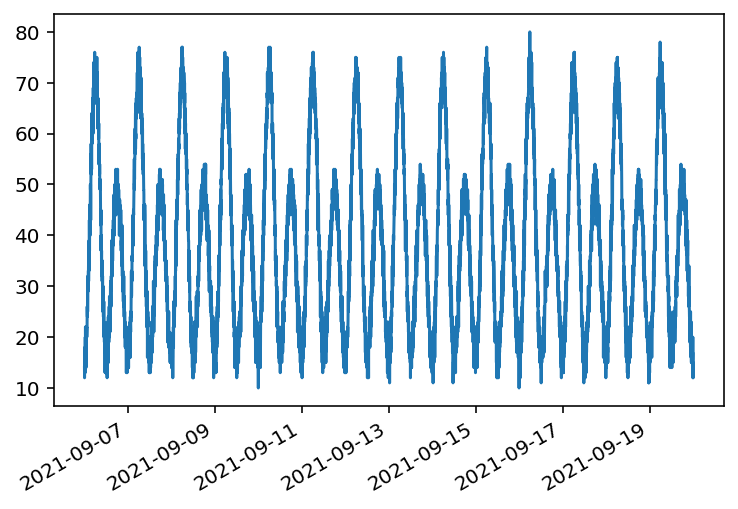
\includegraphics[width = 2in]{img/ts/daily.png}} 
		\subfloat[Weekly pattern]{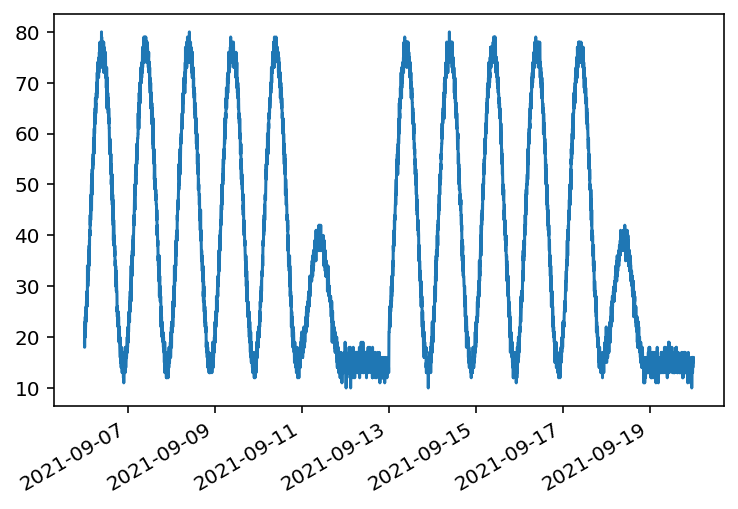
\includegraphics[width = 2in]{img/ts/weekly.png}} \hfill
		\subfloat[Taxi requests]{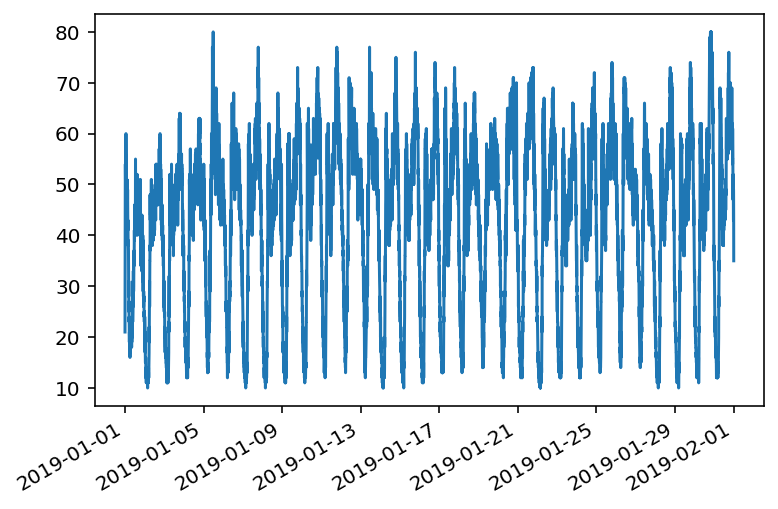
\includegraphics[width = 2in]{img/ts/taxi.png}} 
		\subfloat[Bank requests]{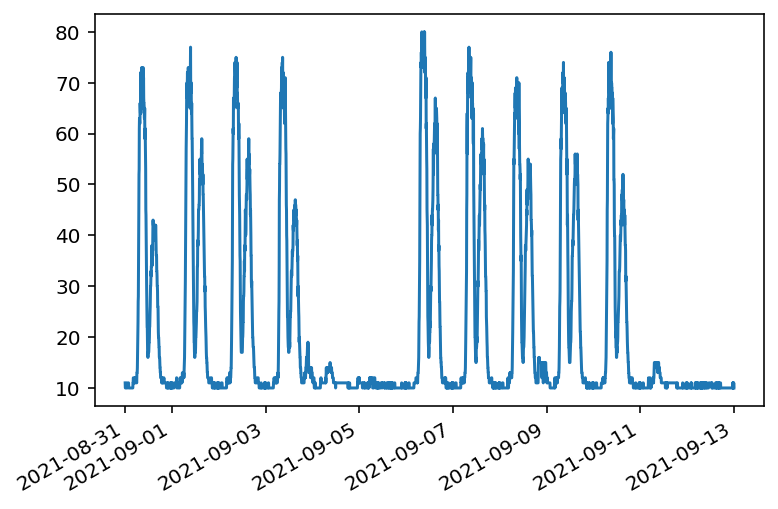
\includegraphics[width = 2in]{img/ts/bank.png}} 
		
		\caption{Workload time series.}
		\label{fig:time_series}
	\end{figure}
	
	\begin{figure}\centering
		\subfloat[Daily 0.02 stddev noise]{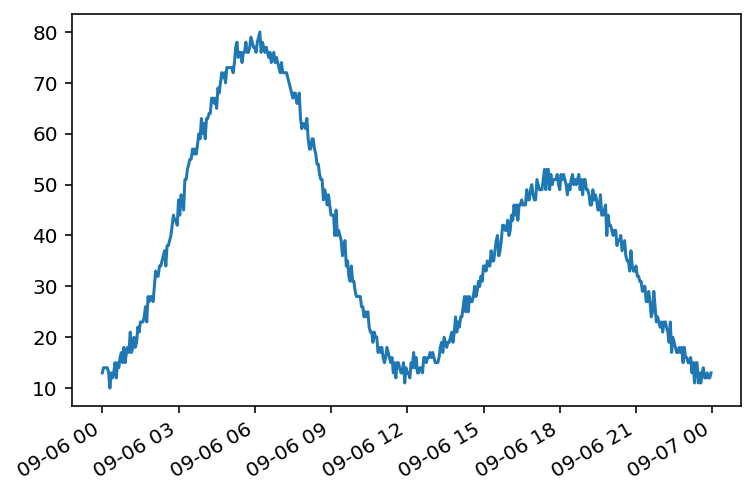
\includegraphics[width = 2in]{img/ts/daily_zoom_02.png}} 
		\subfloat[Daily 0.04 stddev noise]{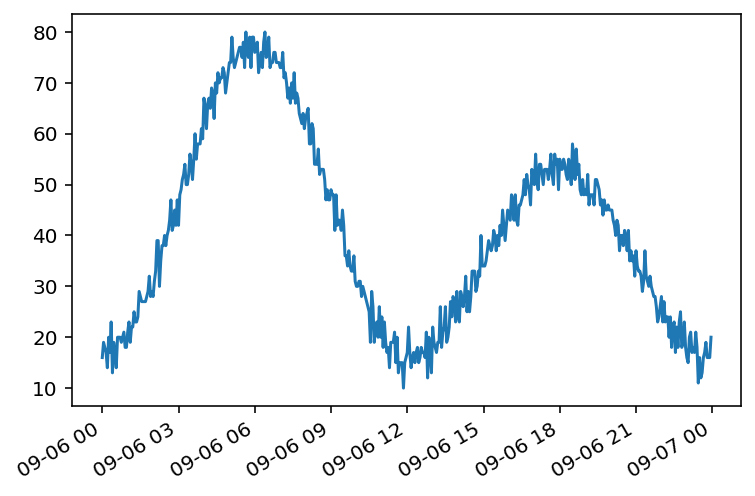
\includegraphics[width = 2in]{img/ts/daily_zoom_04.png}} \hfill
		\subfloat[Daily 0.08 stddev noise]{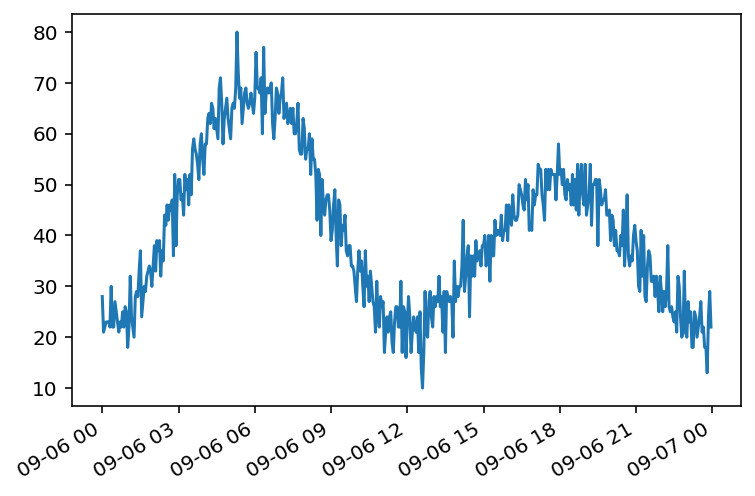
\includegraphics[width = 2in]{img/ts/daily_zoom_08.png}} 
		
		\caption{Zoomed daily pattern with increasing noise.}
		\label{fig:daily_noises}
	\end{figure}
	
	Finally, we are interested in the performance of the developed solution when the amount of time series data provided to the forecaster covers less than one week. By exploring such case when using time series with weekly seasonality we can also understand how the system reacts to patterns that are not present in the historical data (e.g. the reduced number of requests during the weekend when the forecaster has only four days of historical data).
	
	\subsection{Workload Forecasting } \label{ssec:exp_workload_forecasting}
	To evaluate the forecasting accuracy we chose two metrics: the Mean Absolute Percentage Error (MAPE) and the Root Mean Squared Error (RMSE).  Remembering that we are repeatedly forecasting short-term windows while new workload data is incoming, we are interested in the overall errors up to the latest measurement plus how wrong the forecaster is in a specific moment.
	
	Formally, when evaluating the accuracy of a time series starting at time $t_0$ and we have data up to time $t_1$, for each forecasted window $\omega_{t:t+\delta}$ where $\delta$ is the length of the short term forecast, we compute the error of the associated forecast $\tilde{\pmb{y}}_{t:t+\delta}$ using the true values $\pmb{y}_{t:t+\delta}$, for $t=t_0, ..., t_1 - \delta$. Then, we merge the forecasts and compute the error up to time $t_1 - \delta$. As we receive new time series data over time (i.e. $t_1$ increases over time), the latter is called incremental MAPE or RMSE. \\
	Figure \ref{fig:exp_setup_forecasting} shows a time series with naive forecasts, the per-forecast error and the incremental error evolving over time when the tuning windows have length $1$ hour.
	
	The error of a forecasting model in a specific moment can be used to inspect the performance of a single model, eventually automatically triggering a re-fitting process when the error exceeds a threshold. For example, picture $(b)$ in figure \ref{fig:exp_setup_forecasting} clearly shows a huge forecasting error on date 2019-01-28 given by configuration zero. On the other side, the incremental error can be used to compare different forecasting models and how the errors change after a model has been re-fitted (e.g. new data has been included). The latest value of the incremental error is of particular interest, as it represents the up-to-date overall performance of a model.
	
	\begin{figure}\centering
		\subfloat[Naive forecasts (red) based on previous day value.]{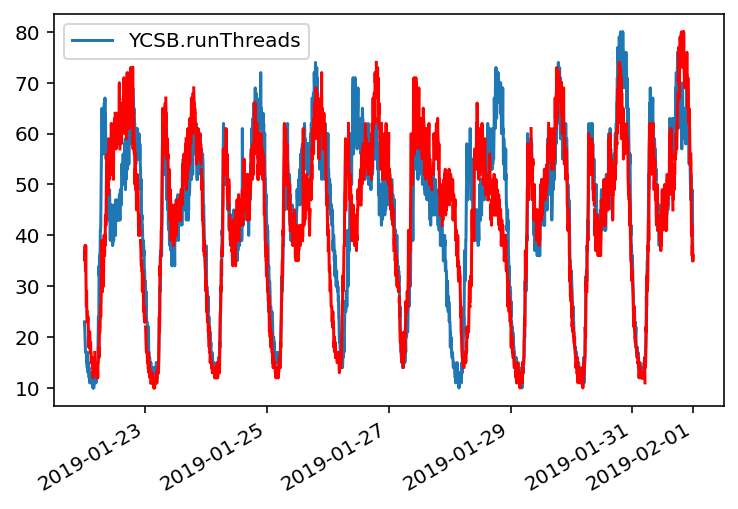
\includegraphics[width = 3in]{img/exp_setup_example_forecasts.png}} \hfill
		\subfloat[Per-forecast MAPE.]{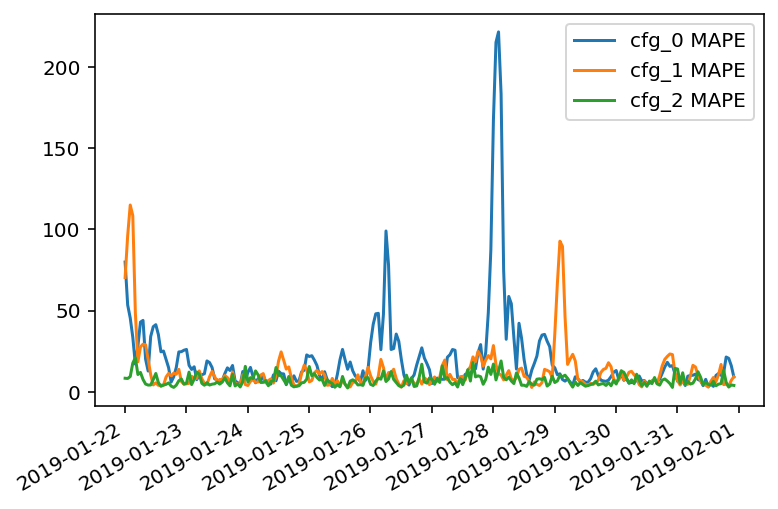
\includegraphics[width = 3in]{img/exp_setup_per_forecast_mape.png}} \hfill
		\subfloat[Incremental MAPE.]{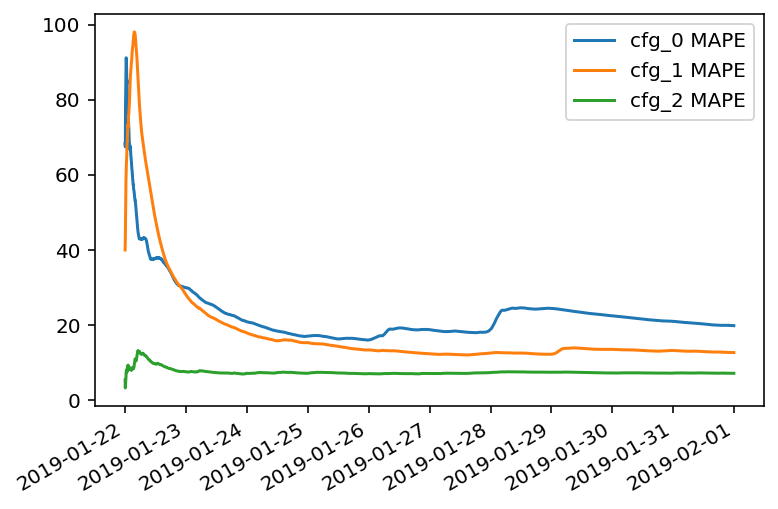
\includegraphics[width = 3in]{img/exp_setup_incremental_mape.png}} 
		
		\caption{Per-forecast and incremental MAPE example of three models. The forecast shown in picture $(a)$ is given by configuration $0$.}
		\label{fig:exp_setup_forecasting}
	\end{figure}
	
	The MAPE has the following formula:\\\\
	\centerline{
	$
	\text{MAPE}(\pmb{y}_{t:t+m}, \tilde{\pmb{y}}_{t:t+m}) = \frac{100}{m} \sum_{i=t}^{t+m} |\frac{\pmb{y}_{t:t+m}-\tilde{\pmb{y}}_{t:t+m}}{\pmb{y}_{t:t+m}}|
	$
	}\\\\
	and the RMSE:\\\\
	\centerline{
		$
		\text{RMSE}(\pmb{y}_{t:t+m}, \tilde{\pmb{y}}_{t:t+m}) = \sqrt{\frac{\sum_{i=t}^{t+m} (y_i - \tilde{y}_i)^2 }{m}}
		$
	}\\\\
	
	The two metrics may look redundant, but since the RMSE gives more importance to the highest errors, by considering the RMSE over the MAPE we are actually increasing sensitivity to outliers. Furthermore, using RMSE we seek to be correct on average, while in contrast the MAPE targets the median.\\
	Finally, note that the MAPE is easier to understand as it express the error as a percentage that is independent from the scale of the time series. Therefore, it is useful to compare the performance of a model on different time series. Nevertheless, MAPE cannot be used when the values are too close to zero.
	
	\subsection{Stable workload finder } \label{ssec:exp_stable_wkld_finder}
	The stable workload finder algorithm uses the forecast of the upcoming workload and its historical data to predict if a time window in the upcoming future will be stable or not. Therefore, it acts as a binary classifier that should detect a decent amount of stable windows while avoiding unstable ones. As mentioned in section \ref{ssec:stable_window_finder}, we give more importance to avoiding false positives (see table \ref{table:stability_cases}) as they facilitate failures.
	
	To evaluate such classifier, we consider its precision and recall. Precision is defined as:\\\\
	\centerline{
	$
	\text{Precision} = \frac{ True \, Positive}{ True \, Positive + False \, Positive}
	$
	}\\\\
	and Recall as:\\\\
	\centerline{
		$
		\text{Recall} = \frac{ True \, Positive}{ True \, Positive + False \, Negative}
		$
	}\\\\
	Simply put, Precision measures how many of the windows that were marked stable were actually stable, while Recall measures how many (true) stable windows were found by the algorithm. Therefore, we give more importance to the Precision score as it measures how many potentially dangerous experiments the tuner performed. On the other side, a good Recall value means that the tuner exploited as many windows as possible eventually leading to faster optimal convergence, but this shouldn't come at the cost of QoS.
	
	To balance Recall and Precision we use the F1 score:\\\\
	\centerline{
		$
		\text{F1} = 2 \times \frac{ \text{Precision } \times \text{ Recall}}{\text{Precision } + \text{ Recall}}
		$
	}\\\\
	
	\subsection{Online Contextual Gaussian Process Tuner } \label{ssec:exp_online_cgp}
	As mentioned before, the proposed solution is evaluated using DBMS models, namely MongoDB and Cassandra. The models are trained such that they can map the configuration space, specific to each DBMS, to a wide variety of performance metrics \cite{AkamasCGP}, such as throughput and memory usage. By doing so, the experiments are easily reproducible.\\	
	Furthermore, by using database models we know the optimal configuration and we can see how far the tuner is from the real optimum. To do so, we compute the Normalized Performance Improvement at iteration $i$:\\\\
	\centerline{
	$
	NPI(i) = \frac{y_0 - y_i}{y_0 - y^\star} = \frac{f(\pmb{x}_0 \pmb{w}_i) - f(\pmb{x}_i, \pmb{w}_i)}{f(\pmb{x}_0 \pmb{w}_i) - f(\pmb{x}_{\pmb{w}_i}^\star, \pmb{w}_i)}
	$
	}\\\\
	where $\pmb{x}_0$ is the vendor (or baseline) configuration, $\pmb{x}_i$ is the configuration being evaluated at iteration $i$, and $\pmb{x}_{\pmb{w}_i}^\star$ is the optimal configuration for the workload observed at iteration $i$. Therefore, an NPI of zero means that we have the same performance of the vendor configuration, and an NPI of one means that we found the global optimum. 
	
	To evaluate the entire tuning process up to iteration $i$ we use the Cumulative Reward (CR):\\\\
	\centerline{
		$
		CR(i) = \sum_{j=0}^{i} NPI(j)
		$
	}\\\\
	that has a constant unitary slope if the tuner is optimal, is equal to zero if the baseline is repeatedly applied, and has no lower bounds for bad configurations.\\
	By using normalized performance metrics we can quantitatively compare and evaluate tuners independently from the workload, taking into consideration the number of iterations required by the tuner to find a good configuration.
	
	Furthermore, we consider the cumulative number of failures occurred up to iteration $i$:\\\\
	\centerline{
		$
		\text{Failures(i)} = \sum_{j=0}^{i} F(j)
		$
	}\\\\
	where $F(j)$ is one if a failure occurred at iteration $j$, zero otherwise. The constraint we are imposing to the tuners are to keep the latency (i.e. the response time) below some QoS target when tuning the MongoDB model, and keep the memory requirements below a specific level when tuning the Cassandra model.\\
	The objective functions being minimized are the memory requirements for MongoDB and the latency for Cassandra.
	
	Finally, when evaluating tuners, we are interested in how many iterations are required to outperform the baseline tuner in terms of CR. We expect that at the beginning of the tuning process the tuner needs to explore the configuration space, suggesting configurations that are worse than the baseline. After a few iterations, the suggested configurations will be better than the baseline (i.e. the configurations will have a score higher than 0) so that the CR of the tuner will eventually overtake the CR of the Baseline tuner. We name this metric Time To Recover (TTR).
	
	\section{Results } \label{sec:results}
	This section presents the results according to the setup presented in section \ref{sec:exp_setup}. Workload characterization is evaluated qualitatively. 
	
	\subsection{Workload Characterization } \label{ssec:results_wkld_characterization}
	The workload characterization, performed with clustering methods, is evaluated qualitatively.
	By doing so, we must remember that each workload type (i.e. cluster) will group the points that will be used by the tuner to normalize the score. Therefore, it is important for each cluster to contain a meaningful amount of points so that the tuner can understand which configurations are better/worse under a given workload type. For this reason, OPTICS turned out to be unusable due to the high number of identified clusters (often above 1000), where a significant amount of clusters were made of just one point. Note that such issue could be solved by changing the parameters according to the dataset being clustered, at the cost of losing the autonomy of the workload characterization module.  
	
	By using Gaussian Mixture Models, a probabilistic approach that uses different covariance types, the number of identified clusters on a given dataset is inconsistent: running the algorithm multiple times returns a clustering with different covariance types and number of components (chosen by maximizing the BIC). This outcome is even accentuated after down-sampling the dataset, which is required to limit the amount of time required to find the clusters. Furthermore, GMM is prone to assign different clusters to points that are expected to belong to the same cluster. This behavior is shown in figure \ref{fig:results_gmm}, where low-demand zones are assigned to different workload types.
	
	\begin{figure}
		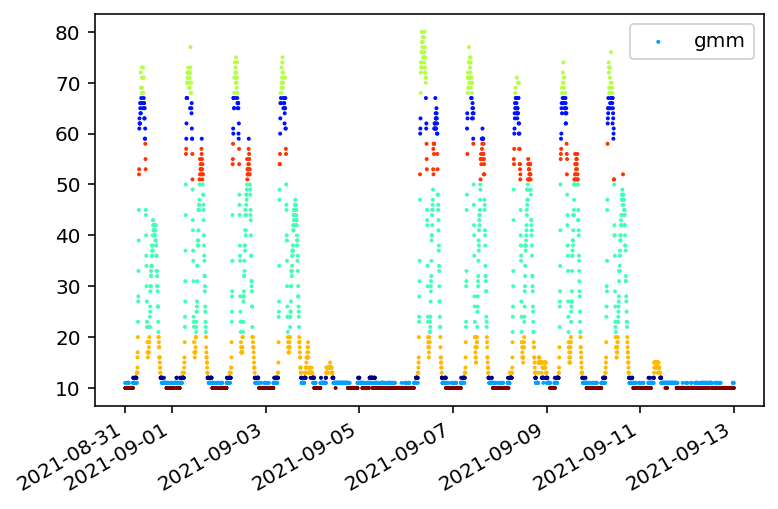
\includegraphics[width=4in]{img/results_clustering_gmm.png}
		\caption{GMM clustering on time series $(d)$ (bank requests). Each color is a cluster (there are a total of 8 clusters). The low-demand zone is clearly over-separated.}
		\label{fig:results_gmm}
	\end{figure}

	By excluding OPTICS and GMM we are left with $k$-means and mean shift. As expected, $k$-means returns spherical-shaped clusters so that the associated workload types are well-separated. This behavior is shown in figure \ref{fig:results_clustering_kmeans}. The clustering obtained with mean shift is shown in picture \ref{fig:results_clustering_meanshift}.
	
	\begin{figure}\centering
		\subfloat[Daily pattern]{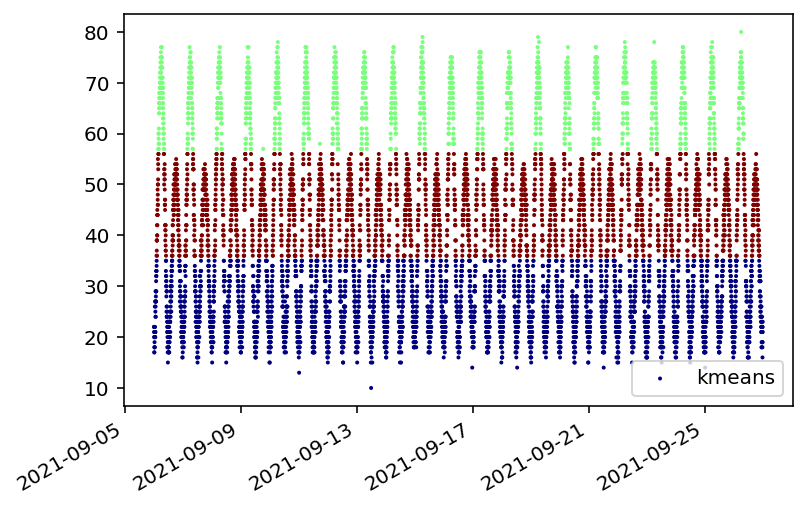
\includegraphics[width = 2.5in]{img/results_clustering_kmeans_daily.png}} 
		\subfloat[Weekly pattern]{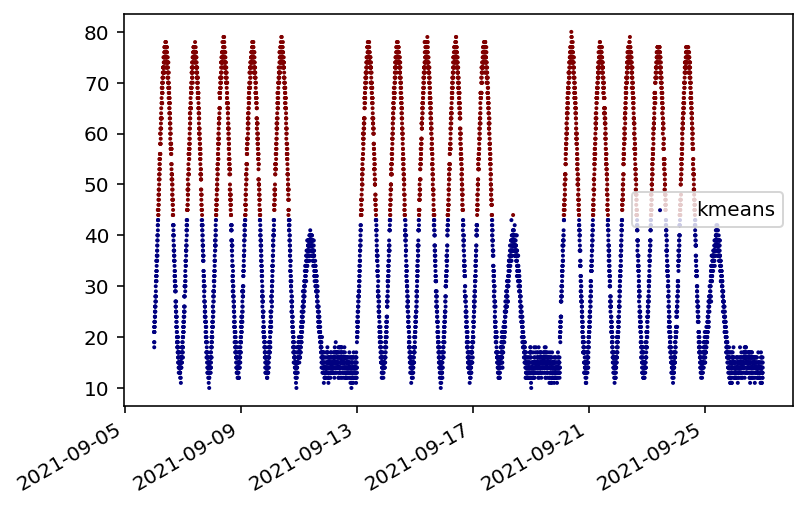
\includegraphics[width = 2.5in]{img/results_clustering_kmeans_weekly.png}} \hfill
		\subfloat[Taxi requests]{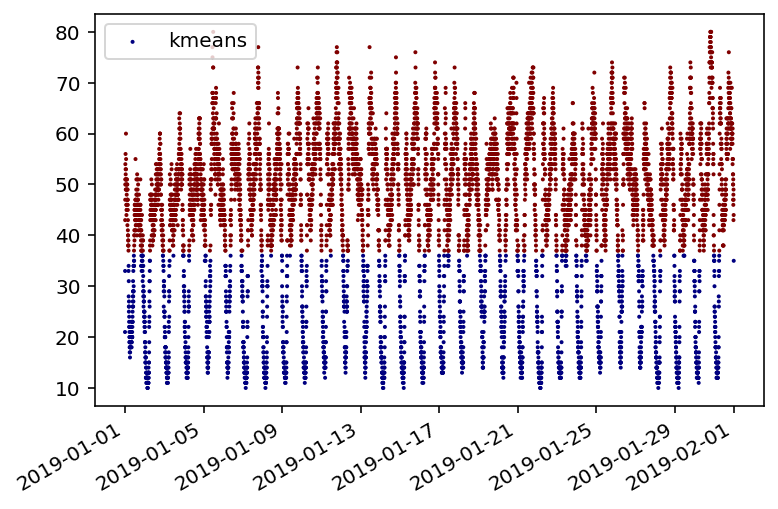
\includegraphics[width = 2.5in]{img/results_clustering_kmeans_taxi.png}} 
		\subfloat[Bank requests]{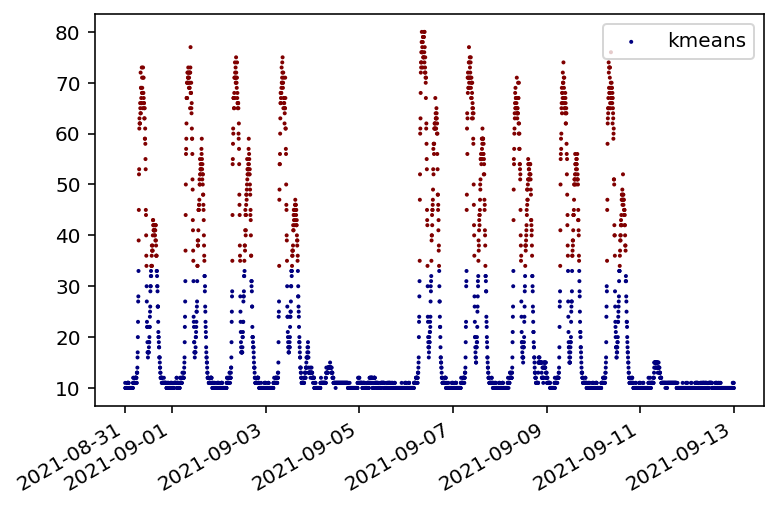
\includegraphics[width = 2.5in]{img/results_clustering_kmeans_bank.png}} 
		
		\caption{Results of clustering the workload using $k$-means. Points with the same color belong to the same cluster.}
		\label{fig:results_clustering_kmeans}
	\end{figure}
	
	\begin{figure}\centering
		\subfloat[Daily pattern]{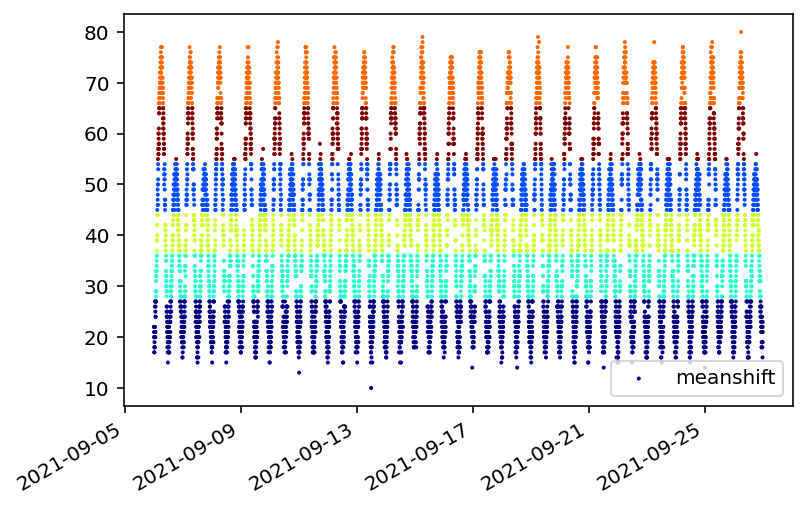
\includegraphics[width = 2.5in]{img/results_clustering_meanshift_daily.png}} 
		\subfloat[Weekly pattern]{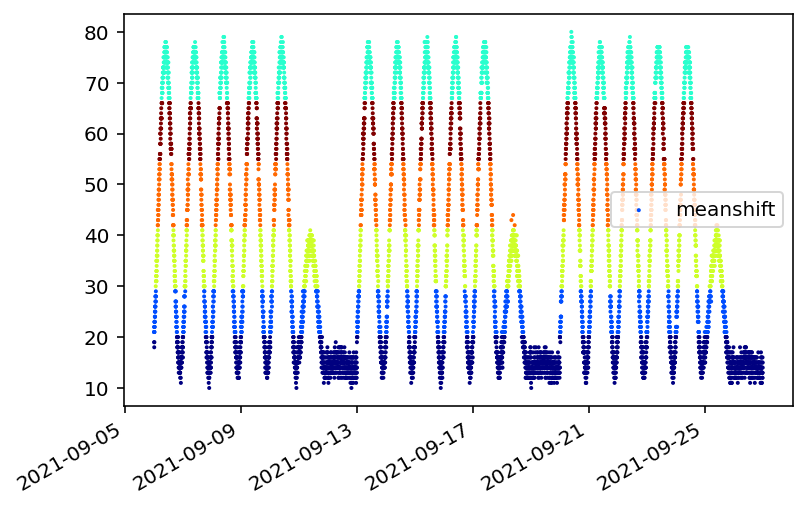
\includegraphics[width = 2.5in]{img/results_clustering_meanshift_weekly.png}} \hfill
		\subfloat[Taxi requests]{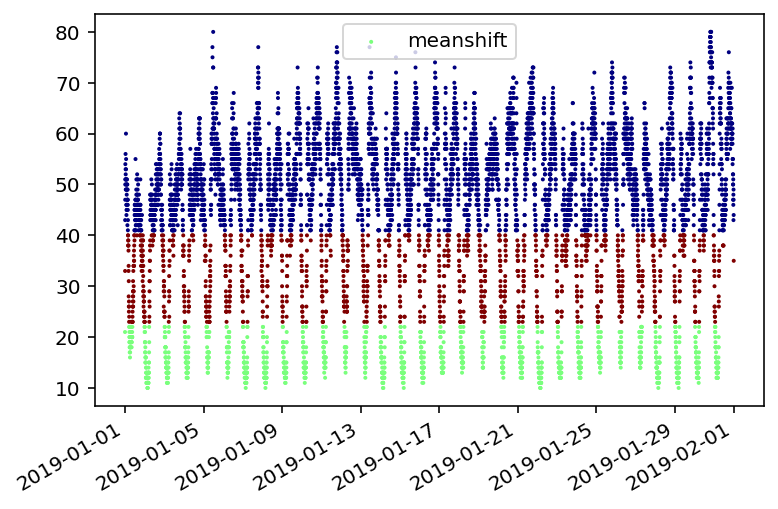
\includegraphics[width = 2.5in]{img/results_clustering_meanshift_taxi.png}} 
		\subfloat[Bank requests]{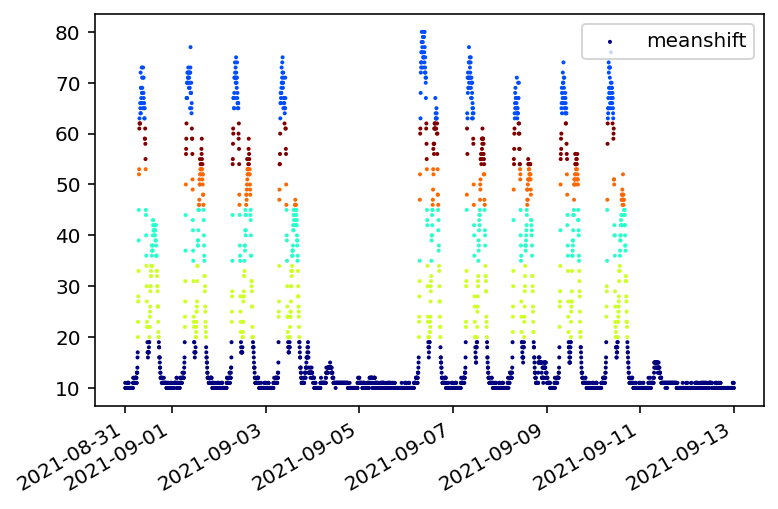
\includegraphics[width = 2.5in]{img/results_clustering_meanshift_bank.png}} 
		
		\caption{Results of clustering the workload using mean shift. Points with the same color belong to the same cluster.}
		\label{fig:results_clustering_meanshift}
	\end{figure}

	Comparing $k$-means with mean shift, it is clear that mean shift generally finds more clusters. The impact of such difference depends on how the tuner is able to exploit the collected knowledge, and is therefore further discussed later.  Nevertheless, finding more workload types requires more time to populate each cluster with tuning experiments. Therefore, the clustering method should be chosen specifically for each workload pattern. Note that such choice can be made at any step of the tuning process: we may start with $k$-means and then switch to mean shift once there is enough data.
	
	\clearpage
	\subsection{Forecasting} \label{ssec:results_forecasting}
	This section is organized as follow: for each time series in figure \ref{fig:time_series} we show the per-forecast errors and the incremental errors (see section \ref{ssec:exp_workload_forecasting}). 
	The synthetic time series (daily and weekly pattern) have their per-forecast error computed on forecasts of length 1 hour, performed every 30 minutes, while the real-world time series models make forecasts of length 45 minutes every 15 minutes. The reason for such difference is that the volatility of the latter time series is much higher, with tops that are reached in less than thirty minutes. By re-computing forecasts every 15 minutes, deep learning models are allowed to exploit the latest data and quickly react to ramps.
	
	All models presented in section \ref{ssec:workload_forecasting} are compared using the following names:
	\begin{itemize}
		\item \textit{cfg\_0}: naive model used as baseline that makes predictions using previous day or week data.
		\item \textit{cfg\_1}: Prophet model.
		\item \textit{cfg\_2}: DeepAR model.
		\item \textit{cfg\_3}: MQCNN model.
		\item \textit{cfg\_4}: DeepState model.
	\end{itemize}
	
	\subsubsection{Daily time series} \label{sssec:results_forecasting_daily}
	The daily time series models are trained with 7 days of historical data, independently from the noise level. Once more data is available, the models are not retrained: they are expected to extract the pattern within the data collection period.  The results on the daily pattern with $0.02$ standard deviation noise are shown in figure \ref{fig:results_forecasting_daily_02}, while the results for all the time series variants with increasing noise are summarized in table \ref{table:results_forecasting_daily_patterns}, which shows the final MAPE and RMSE.\\ 
	Prophet and DeepAR are the models that achieve the best performance considering the increasing noise, with DeepAR being the most resilient to noise. Interestingly, when qualitatively evaluating the forecasts of DeepAR and MQCNN on the lowest noise variant, DeepAR looks preferable due to forecasts that better match the underlying daily pattern, as shown in picture \ref{fig:results_forecasting_daily_02_mqcnn_deepar}. 
	
	\begin{figure}\centering
		\subfloat[Per-forecast MAPE]{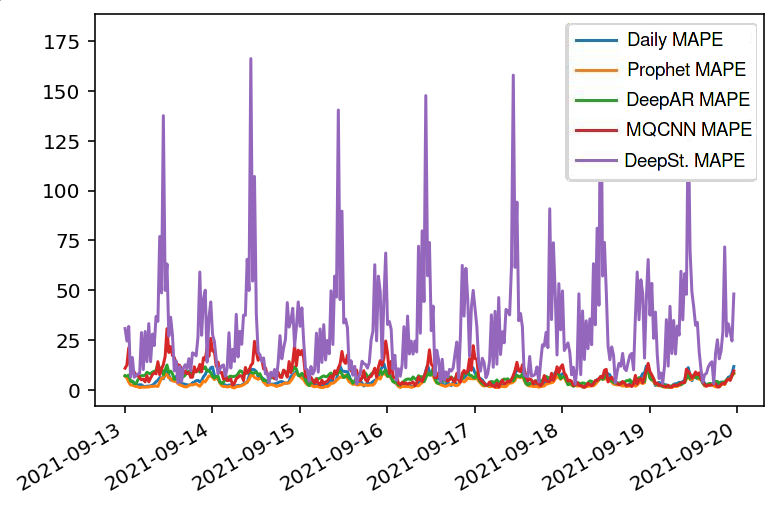
\includegraphics[width = 2.5in]{img/results_forecasting_daily_02_fc_mape.png}} 
		\subfloat[Per-forecast RMSE]{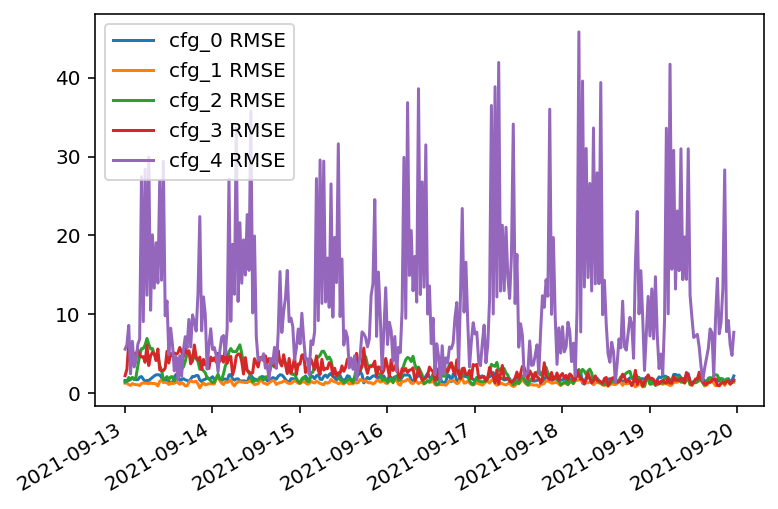
\includegraphics[width = 2.5in]{img/results_forecasting_daily_02_fc_rmse.png}} \hfill
		\subfloat[Incremental MAPE]{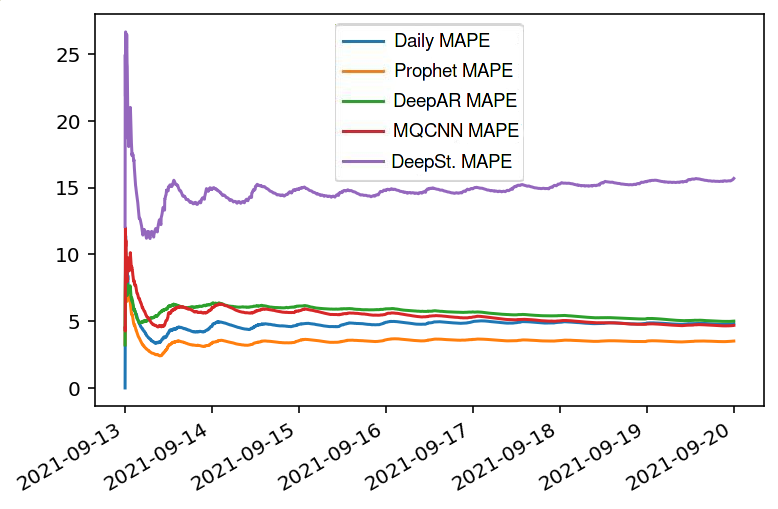
\includegraphics[width = 2.5in]{img/results_forecasting_daily_02_incr_mape.png}} 
		\subfloat[Incremental RMSE]{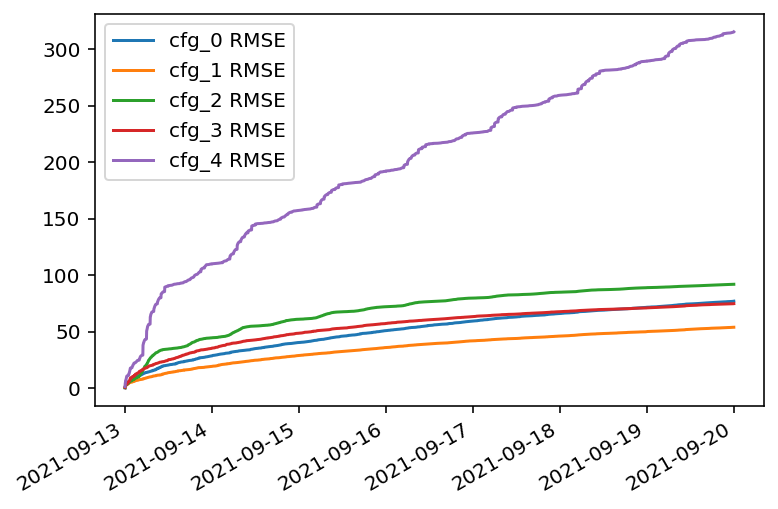
\includegraphics[width = 2.5in]{img/results_forecasting_daily_02_incr_rmse.png}} 
		
		\caption{Errors on daily pattern time series, with 0.02 std dev. noise.}
		\label{fig:results_forecasting_daily_02}
	\end{figure}

	\begin{table*}\centering 
		\ra{1.3}
		\begin{tabular}{@{}rcrc@{}}
			\cmidrule(l){1-4} %\toprule
			& Model & MAPE & RMSE\\
			\cmidrule(l){1-4} 
			\multirow{5}{*}{0.02 std dev. noise}
			& Daily & 4.81 & 76.85\\
			&Prophet & 3.51 & 53.76\\
			&DeepAR & 5.0 & 91.82\\
			&MQCNN & 4.67 & 74.67\\
			&DeepState & 15.68 & 315.33\\
			
			\cmidrule(l){1-4} 
			\multirow{5}{*}{0.04 std dev. noise}
			& Daily & 7.23 & 127.10\\
			&Prophet & 5.22 & 90.40\\
			&DeepAR & 7.25 & 138.40\\
			&MQCNN & 9.92 & 183.99\\
			&DeepState & 12.70 & 270.68\\
			
			\cmidrule(l){1-4} 
			\multirow{5}{*}{0.08 std dev. noise}
			& Daily & 11.67 & 213.15\\
			&Prophet & 8.51 & 154.55\\
			&DeepAR & 8.87 & 165.33\\
			&MQCNN & 10.86 & 212.58\\
			&DeepState & 52.76 & 1841.80\\
			\bottomrule
		\end{tabular}
		\caption{Results on daily patterns with increasing noise. The daily model produces forecasts repeating data of the previous day.} \label{table:results_forecasting_daily_patterns}
	\end{table*}
	
	\begin{figure}\centering
		\subfloat[DeepAR forecasts]{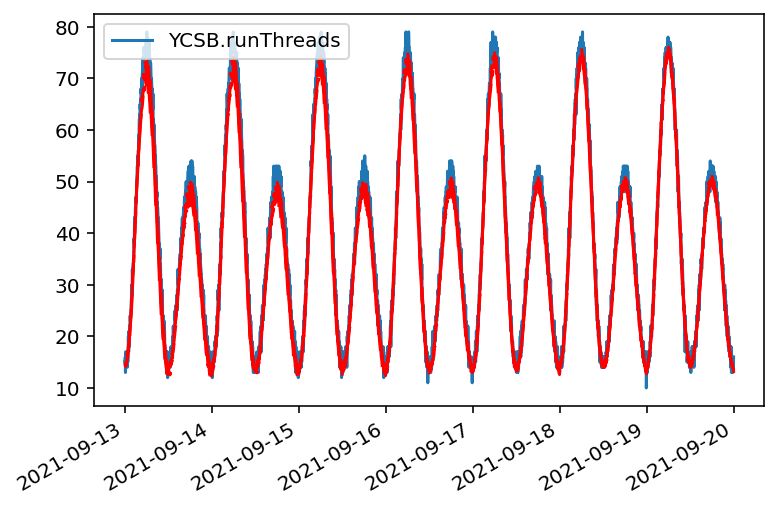
\includegraphics[width = 2.5in]{img/results_forecasting_daily_02_deepar.png}} 
		\subfloat[MQCNN forecasts]{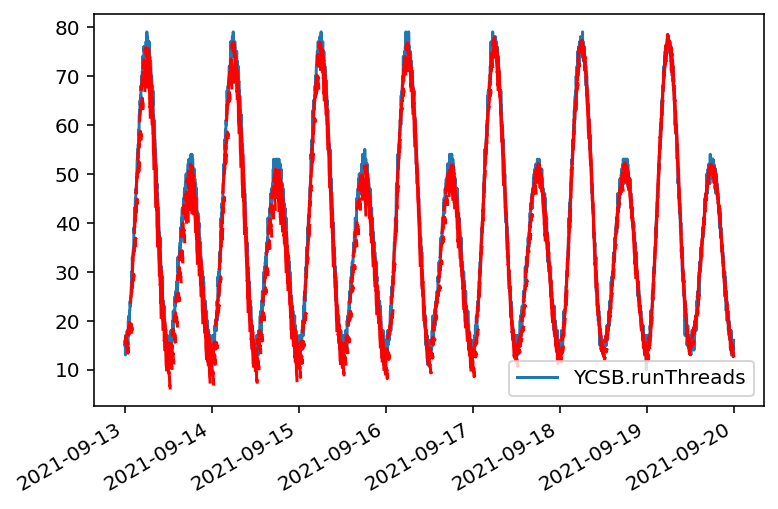
\includegraphics[width = 2.5in]{img/results_forecasting_daily_02_mqcnn.png}} \hfill
		
		\caption{Qualitative comparison of DeepAR and MQCNN on daily pattern with 0.02 std dev. noise. The blue time series is the ground truth.}
		\label{fig:results_forecasting_daily_02_mqcnn_deepar}
	\end{figure}
	
	\clearpage
	\subsubsection{Weekly time series} \label{sssec:results_forecasting_weekly}
	The weekly time series models are trained with 14 days of historical data. The goal of such time series is to understand the ability of a model to extract a weekly pattern.
	 The results are shown in picture \ref{fig:results_forecasting_weekly} and summarized in table \ref{table:results_forecasting_weekly}: the clear winners are Prophet and DeepAR. MQCNN is able to extract the pattern, but fails at predicting the time series' tops, accumulating errors during workdays as shown in figure \ref{fig:results_forecasting_weekly_mqcnn}.
	
	\begin{figure}\centering
		\subfloat[Per-forecast MAPE]{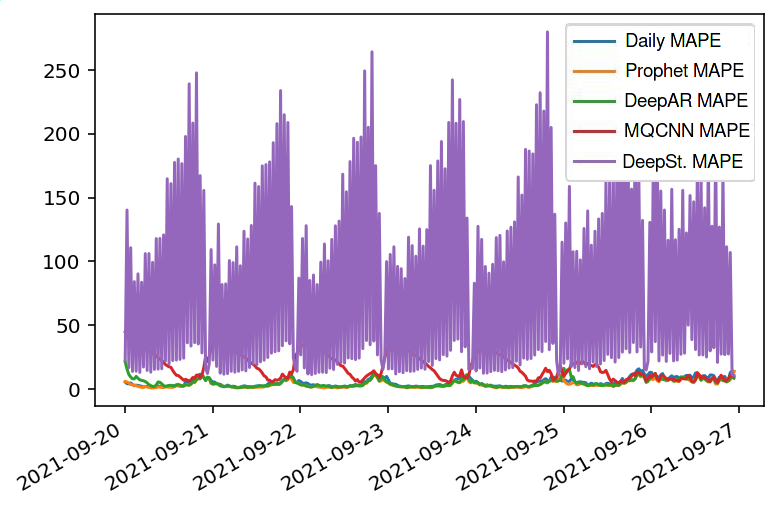
\includegraphics[width = 2.5in]{img/results_forecasting_weekly_fc_mape.png}} 
		\subfloat[Per-forecast RMSE]{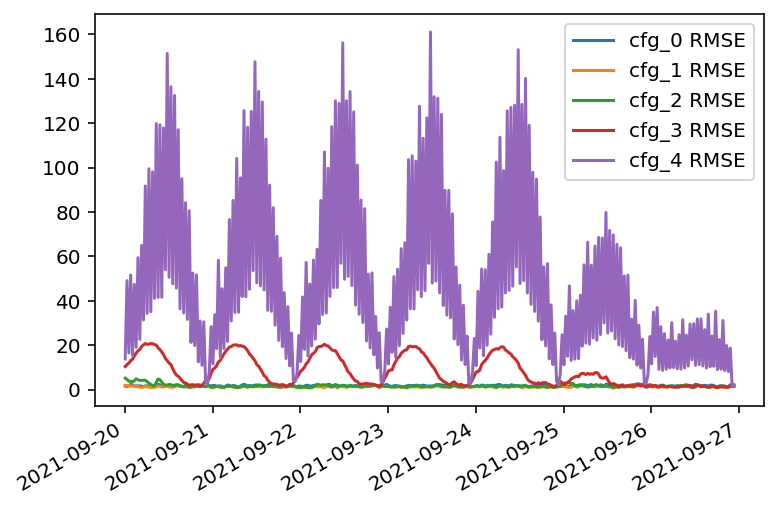
\includegraphics[width = 2.5in]{img/results_forecasting_weekly_fc_rmse.png}} \hfill
		\subfloat[Incremental MAPE]{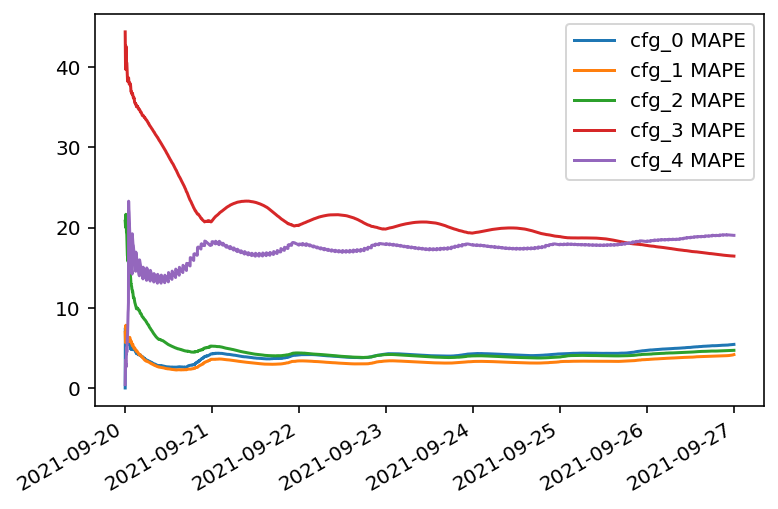
\includegraphics[width = 2.5in]{img/results_forecasting_weekly_incr_mape.png}} 
		\subfloat[Incremental RMSE]{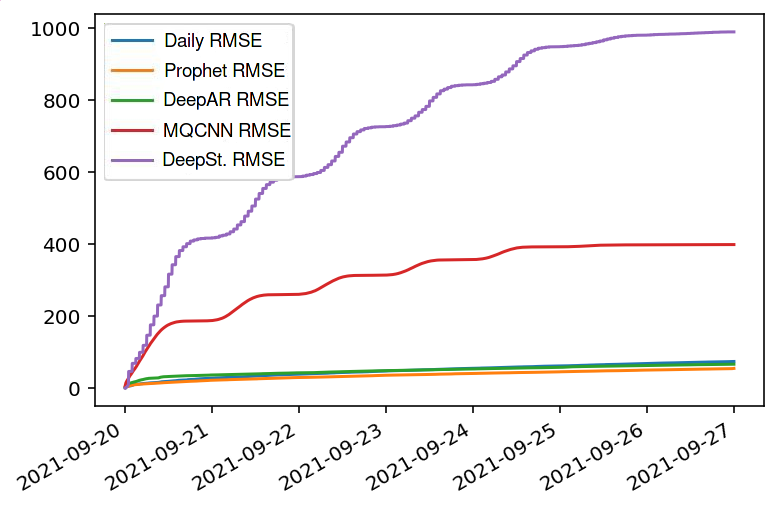
\includegraphics[width = 2.5in]{img/results_forecasting_weekly_incr_rmse.png}} 
		
		\caption{Errors on weekly pattern time series.}
		\label{fig:results_forecasting_weekly}
	\end{figure}
	
	\begin{table*}\centering 
		\ra{1.3}
		\begin{tabular}{@{}crcrc@{}}
			\midrule
			& MAPE & RMSE\\
			\midrule
			Weekly & 5.433 & 73.52\\
			Prophet & 4.16 & 54.32\\
			DeepAR & 4.69 & 65.93\\
			MQCNN & 16.44 & 398.02\\
			DeepState & 19.03 & 988.35\\
			\bottomrule
		\end{tabular}
		\caption{Results on weekly pattern with increasing noise. The Weekly model produces forecasts repeating data of the previous week.} \label{table:results_forecasting_weekly}
	\end{table*}

	\begin{figure} \centering
		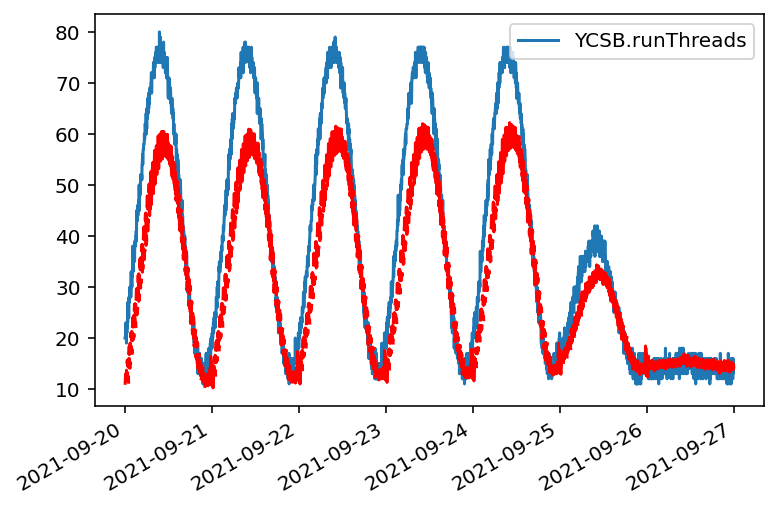
\includegraphics[width=4in]{img/results_forecasting_weekly_mqcnn.png}
		\caption{Forecasting of MQCNN model on weekly time series. The ground truth is blue.}
		\label{fig:results_forecasting_weekly_mqcnn}
	\end{figure}
	
	\clearpage
	\subsubsection{Bank time series} \label{sssec:results_forecasting_bank}
	The bank time series was obtained from real-world data, and due to its shortness the data collection period was set to one week. To balance such lack of data the models are retrained every day. 
	
	This time series is heavily affected by the working hours: in just thirty minutes after the workday started the number of requests per second raises from bottom to top, requiring the models to be able to quickly react to changes. Results are shown in figure \ref{fig:results_forecasting_bank} and summarized in table \ref{table:results_forecasting_bank}. 
	
	By checking the DeepAR per-forecast error and forecast, we can see that the Saturday ramp causes a fake out where the model predicts a spike similar to the previous working days. This behavior could be caused by a lack of data.
	
	As mentioned before, by reducing the forecast interval the deep learning models are able to react ramp signals quicker. Figure \ref{fig:results_forecasting_bank_deepar} shows the impact of forecasting every 15 and 30 minutes.
	
	The Prophet model achieves a high error when compared to the other models. Nevertheless, its predictions are not too bad: what contributes to the high errors is the weekend, that is not properly modeled. This issue could be solved by further increasing the number of Fourier terms for the weekly seasonality, however by doing so we would risk overfitting.
	
	
	\begin{figure}\centering
		\subfloat[Per-forecast MAPE]{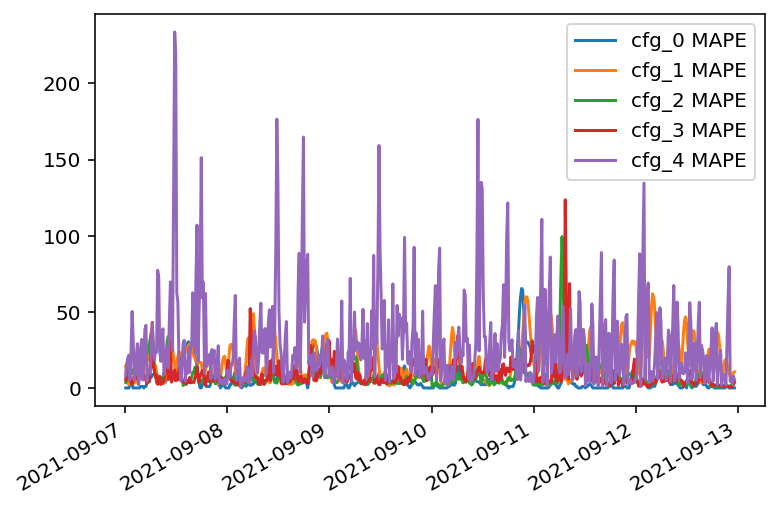
\includegraphics[width = 2.5in]{img/results_forecasting_bank_fc_mape.png}} 
		\subfloat[Per-forecast RMSE]{\includegraphics[width = 2.5in]{img/results_forecasting_bank_fc_rmse.png}} \hfill
		\subfloat[Incremental MAPE]{\includegraphics[width = 2.5in]{img/results_forecasting_bank_incr_mape.png}} 
		\subfloat[Incremental RMSE]{\includegraphics[width = 2.5in]{img/results_forecasting_bank_incr_rmse.png}} 
		
		\caption{Errors on weekly pattern time series.}
		\label{fig:results_forecasting_bank}
	\end{figure}
	
	\begin{table*}\centering 
		\ra{1.3}
		\begin{tabular}{@{}crcrc@{}}
			\midrule
			& MAPE & RMSE\\
			\midrule
			Weekly & 5.74 & 87.29\\
			Prophet & 16.16 & 111.96\\
			DeepAR & 5.62 & 58.91\\
			MQCNN & 6.58 & 60.68\\
			DeepState & 13.84 & 184.68\\
			\bottomrule
		\end{tabular}
		\caption{Results on bank time series. The Weekly model produces forecasts repeating data of the previous week.} \label{table:results_forecasting_bank}
	\end{table*}

	\begin{figure}\centering
		\subfloat[DeepAR with 30 minutes forecasting interval]{\includegraphics[width = 2.5in]{img/results_forecasting_bank_deepar_30.png}} 
		\subfloat[DeepAR with 15 minutes forecasting interval]{\includegraphics[width = 2.5in]{img/results_forecasting_bank_deepar_15.png}}
		\caption{Impact of forecasting every 30 and 15 minutes respectively. The blue-colored time series is the ground truth.}
		\label{fig:results_forecasting_bank_deepar}
	\end{figure}
	
	\begin{figure} \centering
		\includegraphics[width=4in]{img/results_forecasting_bank_prophet.png}
		\caption{Prophet forecasting. The blue-colored time series is the ground truth.}
		\label{fig:results_forecasting_bank_prophet}
	\end{figure}
	
	\clearpage
	\subsubsection{Taxi time series} \label{sssec:results_forecasting_taxi}
	
	The taxi time series is one month long and was used to study how the models evolve when more data is available. To do so, the data collection period lasts seven days as usual, but every new week the models are re-trained. The time series is characterized by a strong daily seasonality with quick rises and drops, therefore the models shouldn't suffer from fake outs like with the bank time series. The results are shown in figure \ref{fig:results_forecasting_taxi} and table \ref{table:results_forecasting_taxi}. 
	
	DeepAR achieve the best results both in terms of MAPE and RMSE, while DeepState had to be excluded from the per-forecast errors as they are too high. Except DeepState, all the models improve as new data becomes available. Prophet errors are heavily affected by a great mistake made at the beginning of the forecasting, recovering gradually. Nevertheless, the taxi time series has peaks that don't follow a strong daily or weekly seasonality, and Prophet often fails to catch the tops and bottoms. Figure \ref{fig:results_forecasting_taxi_prophet_deepar} compares Prophet and DeepAR forecasts.
	
	\begin{figure}\centering
		\subfloat[Per-forecast MAPE]{\includegraphics[width = 2.5in]{img/results_forecasting_taxi_fc_mape.png}} 
		\subfloat[Per-forecast RMSE]{\includegraphics[width = 2.5in]{img/results_forecasting_taxi_fc_rmse.png}} \hfill
		\subfloat[Incremental MAPE]{\includegraphics[width = 2.5in]{img/results_forecasting_taxi_incr_mape.png}} 
		\subfloat[Incremental RMSE]{\includegraphics[width = 2.5in]{img/results_forecasting_taxi_incr_rmse.png}} 
		
		\caption{Errors on taxi time series. DeepState per-forecasts errors are not shown as they are high, hiding the other errors.}
		\label{fig:results_forecasting_taxi}
	\end{figure}
	
	\begin{table*}\centering 
		\ra{1.3}
		\begin{tabular}{@{}crcrc@{}}
			\midrule
			& MAPE & RMSE\\
			\midrule
			Daily & 17.76 & 540\\
			Prophet & 14.75 & 451\\
			DeepAR & 6.87 & 214\\
			MQCNN & 9.22 & 297\\
			DeepState & 16.97 & 1061\\
			\bottomrule
		\end{tabular}
		\caption{Results on taxi time series with increasing noise. The daily model produces forecasts repeating data of the previous day. } \label{table:results_forecasting_taxi}
	\end{table*}

	\begin{figure}\centering
		\subfloat[Prophet forecasts]{\includegraphics[width = 2.5in]{img/results_forecasting_taxi_prophet.png}} 
		\subfloat[DeepAR forecasts]{\includegraphics[width = 2.5in]{img/results_forecasting_taxi_deepar.png}}
		
		\caption{Qualitative comparison of Prophet and DeepAR on taxi time series. Forecasts are shown in red.}
		\label{fig:results_forecasting_taxi_prophet_deepar}
	\end{figure}
	
	\clearpage
	\subsubsection{Forecasting results conclusions}
	The results clearly show that DeepState is outperformed by all the other models, despite multiple configurations were tested.  
	
	The DeepAR configuration is the same for all time series except the daily time series, that is simple and can be modeled with a lighter network architecture. Therefore, except for the daily time series, the DeepAR model unrolls one day of past data to make a one-hour forecast. Interestingly, the best configuration found for DeepAR makes use of the custom lags, that improved the modeling of the weekly seasonality, quick rises, and drops. 
	
	Similarly, the MQCNN configuration uses one day of past data to make one-hour predictions. The network decoder size was increased from 30 to 50. The model is trained to minimize the quantile error for the quantiles $Q = \{ 0.1, 0.2, 0.3, ..., 0.9\}$. The skip-connections were left to the default value, as the custom ones didn't improve the outcomes.
	
	Finally, the Prophet model was set to use 8 Fourier terms for the daily seasonality and 30 terms for the weekly seasonality. The weekly terms were greatly increased from the default value (which is 3) due to the strong weekly seasonality that characterizes the time series. Nevertheless, the number of such terms should be increased with caution, as they can lead to overfitting.
	
	The models training times are shown in table \ref{table:results_forecasting_training_times}, which are obtained with an Intel i7 8750h CPU. As expected, Prophet is the lighter model. Nevertheless, by training the deep learning models on a GPU the gap would be much slower.
	
	\begin{table*}\centering 
		\ra{1.3}
	\begin{tabular}{@{}crcrc@{}} 
		\midrule
		Model & Time\\
		\midrule
		Prophet & $<2s$ total\\
		DeepAR & $26s$/epoch\\
		MQCNN & $14s$/epoch\\
		DeepState & $40s$/epoch\\
		\bottomrule
	\end{tabular}
	\caption{Training times on the Weekly time series. } \label{table:results_forecasting_training_times}
\end{table*}
	
	
	In the following sections, we chose to keep two forecasting models over the available: Prophet and DeepAR. The reasons for excluding DeepState are its lower accuracy and higher training time, while MQCNN has been excluded as it is outperformed by DeepAR. Finally, by keeping Prophet we can make comparisons between deep learning and more traditional models.	
	
	
	
	\subsection{Online Contextual Gaussian Process Tuner} \label{ssec:results_online_cgp_tuner}
	By using workload forecasting with the tuner we aim at avoiding applying new configurations when the workload is predicted to change (e.g. when the working hours begin). Furthermore, by knowing the upcoming workload, we expect the tuner to suggest workload-tailored configurations. In general, as explained in section \ref{ssec:exp_online_cgp}, this ability can be measured by considering the Cumulative Reward (CR) and the cumulative number of failures.
	The achievement of such a goal also depends on the number of stable windows found by the module, which in turn depends on the threshold $\Theta$ and forecasting threshold $\tilde{\Theta}$. To choose the value of these two thresholds we emulated the tuning processes without actually running a tuner (and the system models), but only forecasting the workload and then computing whether a window was stable or not. By doing so, we get the advantage of being able to see the impact of a particular threshold value without the overhead of running an entire tuning process. Furthermore, in a real tuning scenario, we would be able to use the collected workload time series to fine-tune the thresholds without actually running tuning experiments that may cause unwanted failures on the production system being optimized. However, with such an approach, we are only approximating the real Precision, Recall, and F1 score, because in case of failure we are not counting that the tuner would stop the current experiment to eventually run a new experiment right after the failure.
	
	To evaluate the Online CGP Tuners using forecasting models we created an online naive version that doesn't make use of the forecasting and stability finder modules. The naive version asks the tuner for a configuration to apply using the workload currently received by the system and measures the outcome independently from the stability of the workload (i.e. any workload is considered stable). If a violation occurs, the outcome is still stored in the knowledge base using the actual average workload received by the system during the experiment.
	
	It is important to note that the complexity of Bayesian Optimization using Gaussian Processes is $O(n^3)$ on the size $n$ of the knowledge base, i.e. the number of successful experiments plus failures that occurred under a stable workload. For this reason, the tuning scenarios times have been reduced to at most one week, and the tuning time of the naive tuner was reduced to limit the required computational time. The only exception is the daily time series with strong noise that has a limited amount of stable windows. Nevertheless, note that one week is enough for the tuner to find well-performing configurations. 
	
	For each time series in figure \ref{fig:time_series} we defined at least one scenario that has a target function to optimize, at least one constraint, and multiple tuners being compared. As a reference, each scenario uses a common set of tuners: a Worst tuner, that repeatedly applies the worst known configuration, a Baseline tuner, that applies the vendor configuration, a Best tuner, that always applies the best configuration available, and the Naive tuner previously explained.\\
	At each iteration, the Worst, Baseline, and Best tuner receive a reward of $-1$, $0$, and $1$ respectively, giving the boundary lines shown in figure \ref{fig:results_onlinecgp_references}.
	
	\begin{figure} \centering
		\includegraphics[width=4.5in]{img/results_onlinecgp_references.png}
		\caption{Online CGP references: Best tuner (yellow), Baseline tuner (green), and Worst tuner (red).}
		\label{fig:results_onlinecgp_references}
	\end{figure}
	
	
	Table \ref{table:results_tuning_scenarios} summarizes the tuning scenarios optimizing MongoDB. The scenarios share the objective function of minimizing the primary memory requirements with experiments of length 30 minutes. By reducing/increasing the latency constraint we make the tuning environment harder/easier. \\
	The benchmark, that composes the workload for some scenarios and changes the type of requests from read-intensive to write-intensive, was defined in section \ref{sec:exp_setup}.
	Such property of the workload changes with a daily seasonality on the MDaily02B scenario and a weekly seasonality on the MBank4 scenario, using a simple step function. 

	\begin{table}\centering 
		\ra{1.3}
		\begin{tabularx}{\textwidth}{@{}llllXX@{}}
			\midrule
			Name & TS & Latency & Collection & Workload & Clustering\\
			\midrule
			MDaily02&Daily.02 & $<9ms$  & 1 week & [req/s]  & $k$-means\\
			MDaily04&Daily.04 & $<9ms$  & 1 week & [req/s]  & $k$-means\\
			MDaily08&Daily.08 & $<9ms$  & 1 week & [req/s] & $k$-means\\
			MDaily02B&Daily.02 & $<8ms$  & 1 week & [req/s, benchmark] & $k$-means\\
			MWeekly&Daily.02 & $<10ms$  & 2 weeks & [req/s]  & mean shift\\
			MBank1&Bank & $<9ms$  & 1 week & [req/s]  & $k$-means\\
			MBank2&Bank & $<9ms$  & 1 week & [req/s]  & mean shift\\
			MBank3&Bank & $<10ms$  & 1 week & [req/s]  & $k$-means\\
			MBank4&Bank & $<10ms$  & 1 week & [req/s, benchmark]  & $k$-means\\
			MTaxi1 &Taxi & $<9ms$  & 24 days & [req/s]  & $k$-means\\
			MTaxi2 &Taxi & $<10ms$  & 24 days & [req/s]  & $k$-means\\
			
			\bottomrule
		\end{tabularx}
	\caption{Summary of MongoDB tuning scenarios. }  \label{table:results_tuning_scenarios}
	\end{table}
	
	We first show the complete results of a single tuning scenario, which comprises the CR and Failures graphs and the TTR (Time To Recover). Then, we summarize the results of the remaining scenarios using tables.
	
	Figure \ref{fig:results_cgp_bank1} shows the CR and Failures graphs for the MBank3 scenario. The Baseline, Naive, Prophet, and DeepAR tuners start identically: while collecting data, they use the baseline configuration until iteration 2016 (i.e. for one week). Then, the tuners start evaluating new configurations, eventually leading to failures and obtaining different scores. In this particular scenario, the baseline leads to fewer failures overall when compared to the online tuners. However, by setting the latency constraint to $9ms$, the baseline starts accumulating failures each time the requests per second are above 65, and the online tuners are able to find configurations that reduce such amount of failures. 
	 
	\begin{figure}\centering
		\subfloat[Cumulative Reward]{\includegraphics[width = 5.5in]{img/results/mongo_allianz_10ms_kmeans_cr.png}} \\
		\subfloat[Cumulative Failures]{\includegraphics[width = 5.5in]{img/results/mongo_allianz_10ms_kmeans_fail.png}}
		\caption{Results of scenario MBank3.}
		\label{fig:results_cgp_bank1}
	\end{figure}
	
	Figure \ref{fig:results_cgp_bank3_ttr} zooms the CR graph highlighting the TTR. Considering that in this scenario each iteration corresponds to 5 minutes, the TTR is 1.8 hours, which is quite low. Note that the TTR can be heavily affected by the number of stable windows after the tuning starts: without stable windows, the online tuners don't make experiments (i.e. the system runs with the baseline configuration which leads to a score of zero), and the TTR inevitably increases. Furthermore, note that the tuner finds configurations that are better than the baseline before the TTR.
	
	
	\begin{figure} \centering
		\includegraphics[width=5.5in]{img/results/mongo_allianz_10ms_kmeans_ttr.png}
		\caption{MBank3 scenario Time To Recover. The yellow line is the Baseline CR. DeepAR, Prophet, and Naive online tuners overlap, leading to a TTR equal to 21 iterations, i.e. 1.5 hours.}
		\label{fig:results_cgp_bank3_ttr}
	\end{figure}
	
	The final CR, Failures, and TTR of all scenarios are summarized in tables \ref{table:results_mongo_synthetic} and \ref{table:results_mongo_real}. As previously mentioned, in most scenarios (bank time series excluded) the Naive tuner was early stopped due to the greater number of performed experiments, which affect the tuning time with an $O(n^3)$ relation. Therefore, the tables also report the CR and number of failures at the moment the Naive tuner was stopped. These two metrics are named Early CR (ECR) and Early Failures (EF). Furthermore, note that during data collection the system being optimized runs with the baseline configuration, which eventually leads to failures. The number of failures accumulated when the tuning actually starts is named Starting Failures (SF).

	\begin{table*}\centering 
		\ra{1.3}
		\begin{tabularx}{\textwidth}{@{}XXXXXX@{}}
			\toprule
			Scenario & Tuner & ECR/CR & SF & EF/F & TTR\\
			
			\midrule
			\multirow{4}{*}{MDaily02}
			& Baseline & 0/0 & \multirow{4}{*}{417} & 712/833 & \\
			& Naive & 1710/-  && 489/- & 9.5h \\
			& Prophet & 1417/2053 && 485/503 & 17.2h\\
			& DeepAR & 1107/1557 && 525/558 & 13.5h\\
			
			
			\midrule
			\multirow{4}{*}{MDaily04}
			& Baseline & 0/0 & \multirow{4}{*}{347}  & 604/712 & \\
			& Naive & 1630/- && 424/- & 10.6h \\
			& Prophet & 1366/1997 && 409/434 & 15.1h \\
			& DeepAR & 1404/2105 && 421/434 & 14.3h \\
			
			\midrule
			\multirow{4}{*}{MDaily08}
			& Baseline & 0/0 & \multirow{4}{*}{170} & 293/522 & \\
			& Naive & 1477/- && 226/- & 9.45h\\
			& Prophet & 1222/3893 && 204/234 & 18.6h\\
			& DeepAR & 994/4026 && 198/249 & 45h\\
			
			\midrule
			\multirow{4}{*}{MDaily02B}
			& Baseline & 0/0 & \multirow{4}{*}{0} & 0/0 & \\
			& Naive & 1932/- && 3/- & 1.5h  \\
			& Prophet & 1125/1671 && 2/4 & 11.5h \\
			& DeepAR & 1376/2003 && 8/8 & 4.7h\\
			
			\midrule
			\multirow{4}{*}{MWeekly}
			& Baseline & 0/0 & \multirow{4}{*}{286} & 429/429 & \\
			& Naive & 1136/- && 352/- & 16.2h \\
			& Prophet & 776/1327 && 356/356 & 21.1h\\
			& DeepAR & 1078/1350 && 327/327 & 22.6h\\
			
			\bottomrule
		\end{tabularx}
		\caption{MongoDB tuning scenarios results on synthetic time series. } \label{table:results_mongo_synthetic}
	\end{table*}

	\begin{table*}\centering 
		\ra{1.3}
		\begin{tabularx}{\textwidth}{@{}XXXXXX@{}}
			\toprule
			Scenario & Tuner & ECR/CR & SF & EF/F & TTR\\

			\midrule
			\multirow{4}{*}{MBank1}
			& Baseline & 0/0 & \multirow{4}{*}{107} & 167/167 & \\
			& Naive & 1297/1297 && 156/156 & 1.8h \\
			& Prophet & 1290/1290 && 147/147 & 1.8h\\
			& DeepAR & 1268/1268 && 145/145 & 1.8h\\
			
			\midrule
			\multirow{4}{*}{MBank2}
			& Baseline & 0/0 & \multirow{4}{*}{107} & 167/167 & \\
			& Naive & 1227/1227 && 159/159 & 1.8h \\
			& Prophet & 1055/1055 && 151/151 & 1.8h\\
			& DeepAR & 1320/1320 && 148/148 & 1.8h\\
			
			\midrule
			\multirow{4}{*}{MBank3}
			& Baseline & 0/0 & \multirow{4}{*}{17} & 19/19 & \\
			& Naive & 1468/1468 && 40/40 & 1.8h \\
			& Prophet & 1200/1200 && 34/34 & 1.8h\\
			& DeepAR & 1275/1275 && 31/31 & 1.8h\\
			
			\midrule
			\multirow{4}{*}{MBank4}
			& Baseline & 0/0 & \multirow{4}{*}{0} & 0/0 & \\
			& Naive & 1271/1271 && 0/0 & 3.6h \\
			& Prophet & 1218/1218 && 0/0 & 3.6h\\
			& DeepAR & 1008/1008 && 0/0 & 3.6h\\
			
			\midrule
			\multirow{4}{*}{MTaxi1}
			& Baseline & 0/0 & \multirow{4}{*}{150} & 202/263 & \\
			& Naive & 908/- && 222/- & 5.6h \\
			& Prophet & 872/1062 && 214/288 & 7.3h\\
			& DeepAR & 879/1042 && 219/260 & 5.6h\\
			
			\midrule
			\multirow{4}{*}{MTaxi2}
			& Baseline & 0/0 & \multirow{4}{*}{8} & 28/29 & \\
			& Naive & 1270/- && 46/- & 5.5h \\
			& Prophet & 1027/1229 && 48/53 & 7h\\
			& DeepAR & 1240/1449 && 43/53 & 5.5h\\
			
			
			\bottomrule
		\end{tabularx}
		\caption{MongoDB tuning scenarios results on real time series.} \label{table:results_mongo_real}
	\end{table*}

	
	Table \ref{table:results_tuning_scenarios_cassandra} shows the scenarios performed on the Cassandra database model. All the Cassandra scenarios share the same objective function of minimizing the latency with the constraint of using at most $125\%$ of the primary memory (cache and JVM heap) used by the baseline configuration. Unlike the MongoDB scenario, where the latency constraint is checked monitoring a system metric, the maximum memory constraint is enforced directly on the configuration domain, meaning that the tuner will never violate it. Nevertheless, a configuration can still cause a failure if Cassandra is not able to serve requests. In general, such failure can be considered much worse when compared to a violation of the latency constraint in the MongoDB scenarios.
	
	\begin{table}\centering 
		\ra{1.3}
		\begin{tabularx}{\textwidth}{@{}llllXX@{}}
			\midrule
			Name & TS & Memory & Collection & Workload & Clustering\\
			\midrule
			CDaily02&Daily.02 & $<1920$Mb  & 1 week & [req/s]  & $k$-means\\
			CDaily04&Daily.04 & $<1920$Mb  & 1 week & [req/s]  & $k$-means\\
			CDaily08&Daily.08 & $<1920$Mb  & 1 week & [req/s] & $k$-means\\
			CDaily02B&Daily.02 & $<1920$Mb  & 1 week & [req/s, benchmark] & $k$-means\\
			CWeekly&Daily.02 & $<1920$Mb  & 2 weeks & [req/s]  & mean shift\\
			CBank1&Bank & $<1920$Mb  & 1 week & [req/s]  & $k$-means\\
			CBank2&Bank & $<1920$Mb  & 1 week & [req/s]  & mean shift\\
			CBank3&Bank & $<1920$Mb  & 1 week & [req/s, benchmark]  & $k$-means\\
			CTaxi &Taxi & $<1920$Mb  & 24 days & [req/s]  & $k$-means\\
			
			\bottomrule
		\end{tabularx}
		\caption{Summary of MongoDB tuning scenarios. }  \label{table:results_tuning_scenarios_cassandra}
	\end{table}

	Tables \ref{table:results_cassandra_synthetic} and \ref{table:results_cassandra_real} show the results on the synthetic and real time series respectively.
	In all scenarios, the baseline configuration never fails and finding configurations that reduce the latency cause failures. Nevertheless, the online tuners using a forecasting module collect fewer failures when compared to the naive tuner. Furthermore, the tuner always instantly finds a better configuration than the baseline in all scenarios except CBank3. However, all CBank3 tuners have a CR that doesn't fall below $-0.7$ meaning that practically, besides the failures, the suggested configurations don't downgrade the baseline performance. \\
	In all the Cassandra scenarios using the Bank time series, the CR stops growing under the weekend load, which is flat. Meanwhile, the tuners collect failures as they are exploring the configuration space. Under such context, it would be useful to stop the tuning process as it is not leading to improvements, avoiding failures.
	
	\begin{table*}\centering 
		\ra{1.3}
		\begin{tabularx}{\textwidth}{@{}XXXXXX@{}}
			\toprule
			Scenario & Tuner & ECR/CR & SF & EF/F & TTR\\
			
			\midrule
			\multirow{4}{*}{CDaily02}
			& Baseline & 0/0 & \multirow{4}{*}{0}  & 0/0 & \\
			& Naive & 924/- && 11/- & 0h \\
			& Prophet & 753/1085 && 5/5 & 0h \\
			& DeepAR & 706/1060 && 4/5 & 0h \\
			
			
			\midrule
			\multirow{4}{*}{CDaily04}
			& Baseline & 0/0 & \multirow{4}{*}{0}  & 0/0 & \\
			& Naive & 1049/- && 14/- & 0h \\
			& Prophet & 964/1347 && 1/2 & 0h\\
			& DeepAR & 1094/1490 && 3/6 & 0h \\
			
			\midrule
			\multirow{4}{*}{CDaily08}
			& Baseline & 0/0 & \multirow{4}{*}{0}  & 0/0 & \\
			& Naive & 1029/- && 3/- & 0h \\
			& Prophet & 587/2174 && 6/13 & 0h \\
			& DeepAR & 850/2706 && 1/5 & 0h \\
			
			\midrule
			\multirow{4}{*}{CDaily02B}
			& Baseline & 0/0 & \multirow{4}{*}{0}  & 0/0 & \\
			& Naive & 616/- && 21/- & 0h \\
			& Prophet & 390/551 && 6/9 & 0h \\
			& DeepAR & 447/619 &&5/10 & 0h \\
			
			\midrule
			\multirow{4}{*}{CWeekly}
			& Baseline & 0/0 & \multirow{4}{*}{0}  & 0/0 & \\
			& Naive & 851/- && 9/- & 0h \\
			& Prophet & 525/826 && 9/10 & 0h \\
			& DeepAR & 751/1061 && 5/8 & 0h \\
			
			\bottomrule
		\end{tabularx}
		\caption{MongoDB tuning scenarios results on synthetic time series. } \label{table:results_cassandra_synthetic}
	\end{table*}

	\begin{table*}\centering 
		\ra{1.3}
		\begin{tabularx}{\textwidth}{@{}XXXXXX@{}}
			\toprule
			Scenario & Tuner & ECR/CR & SF & EF/F & TTR\\
			
			\midrule
			\multirow{4}{*}{CBank1}
			& Baseline & 0/0 & \multirow{4}{*}{0}  & 0/0 & \\
			& Naive & 336/336 && 9/9 & 0h \\
			& Prophet & 234/234 && 6/6 & 0h \\
			& DeepAR & 211/211 && 5/5 & 0h \\
			
			\midrule
			\multirow{4}{*}{CBank2}
			& Baseline & 0/0 & \multirow{4}{*}{0}  & 0/0 & \\
			& Naive & 265/265 && 18/18 & 0h \\
			& Prophet & 126/126 && 15/15 & 0h \\
			& DeepAR & 191/191 && 20/20 & 0h \\
			
			\midrule
			\multirow{4}{*}{CBank3}
			& Baseline & 0/0 & \multirow{4}{*}{0}  & 0/0 & \\
			& Naive & 194/194 && 9/9 & 11.9h \\
			& Prophet & 128/128 && 14/14 & 13.1h \\
			& DeepAR & 158/128 && 7/7 & 13.75h \\
			
			\midrule
			\multirow{4}{*}{CTaxi}
			& Baseline & 0/0 & \multirow{4}{*}{0}  & 0/0 & \\
			& Naive & 417/- && 18/- & 0h \\
			& Prophet & 365/426 && 13/14 & 0h \\
			& DeepAR & 410/476 && 14/17 & 0h \\
			
			\bottomrule
		\end{tabularx}
		\caption{MongoDB tuning scenarios results on real time series.} \label{table:results_cassandra_real}
	\end{table*}
	
	Table \ref{table:results_stability} shows stability information: the threshold $\Theta$ used to mark a window either as stable or unstable, the forecasting threshold $\tilde \Theta$ used on a forecast to predict if a window will be stable or not, and the Precision, Recall, and F1 scores. 

	\begin{table*}\centering 
		\ra{1.3}
		\begin{tabularx}{\textwidth}{@{}XXXXXX@{}}
			\toprule
			TS & Tuner & $\Theta$/$\tilde{\Theta}$ & Precision & Recall& F1\\
			
			\midrule
			\multirow{2}{*}{Daily02}
			&Prophet & 0.1/0.08 & 0.72 & 0.77 & 0.75 \\
			&DeepAR & 0.1/0.1 & 0.70 & 0.73 & 0.72\\
			
			\midrule
			\multirow{2}{*}{Daily04}
			&Prophet & 0.12/0.08 & 0.66 & 0.60 & 0.63\\
			&DeepAR & 0.12/0.12 & 0.63 & 0.98 & 0.77\\
			
			\midrule
			\multirow{2}{*}{Daily08}
			&Prophet & 0.12/0.07 & 0.12 & 0.57 & 0.20 \\
			&DeepAR & 0.12/0.07 & 0.11 & 0.68 & 0.19\\
			
			\midrule
			\multirow{2}{*}{Weekly}
			&Prophet & 0.06/0.05 & 0.52 & 0.67 & 0.59\\
			&DeepAR & 0.06/0.06 & 0.50 & 0.85 & 0.64\\
			
			\midrule
			\multirow{2}{*}{Bank}
			&Prophet & 0.12/0.09 & 0.95 & 0.76 & 0.85\\
			&DeepAR & 0.12/0.09 & 0.95 & 0.85 & 0.90 \\
			
			\midrule
			\multirow{2}{*}{Taxi}
			&Prophet & 0.12/0.08 & 0.72 & 0.95 & 0.82 \\
			&DeepAR & 0.12/0.1 & 0.71 & 0.96 & 0.82\\
			
			\bottomrule
		\end{tabularx}
		\caption{Tuning scenarios stability data, valid both for Cassandra and MongoDB scenarios. TS indicates the Time Series.} \label{table:results_stability}
	\end{table*}
	
	The results show that all the online tuners are able to find configurations outperforming the baseline in a short time. However, the tuners using a forecasting model are able to achieve a much higher CR when taking into consideration the number of performed experiments: for example, the DeepAR tuner of scenario CTaxi ends with 267 experiments and a CR of 476, while the Naive tuner finishes with 296 experiments and a CR of 417. The same reasoning applies to all scenarios. Considering that the change of a configuration property may require the reboot of the system being optimized, the ability of better exploiting the acquired knowledge can be valuable. \\
	Nevertheless, some scenarios highlighted a small gap between the Naive tuner and the Prophet or DeepAR tuners that may not justify the usage of such more complex tuners, even if the forecasting quality is high.
	When comparing the MongoDB and Cassandra scenarios, the MongoDB scenarios are characterized by an higher amount of overall failures caused both by the Baseline and online tuners, where the latter are able to tune the system while causing a smaller amount of failure when the latency constraint is set to $9ms$. However, most failures are caused by the latency constraint rather than an entire system failure (that makes the system unavailable to its clients) which may be considered less severe depending on the context. On the other side, tuning the Cassandra scenarios inevitably leads to system failures, while the baseline configuration always keeps the system available. 
	
	Considering the usage of $k$-means versus mean shift (MBank1 and CBank1 versus MBank2 and CBank2) it is clear that $k$-means leads to better results. Such outcome could be the consequence of mean shift finding more clusters (see section \ref{ssec:results_wkld_characterization}), resulting in fewer experiments available to the tuner when suggesting a configuration for a specific workload type, especially in the early stage of the tuning scenario. 

	The results of the scenarios using the Daily time series with increasing noise show that noise doesn't have a significant impact on the tuning. Simulating the scenarios, there are a total of 191, 190, and 70 stable windows (i.e. true positives) in the time series with 0.02, 0.04, and 0.08 std. deviation noise respectively, highlighting that  what actually affects the tuning are the thresholds $Theta$ and $\tilde{\Theta}$: by raising the thresholds we increase the CR (lowering the TTR) at the cost of causing more failures. 
	
	\clearpage
	\section{Conclusions and future work}
	With this work, we integrated state-of-the-art forecasting techniques with \cite{AkamasCGP} to smartly explore the configuration space of a software system, improving a target metric while avoiding constraints violations, such as Quality of Service constraints. 
	
	The developed solution has been tested using two DBMS models on 20 tuning scenarios, always finding configurations that either reduce the primary memory requirements or the system response time within a day of experiments and effectively exploiting the collected knowledge. By making accurate predictions about the workload time series, the forecasting models allow the online tuners to reduce the number of constraint violations and system failures caused by the necessity of exploring the configuration space to improve its baseline, according to the different workloads perceived by the system being optimized. 
	
	The developed solution can also be applied to different systems with minimal manual work, as the forecasting models just need to autonomously collect workload data for one week without the need of introducing prior knowledge about the workload.
	
	Nevertheless, we aim at further improving the autonomy and safety (in terms of failures) of the approach. \\	
	To further reduce the number of failures, multiple optimizations can be implemented. First of all, at the beginning of the tuning process, the tuners suggest a configuration without any available knowledge, making the suggestion random. To overcome this issue, the tuner may sample the outcome of the baseline configuration under different workload types, so that the first suggestion uses a minimum amount of information. Note that a smart way to summarize the collected knowledge should be implemented so that the speed of the tuner is not affected. Then, we may tune the exploration-exploitation trade-off provided by the BO acquisition function explained in section \ref{ssec:bayesian_optimization} to boost exploitation so that the tuners prefer to suggest configurations within a region that has already been shown to be promising. Finally, to reduce the impact of failures on a production system, the tuning experiments could be performed using a canary deployment.
	
	To further improve the cumulative reward (e.g. overall response time of the system) during the tuning process, we may apply the best configuration found for the upcoming predicted workload rather than the baseline when the workload is predicted to be unstable. Such optimization should be applied once enough experiments have been collected. Then, when the tuner is no longer able to improve the best configuration found so far (or the improvements are minimal) we may stop the tuning process, starting to just apply the best configuration according to the workload so that the risk of failure is reduced.
	
	Besides these optimizations, we tested the tuners using univariate time series or simple multivariate time series due to a lack of data. In order to further test the tuners on more complex scenarios, such as a system with multiple front-end and back-end nodes each with its own time series, more data must be collected, along with the creation of system models. 
	
	Finally, finding a good pair of thresholds to be used to evaluate the stability of the actual and predicted workloads may not be trivial, and at the moment requires some manual work. By developing an automated approach that chooses these thresholds we would simplify the process of applying the online tuners, reducing the risk of making mistakes.
	
	\newpage
	\bibliography{bibliography.bib} 
	\bibliographystyle{ieeetr}
	
	\end{document}
